\chapter{Training Jet Taggers}
\label{ch:training}
\section{Main Goal}
\label{sec:training_and_evaluation}
In our study, we learn a model to predict the probability of a jet being a quark or a gluon.
In other words, we want to \emph{tag} the jet with a label saying whether it came from a quark or a gluon.
The dataset containing the jet information and the targets is the \MC simulations described in \cref{sec:event_production}.
The target is a variable constructed from \texttt{jets\_PartonTruthLabelID}, which can have nine values: u-quark (1), d-quark (2), s-quark (3), c-quark (4), b-quark (5), t-quark (6), gluon (21), pileup (-1) or unknown (-999).
The numbers in brackets are the \PID of the parton \cite{pdg}.

Quarks (\PID = 1, 2, 3, 4, 5, 6) are put into a single class corresponding to the number 1, while gluons (\PID = 21) are put into a single class corresponding to the number 0.
We may refer to these targets as \emph{Truth Labels}.
Jets with \texttt{jets\_PartonTruthLabelID} equal to -1 or -999 are omitted from the dataset.

Before we can train a model, we need to make some assumptions about the data.
Primarily, the \emph{jet tag cannot depend on the underlying event}.
In other words, we must be able to predict the jet tag using only the jet information, i.e., \emph{jet variables}.
We will not use any physical weights coming from the \MC simulation.

Previous work primarily used only one variable to tag the jet \cite{ntrk_tag}.
Some improvement has been made by utilizing more variables and training a \bdt \cite{bdt_tag}, basic \ml algorithm \cite{bdt}.
No other models have been successfully deployed.
We will train \emph{all models} introduced in \cref{ch:models} on the same dataset and compare the results.
Our baseline model is the \bdt, which we will retrain with the same dataset as the other models and the same hyperparameters as in \cite{bdt_tag}.
One variable tagger is not included in the comparison, as they are inferior to the \bdt \cite{bdt_tag}.

\section{Dataset}
\label{sec:dataset}

The dataset is constructed from the \MC simulations described in \cref{sec:event_production}.
We use the \texttt{Pythia} dijet \MC simulation with anti-$k_t$ jet clustering with $R = 0.4$ (see \cref{sec:jet_reco}). 
The event reconstruction is done with \texttt{Athena release 21} \footnote{https://atlassoftwaredocs.web.cern.ch/athena/athena-releases/}.

The preprocessing of the data is done in two stages: offline (\cref{sec:preparation_process}) and online (\cref{sec:online_preprocess}).
The offline preprocessing is done once, while the online preprocessing is done during training.

\subsection{Offline Preprocess}
\begin{figure}[!ht]
    \centering
    
\includegraphics[width=1.\textwidth]{src/diagrams/data_prep_off.png}
    \caption{The offline preprocessing of the data.}
    \label{fig:data_prep_off}
\end{figure}
\label{sec:preparation_process}
The data comes in the form of a \texttt{ROOT} \cite{root} file with a \texttt{TTree} containing the variables of interest.
We use the \texttt{uproot} \cite{uproot} package to convert each file to \texttt{Tensorflow} \cite{tf} native object \texttt{tf.data.Dataset}\footnotemark, which afterwords save with the \texttt{tf.data.experimental.save} function.
\footnotetext{\url{https://www.tensorflow.org/api_docs/python/tf/data/Dataset}}
We utilize the proprietary format of \texttt{Tensorflow} datasets to reduce the time needed to load the data.
The \texttt{ROOT} format is not optimized for fast sequential access. 

After the first conversion, the data is preprocessed again.
In this second stage, we remove pileup and unknown jets (those with \PID $= -1,\ -999$), filter events without any jet, and \emph{flatten events} into individual jets.
The \texttt{tf.data.Dataset} is then efficiently saved to shards of equal size, enabling parallel loading of the data.

The whole process is illustrated in \cref{fig:data_prep_off}.


\subsection{Online Preprocess}
\label{sec:online_preprocess}
\begin{figure}[!ht]
    \centering
    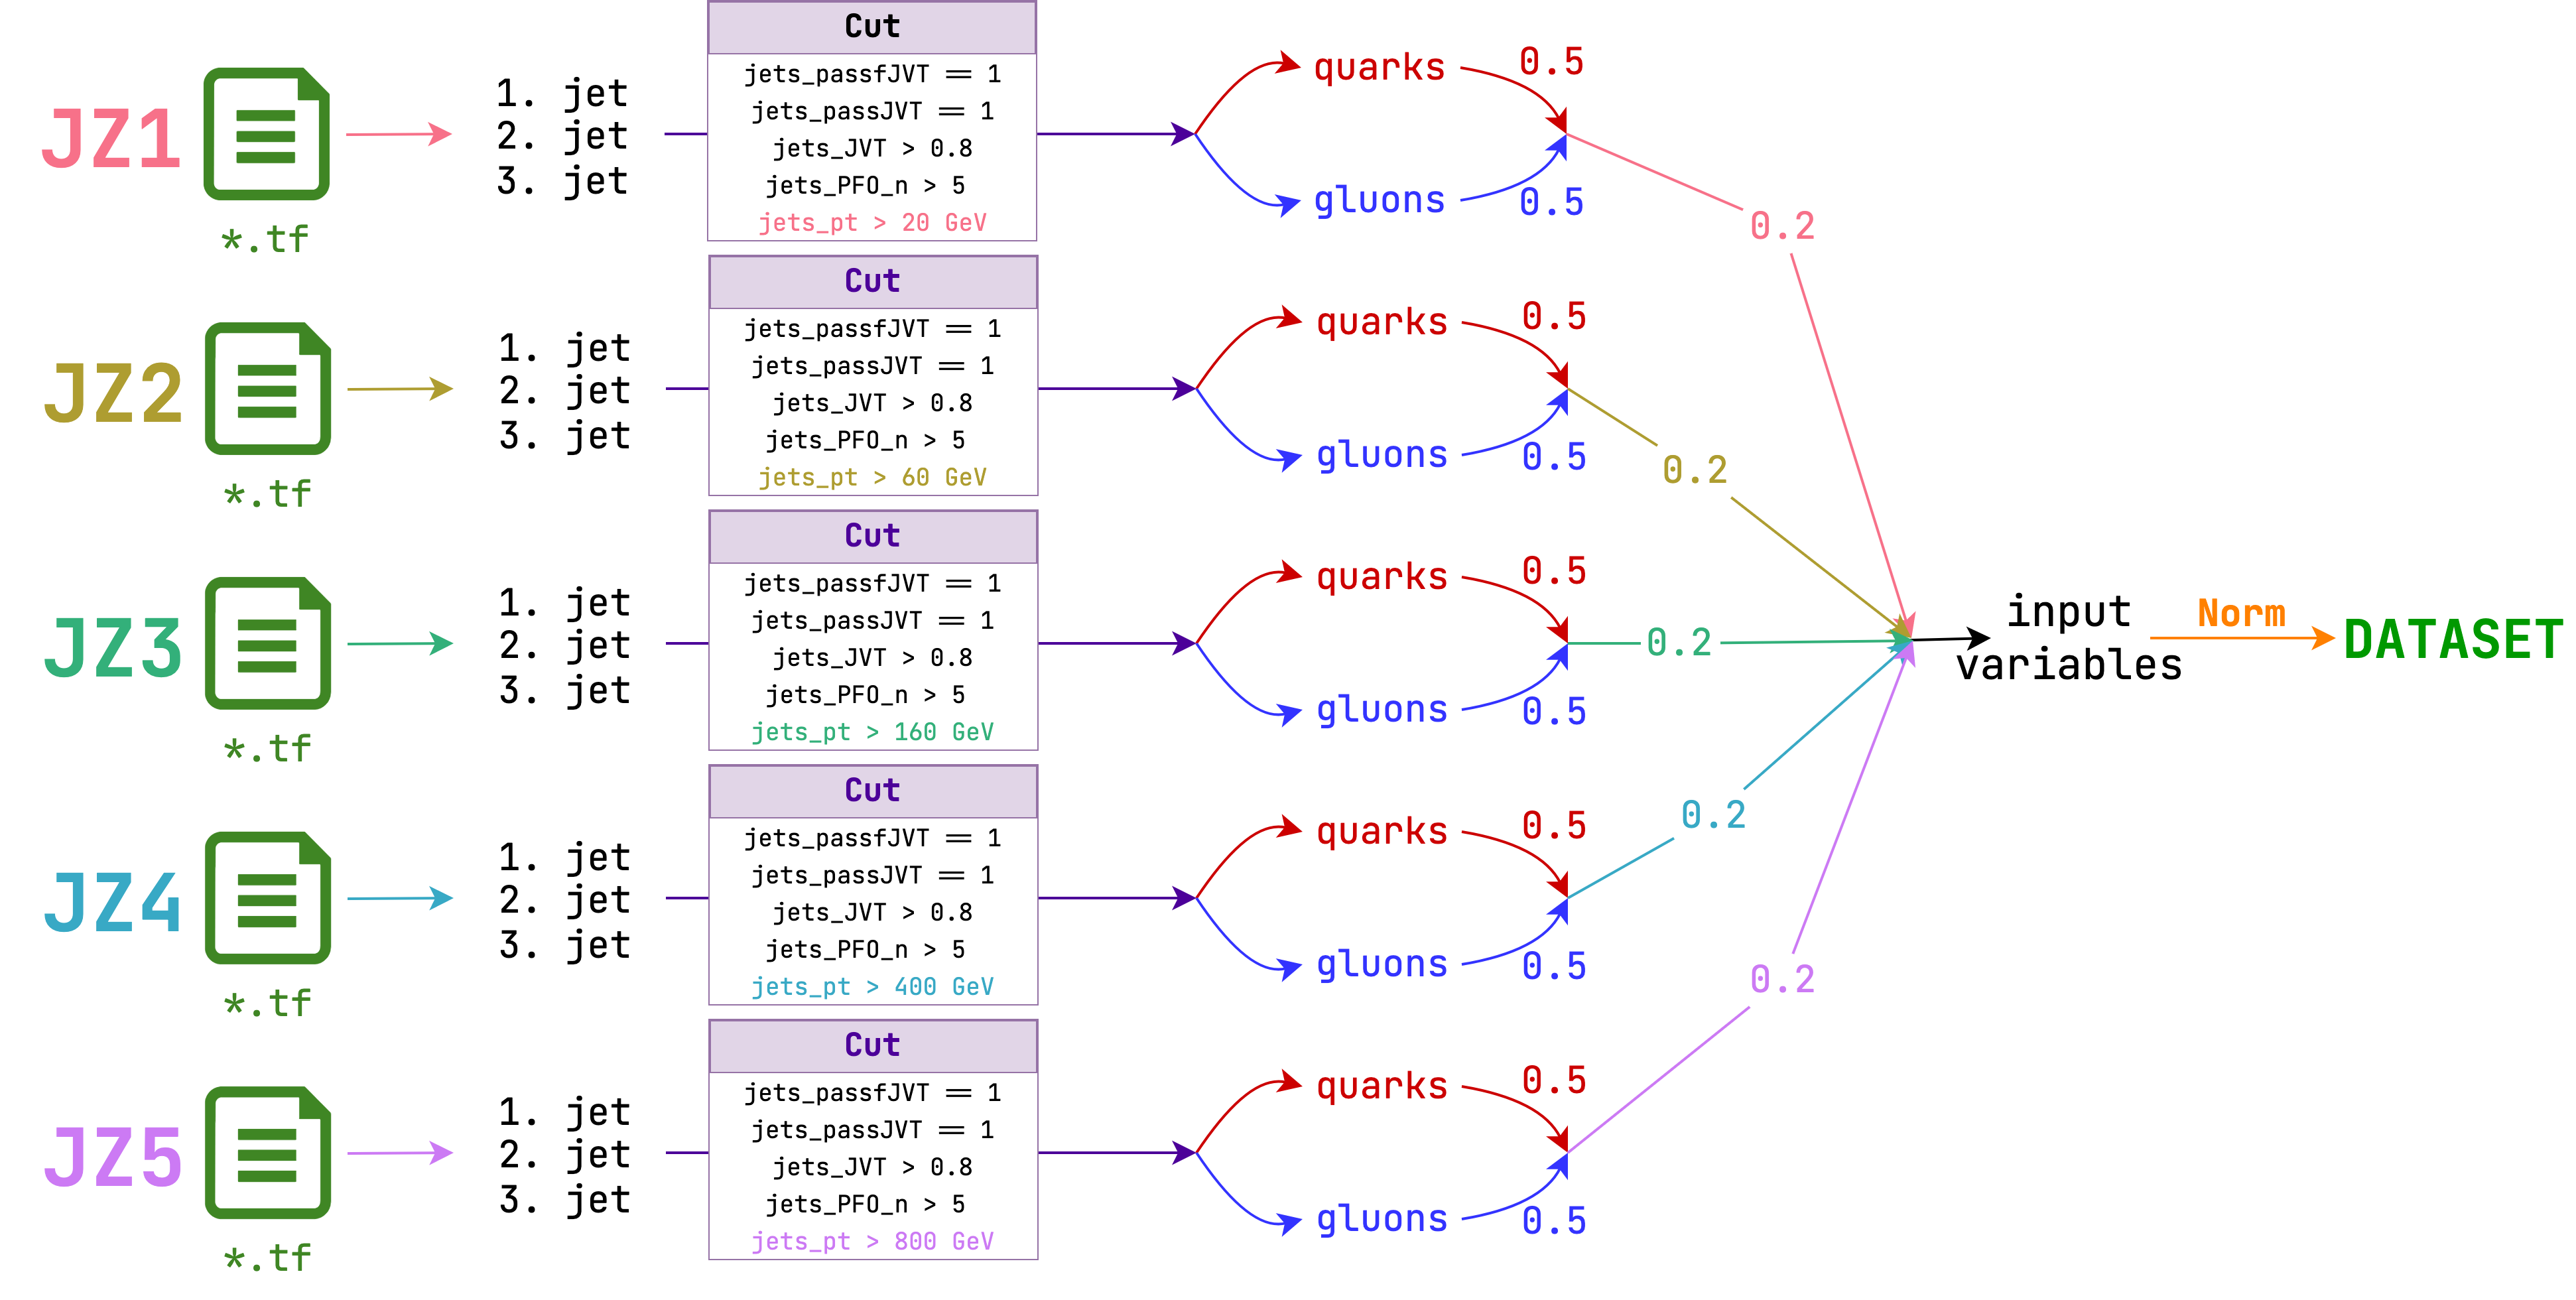
\includegraphics[width=1.\textwidth]{src/diagrams/data_prep_on.png}
    \caption{The online preprocessing of the data.}
    \label{fig:data_prep_on}
\end{figure}
The online preprocessing utilizing the \texttt{tf.data.Dataset} API, allowing pipeline construction of the dataset, which is done with the training process. 
Our preprocessing pipeline consists of the following steps:
\begin{enumerate}
    \item Load each JZ slice separately.
    \item Filter data with the following cuts:
    \begin{itemize}
        \item \texttt{jets\_passFJVT} $== 1$,
        \item \texttt{jets\_passJVT} $== 1$,
        \item \texttt{jets\_Jvt} $> 0.8$,
        \item \texttt{jets\_PFO\_n} $> 5$,
        \item \texttt{jets\_pt} $>$ \textit{(based on JZ slice, see \cref{sec:jet_pt_cuts})},
    \end{itemize}
    \item For each JZ slice, resample the quark and gluon datasets, each with probability 0.5,  
    \item Combine JZ slices, each with the same probability (0.2 for each JZ slice when JZ slices 1-5 are used),
    \item Construct desired input variables,
    \item Normalize the input variables,
\end{enumerate}

In step 2, we apply cut on the jet variables estimating the amount of pileup.
We do not want to train on pileup jets, so we filter them out as much as possible using the abovementioned cuts.
The PFO-based taggers need some minimum number of \PFOs to work correctly, so we filter out jets with less than 5 \PFOs.

We apply a cut on the jet $\pT$ based on the JZ slice to make the spectrum for quarks and gluons more similar.
This is extensively discussed in \cref{sec:jet_pt_cuts}.

Resampling the quark and gluon datasets is done to make the dataset balanced.
We can obtain the same result by reweighting each jet, but we have no prior knowledge of the weights.
The method \texttt{tf.data. dataset.rejection\_resample}\footnote{\url{https://www.tensorflow.org/api_docs/python/tf/data/Dataset\#rejection\_resample}} allows resampling on the go by computing the ratio dynamically as the data is processed.

Combining JZ slices with equal probability ensures the model works on the full spectrum of jets. 
This is a non-trivial step, as in actual physical data, the jet $\pT$ spectrum is highly dominated by low $\pT$ jets, while the high $\pT$ jets are rare. 
However, some applications are specifically interested in the high $\pT$ jets, so we want to ensure the model can also handle them.

The construction of variables and their normalization is explained \cref{sec:input_variables}.
The whole process is illustrated in \cref{fig:data_prep_on}.


\subsection{JZ Cuts}
\label{sec:jet_pt_cuts}

\begin{figure}[htb]
    \centering
    \begin{subfigure}[t]{0.49\textwidth}
        \centering
        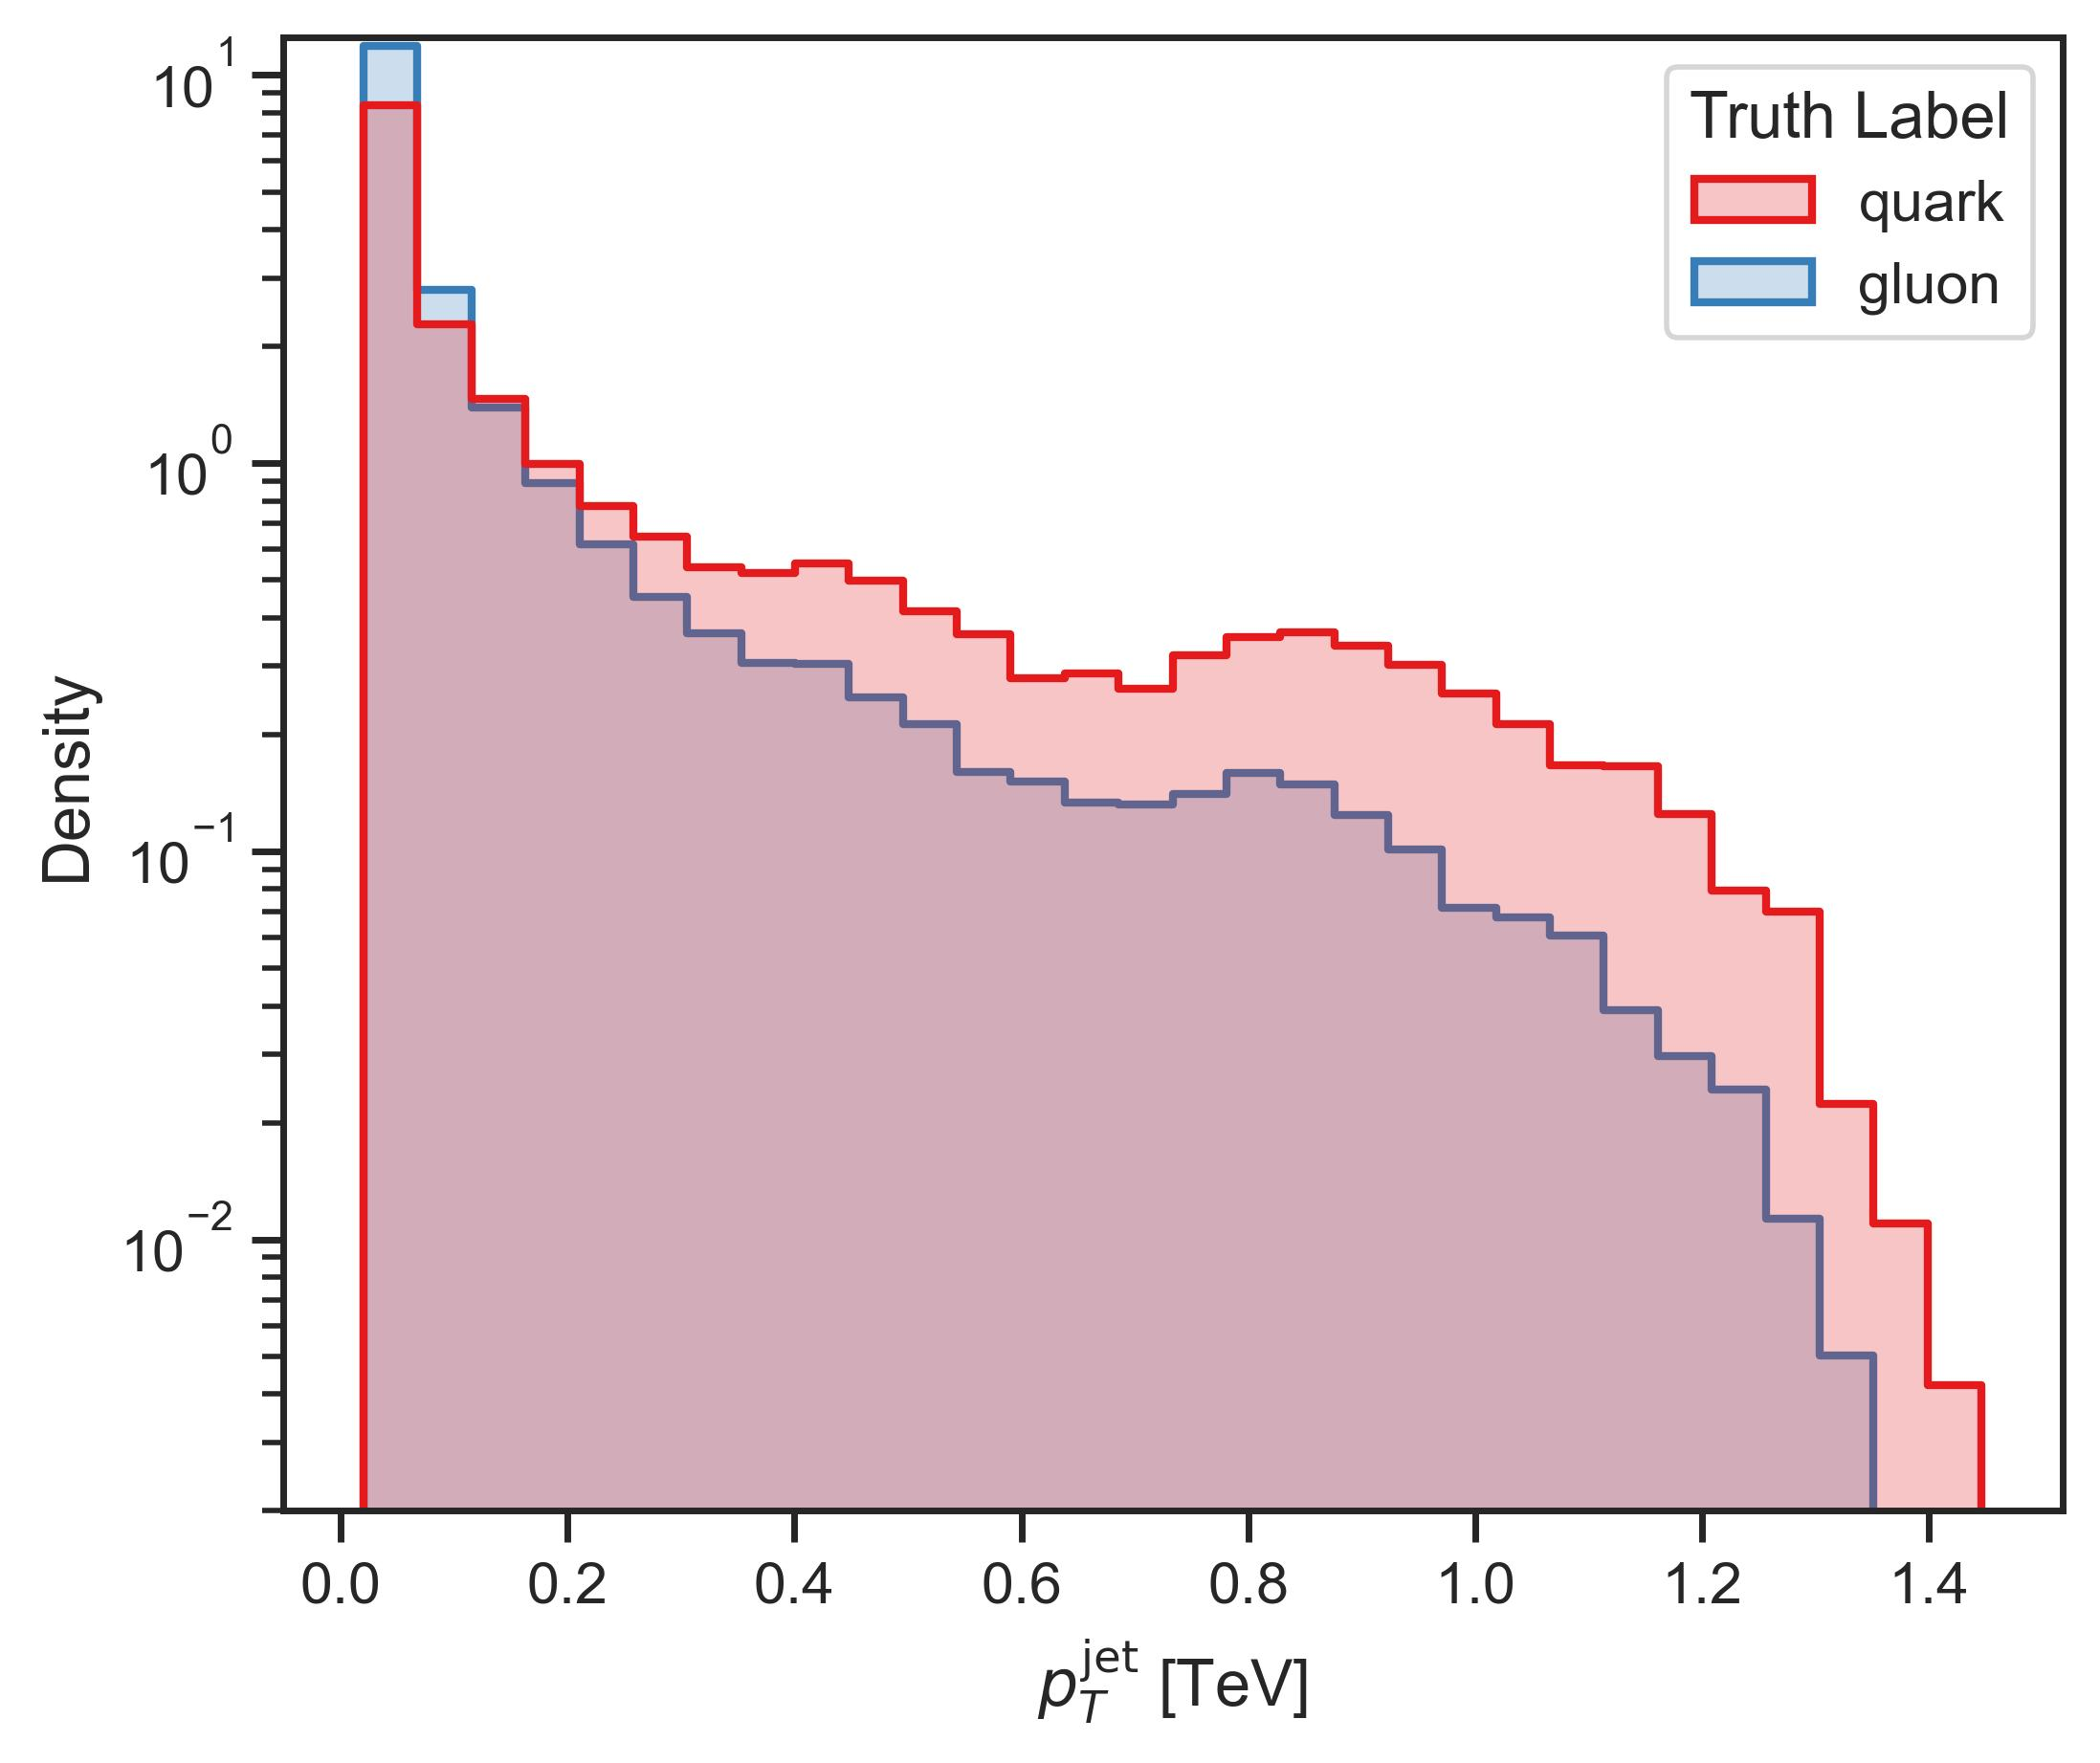
\includegraphics[width=\linewidth]{src/plots/pt_jet_label.jpg}
        \caption{colored by their Truth Label}
        \label{fig:jz_all_label}
    \end{subfigure}
    \begin{subfigure}[t]{0.49\textwidth}
        \centering
        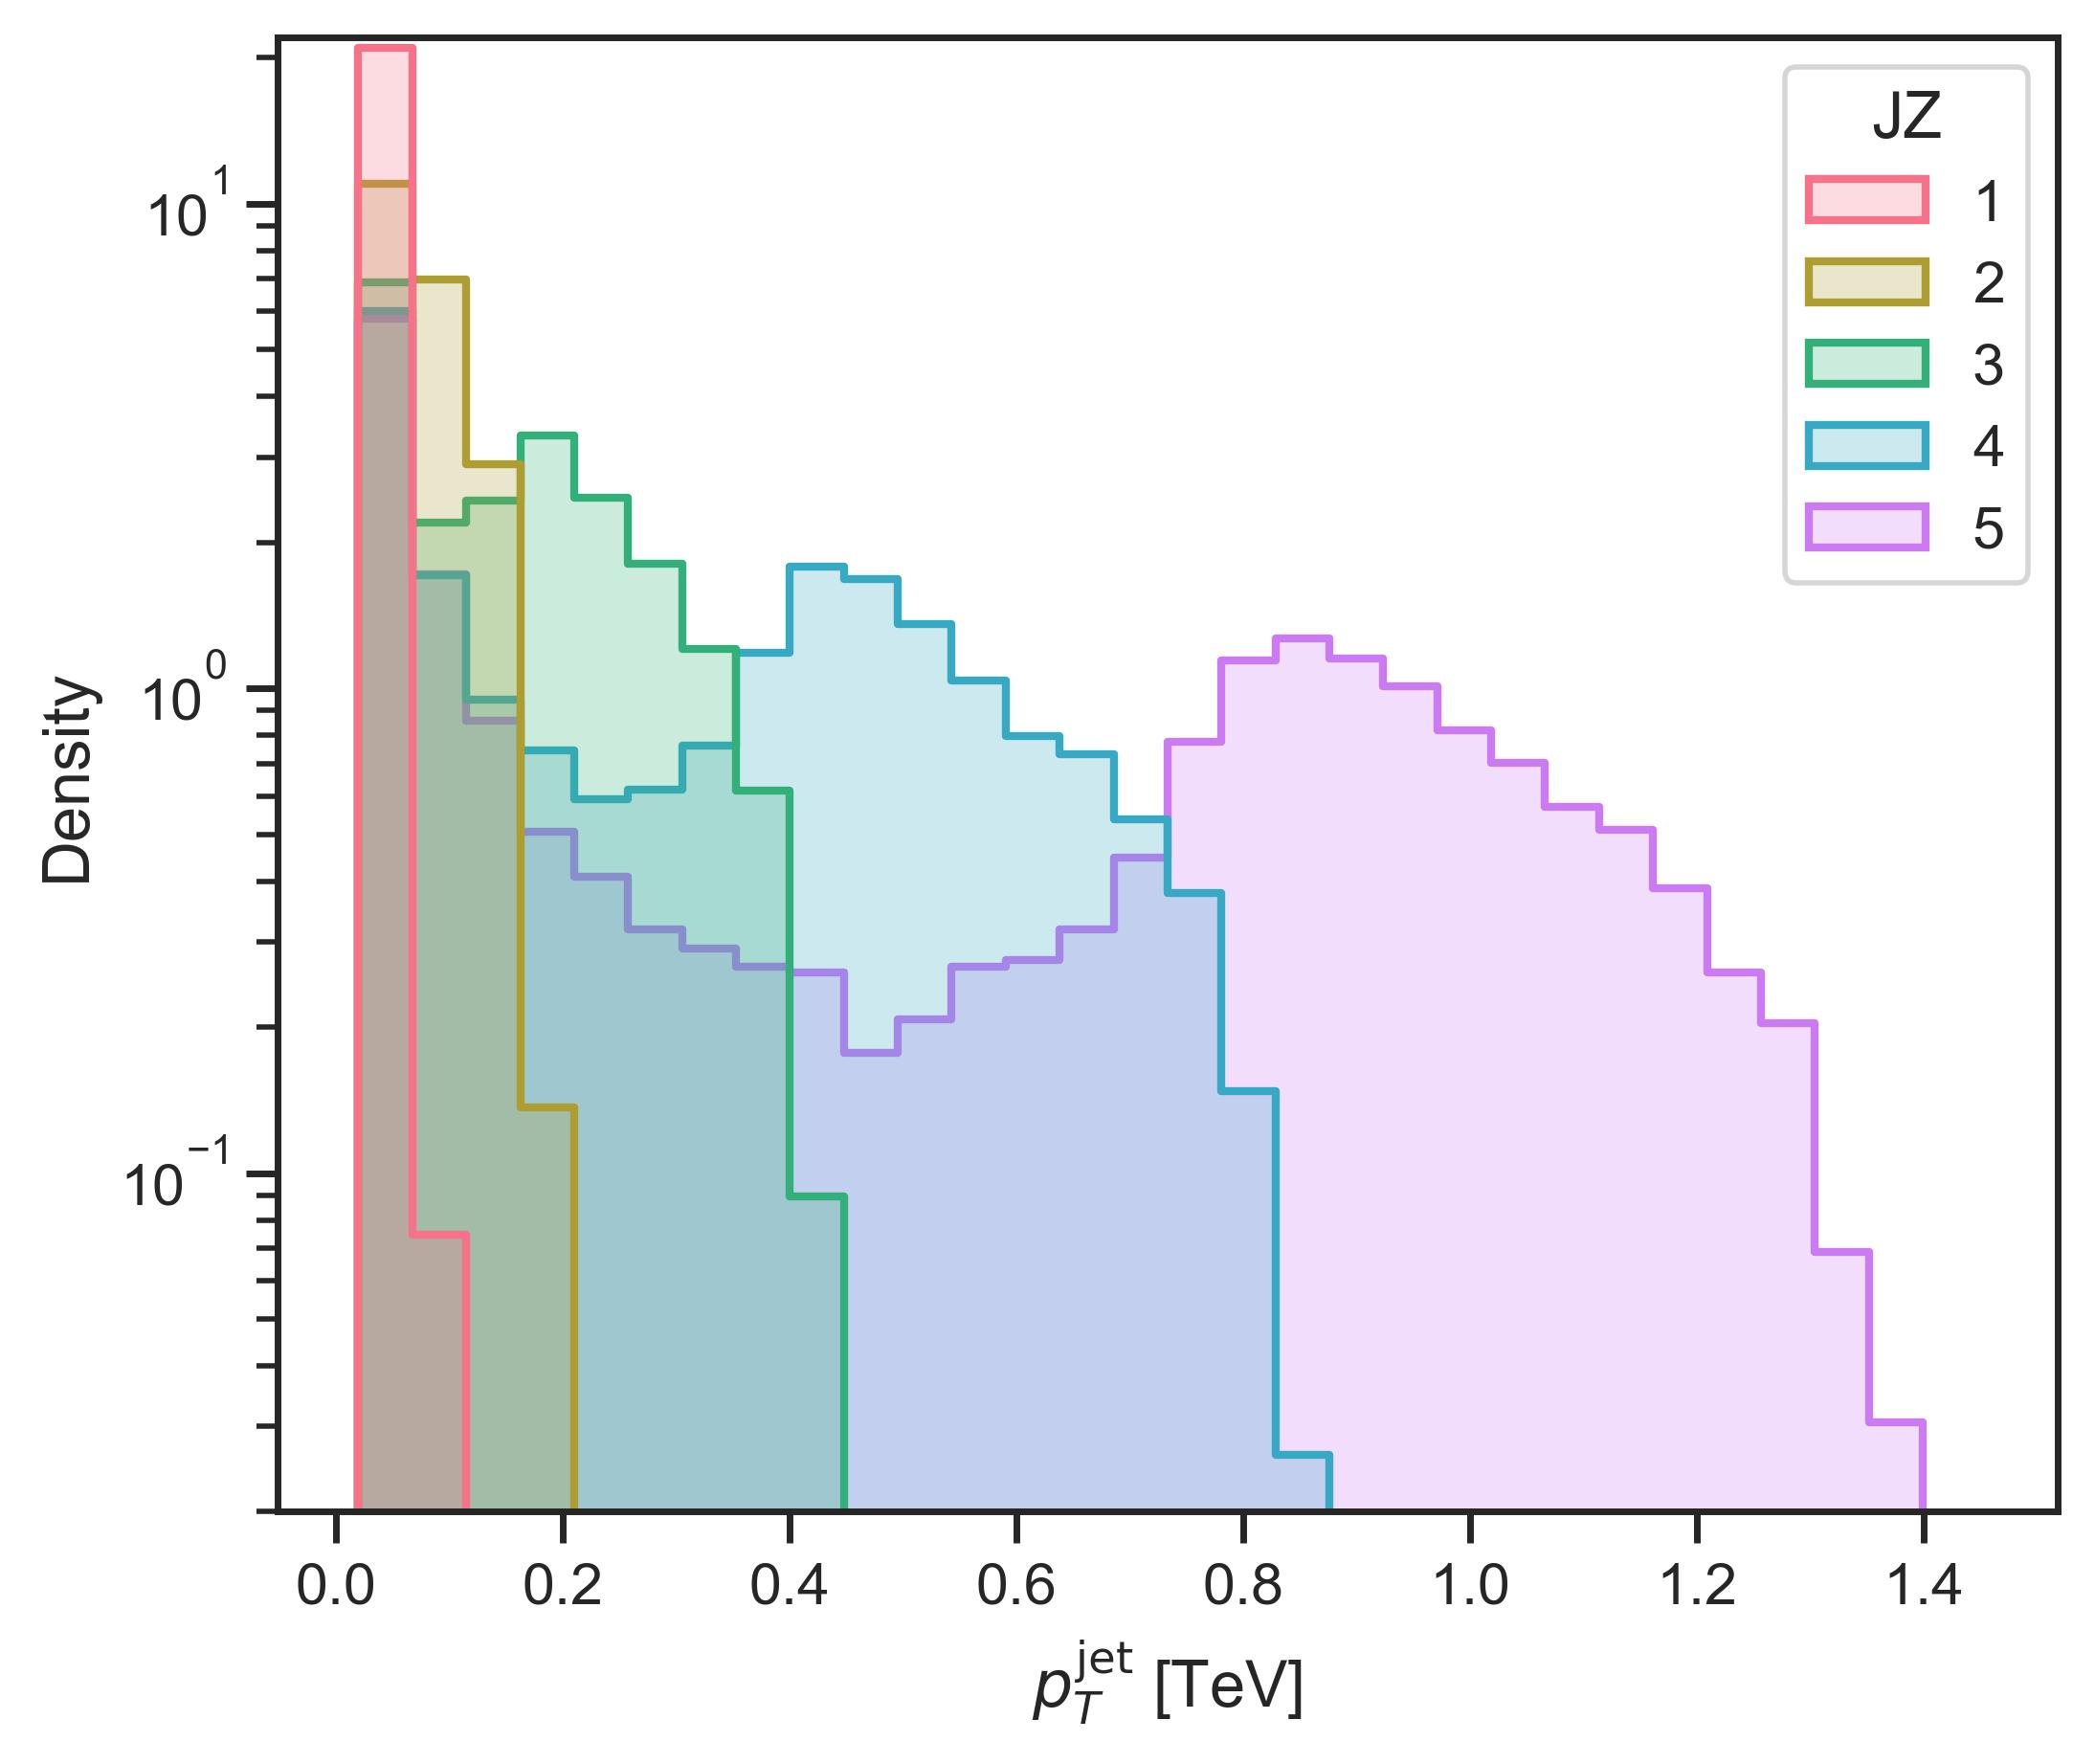
\includegraphics[width=\linewidth]{src/plots/pt_jet_jz.jpg}
        \caption{colored by their JZ slice}
        \label{fig:jz_all_jz}
    \end{subfigure}
    \caption{Normalized $\pT$ distributions of jets \emph{before} the JZ \emph{cuts} are applied.}
    \label{fig:jz_all}
\end{figure}
As stated in \cref{sec:event_production}, data is split into JZ slices, each having a different $\pT$ distribution.
The distribution of the jet $\pT$ is shown in \cref{fig:jz_all}.
The number of quarks and gluons is the same.

\begin{figure}[!htb]
    \centering
    \begin{subfigure}[t]{0.49\textwidth}
        \centering
        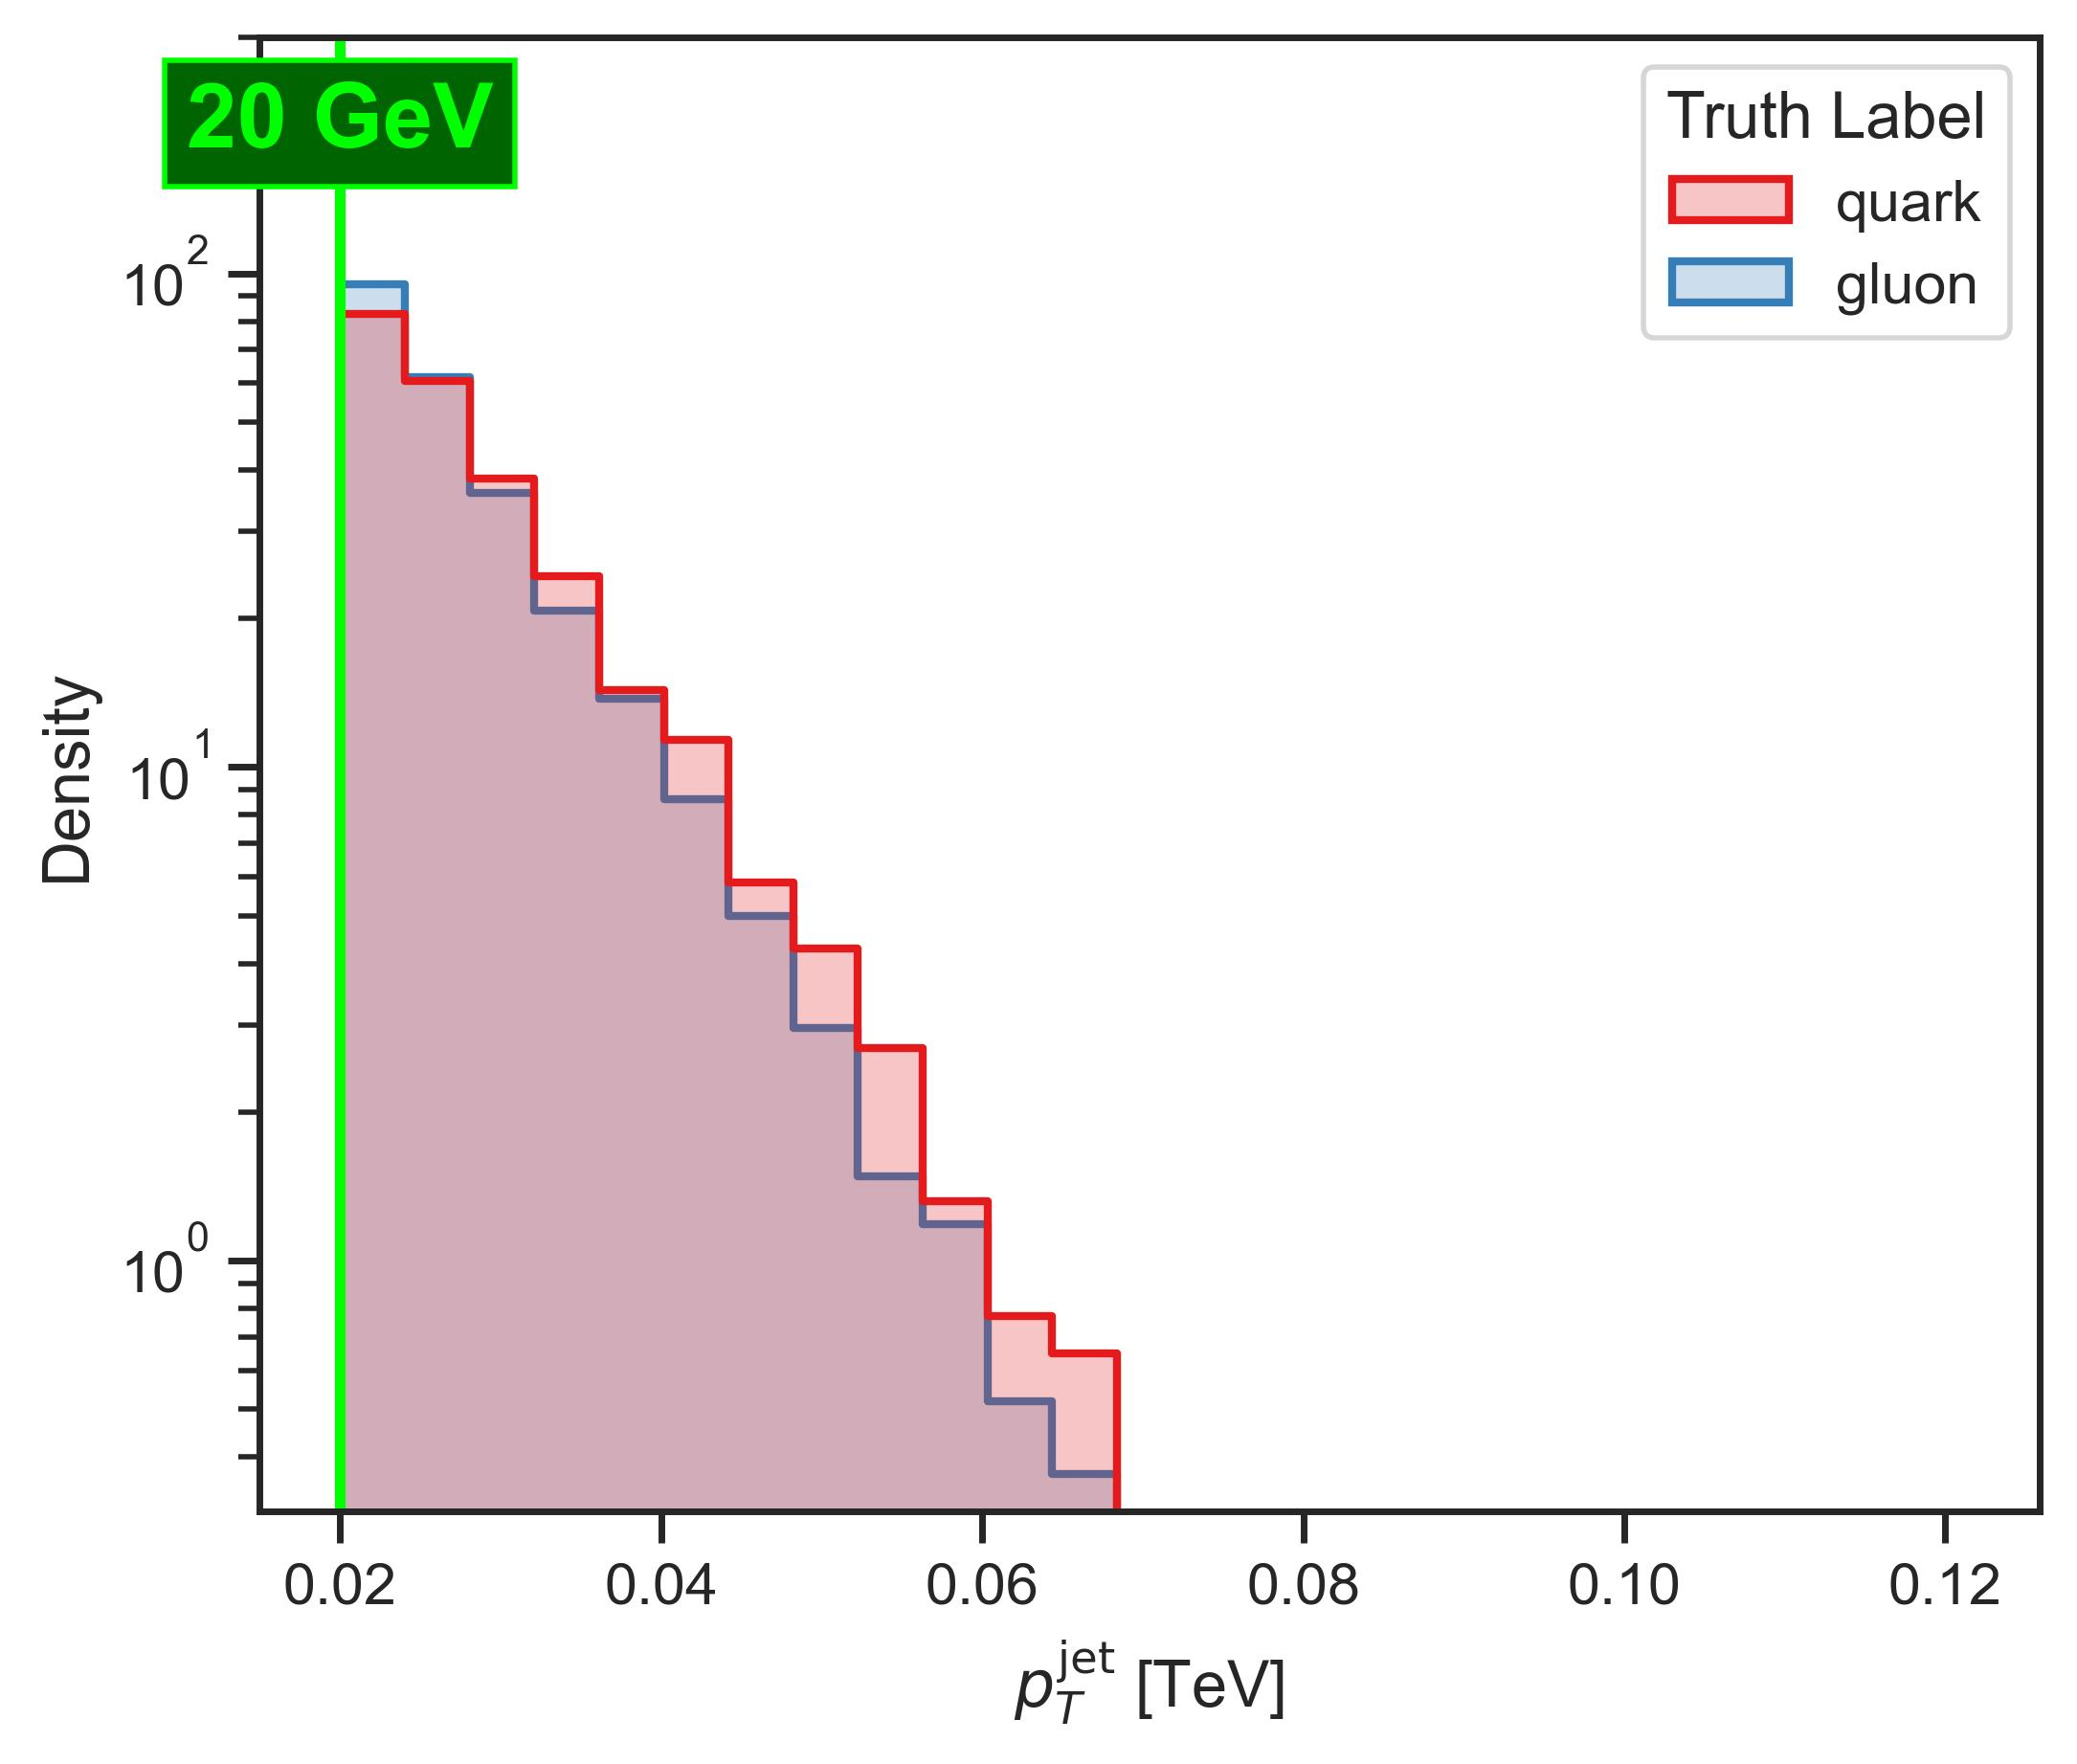
\includegraphics[width=\linewidth]{src/plots/pt_jet_label_1.jpg}
        \caption{JZ slice 1, 20 GeV cut}
        \label{fig:jz_separete_1}
    \end{subfigure}
    \begin{subfigure}[t]{0.49\textwidth}
        \centering
        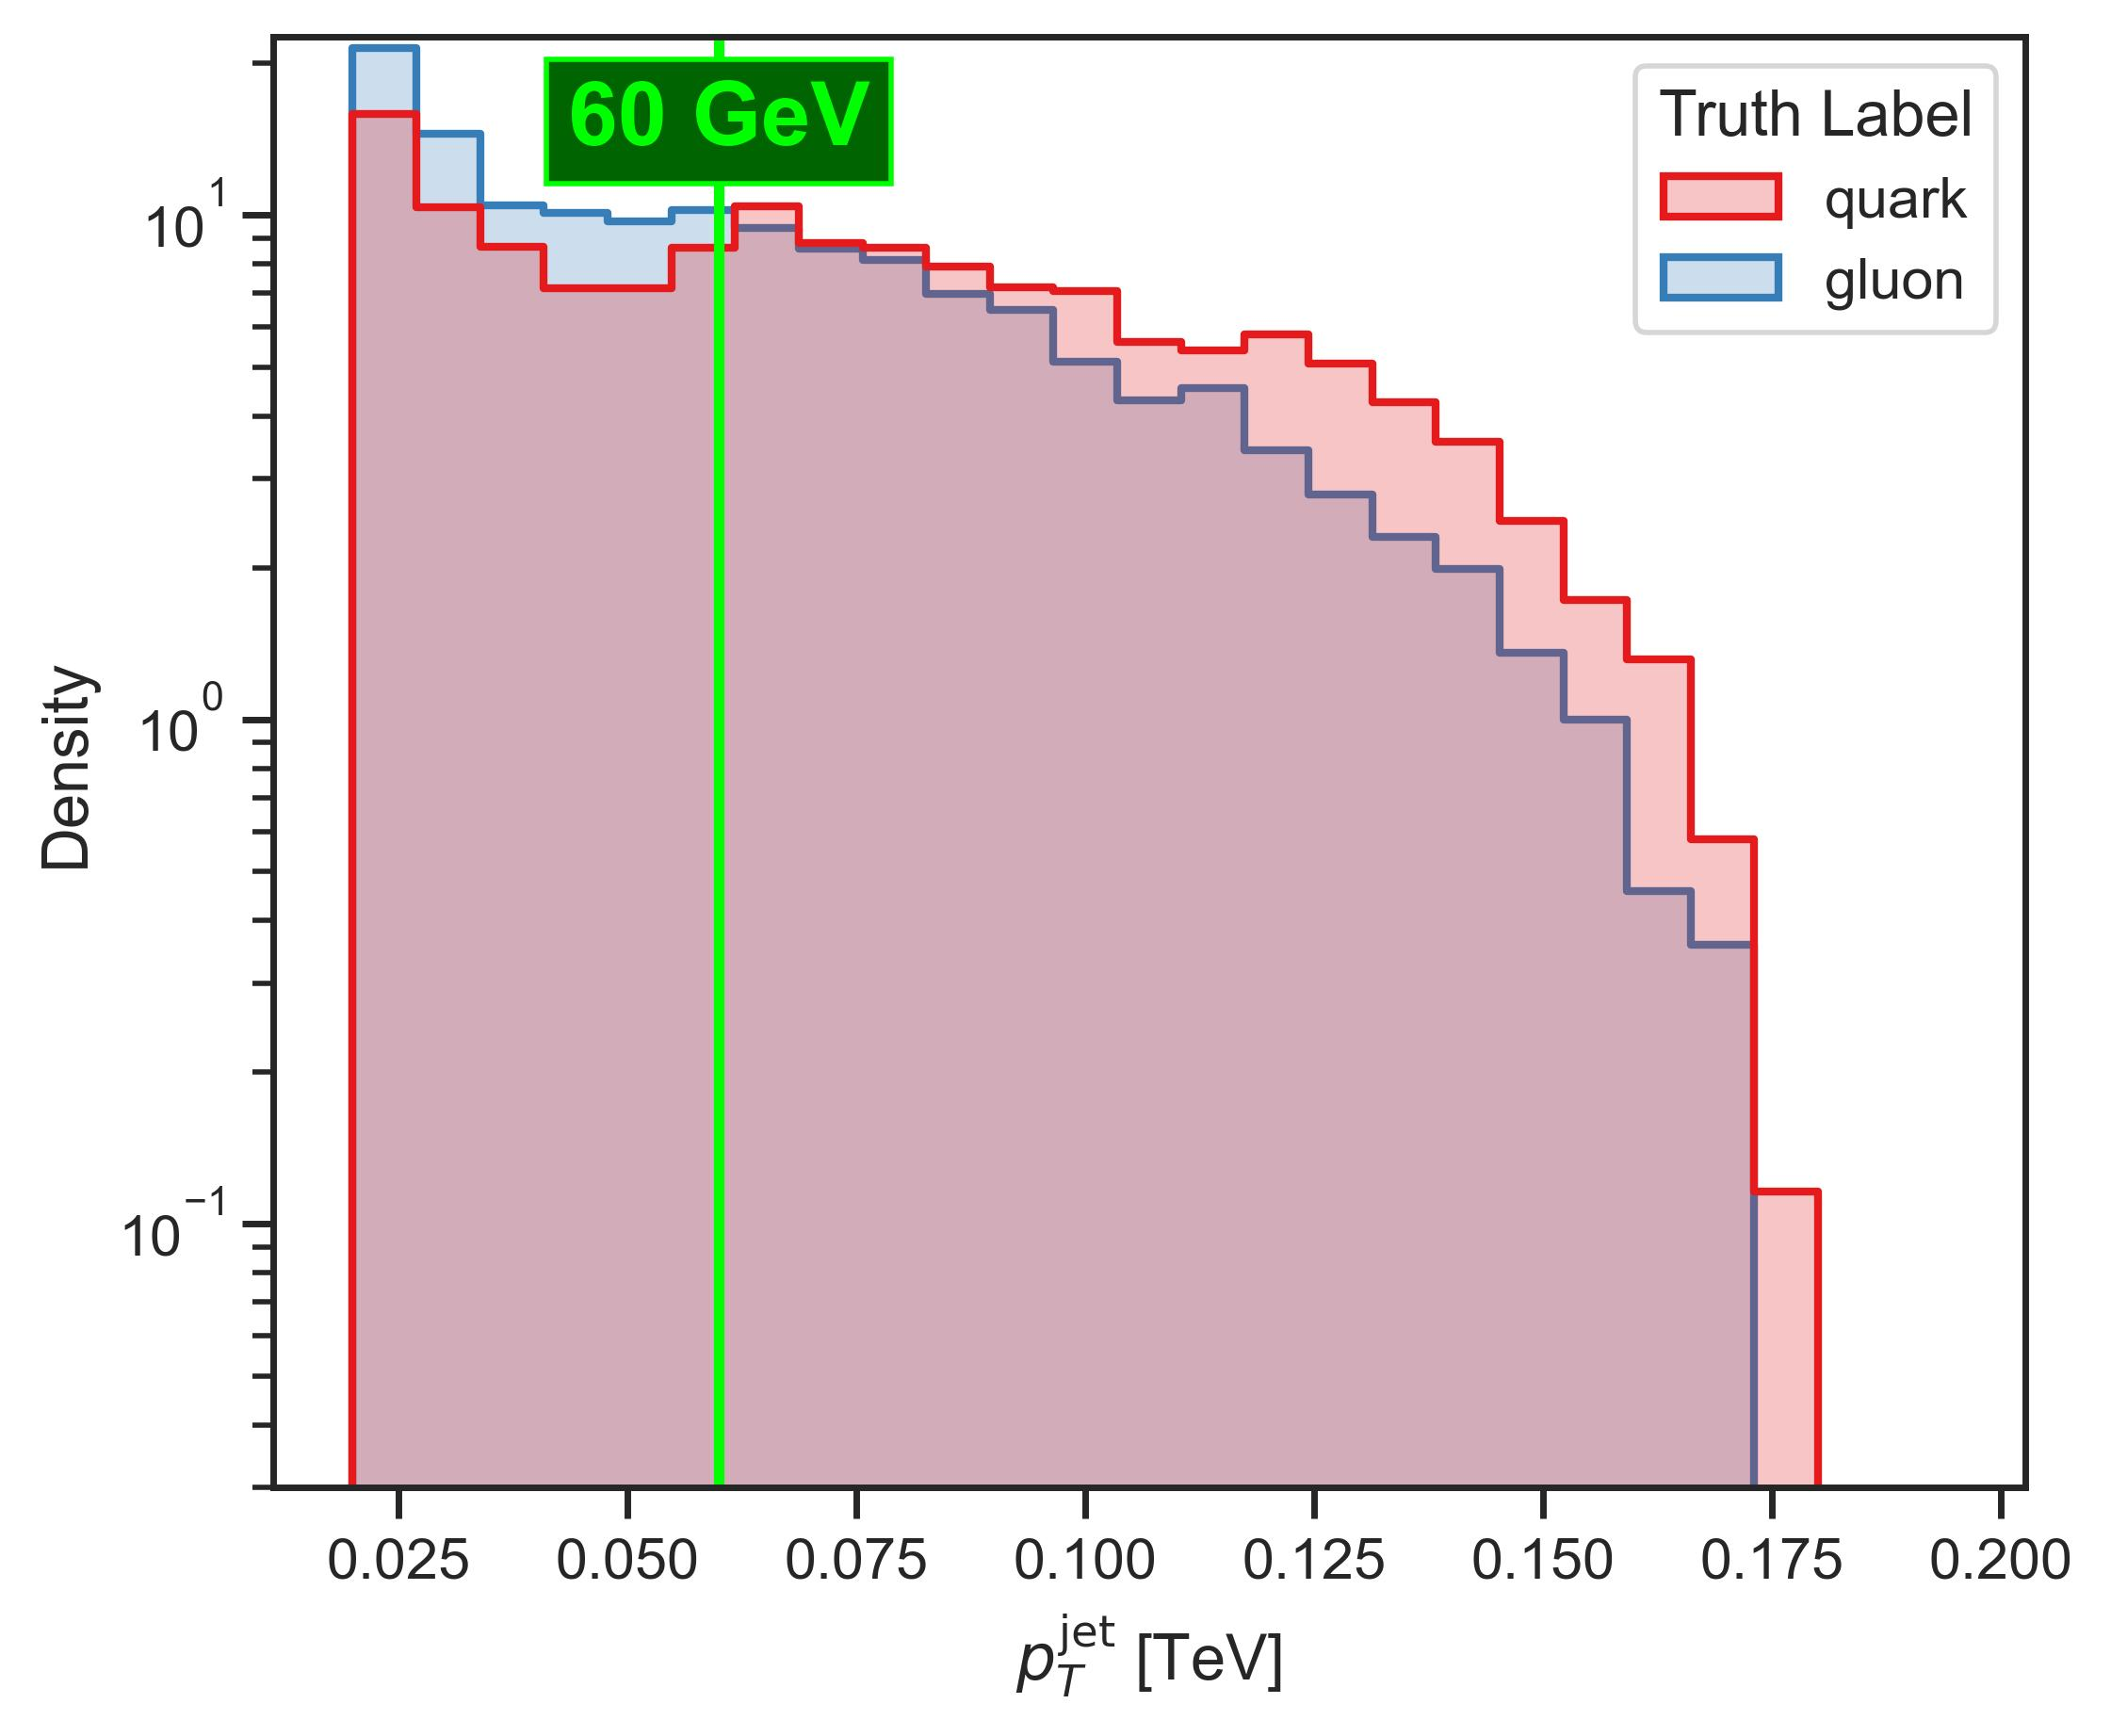
\includegraphics[width=\linewidth]{src/plots/pt_jet_label_2.jpg}
        \caption{JZ slice 2, 60 GeV cut}
        \label{fig:jz_separete_2}
    \end{subfigure}
    \begin{subfigure}[t]{0.49\textwidth}
        \centering
        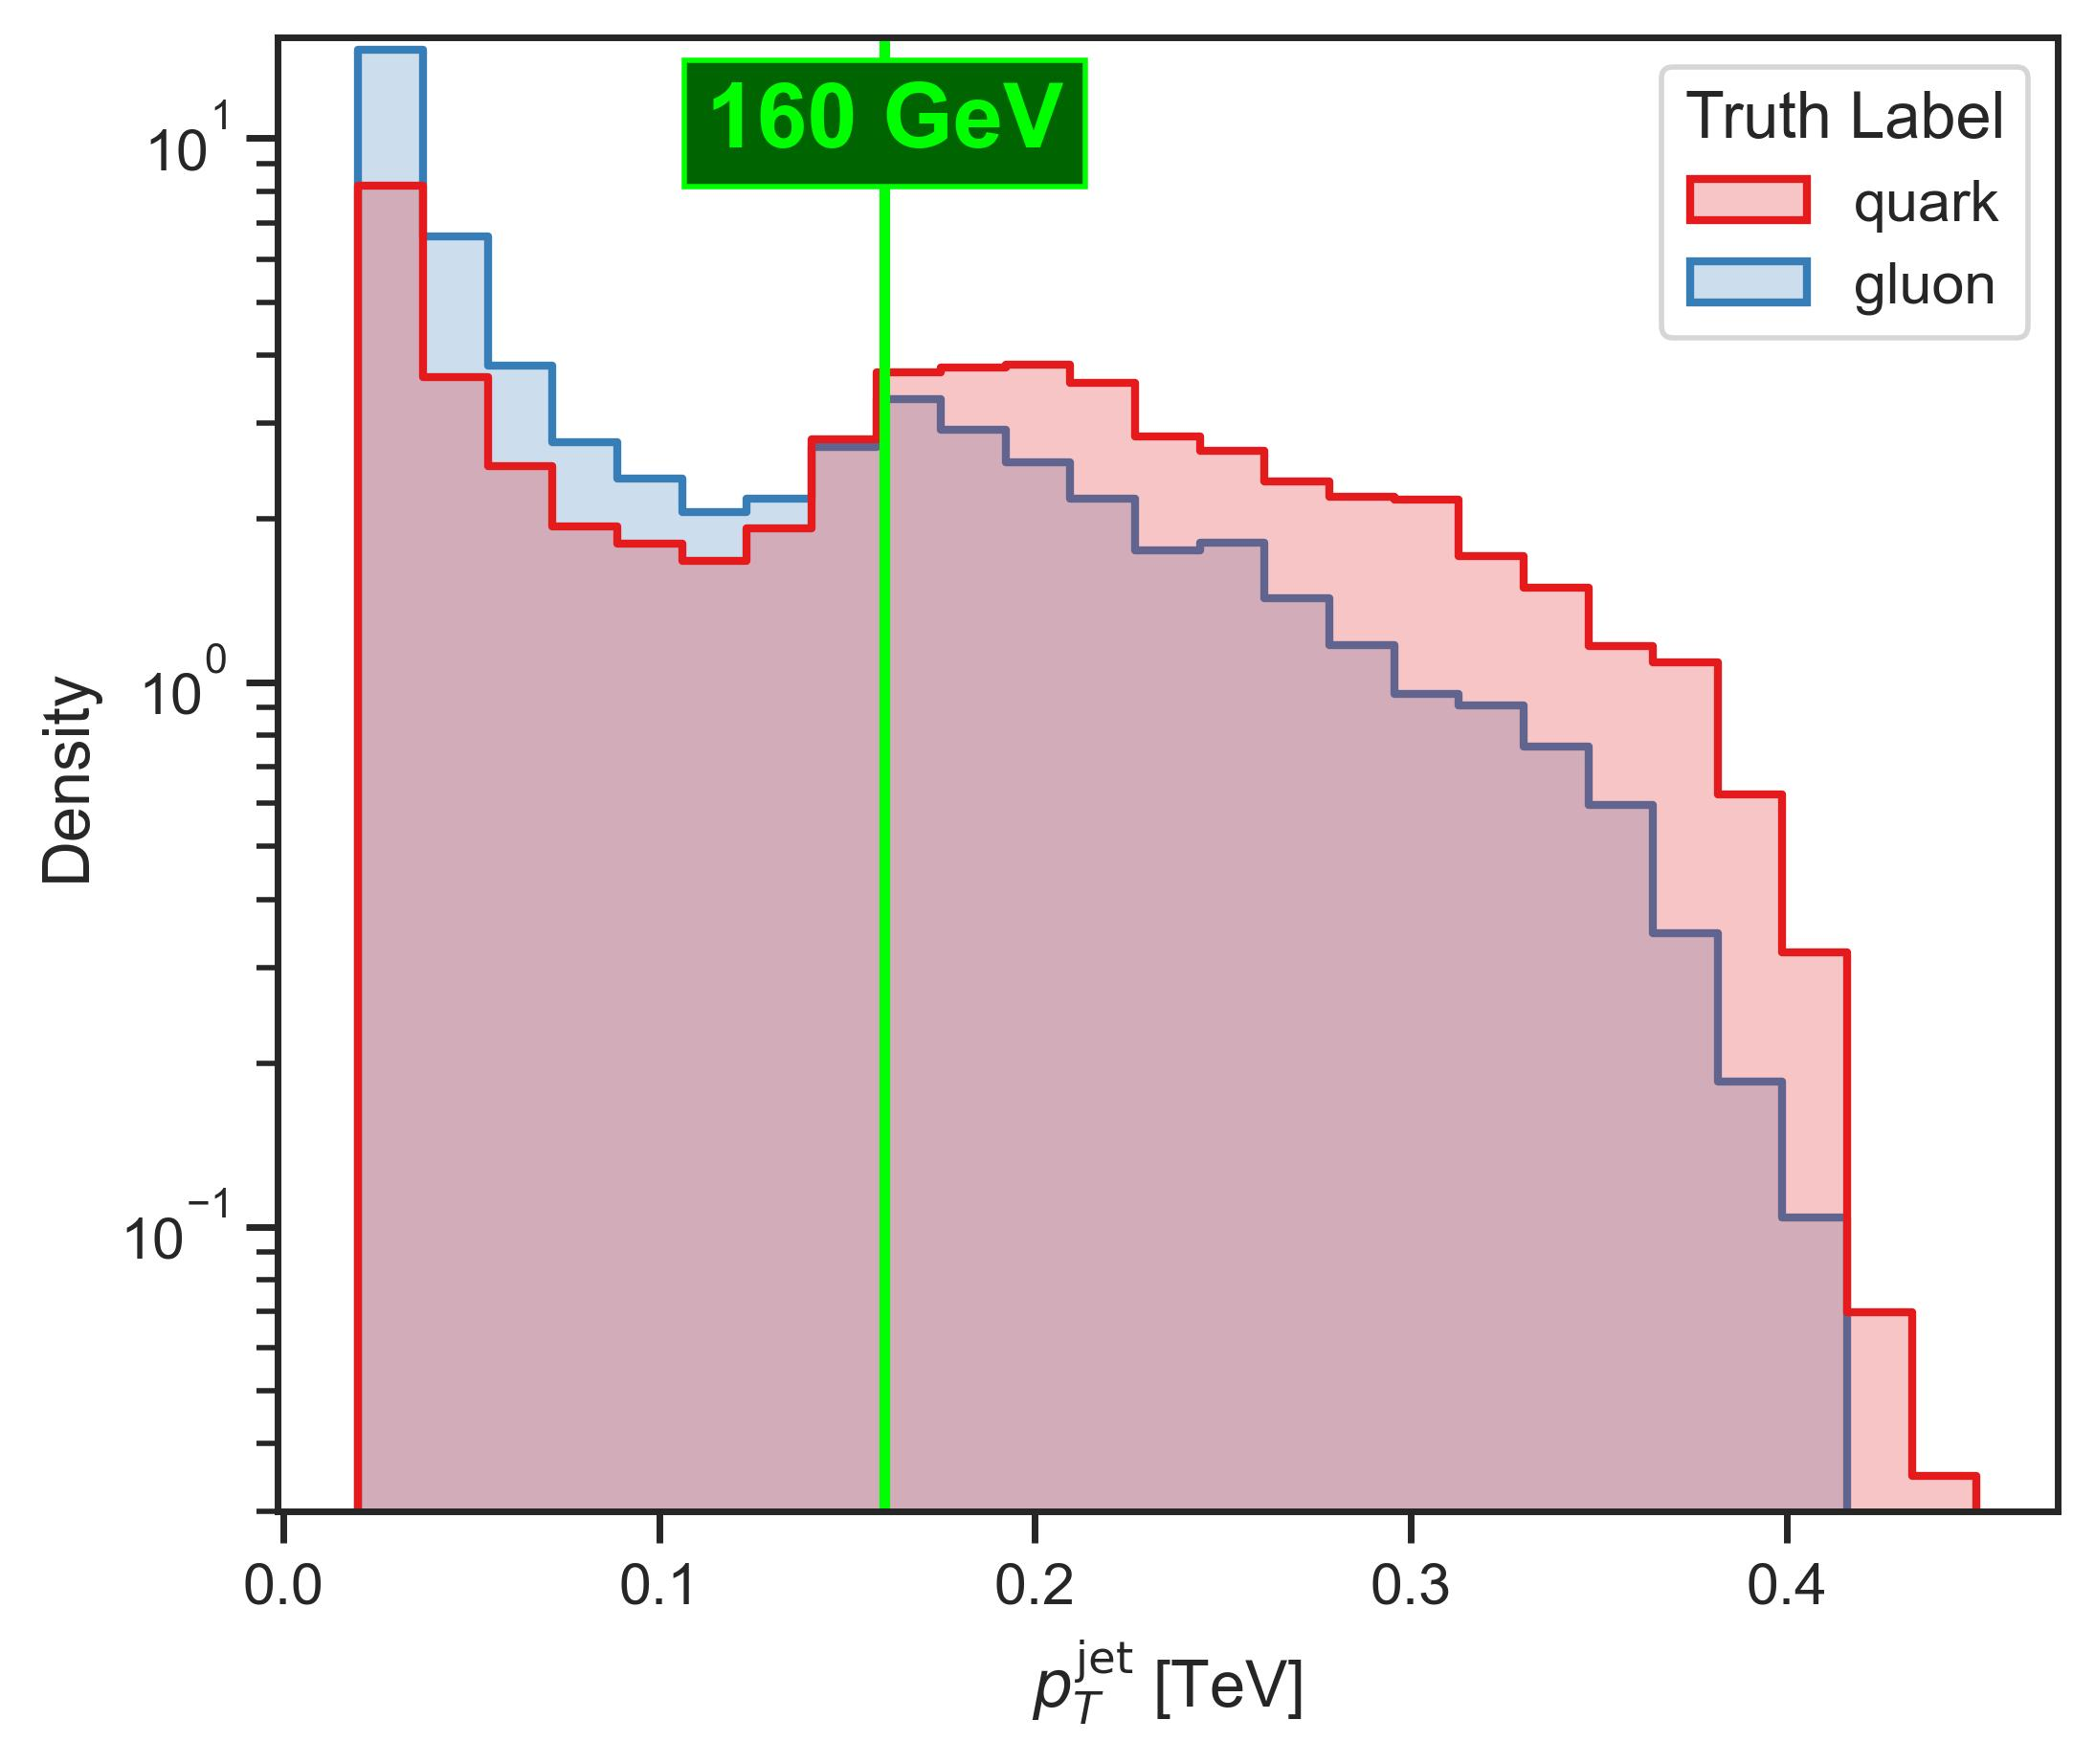
\includegraphics[width=\linewidth]{src/plots/pt_jet_label_3.jpg}
        \caption{JZ slice 3, 160 GeV cut}
        \label{fig:jz_separete_3}
    \end{subfigure}
    \begin{subfigure}[t]{0.49\textwidth}
        \centering
        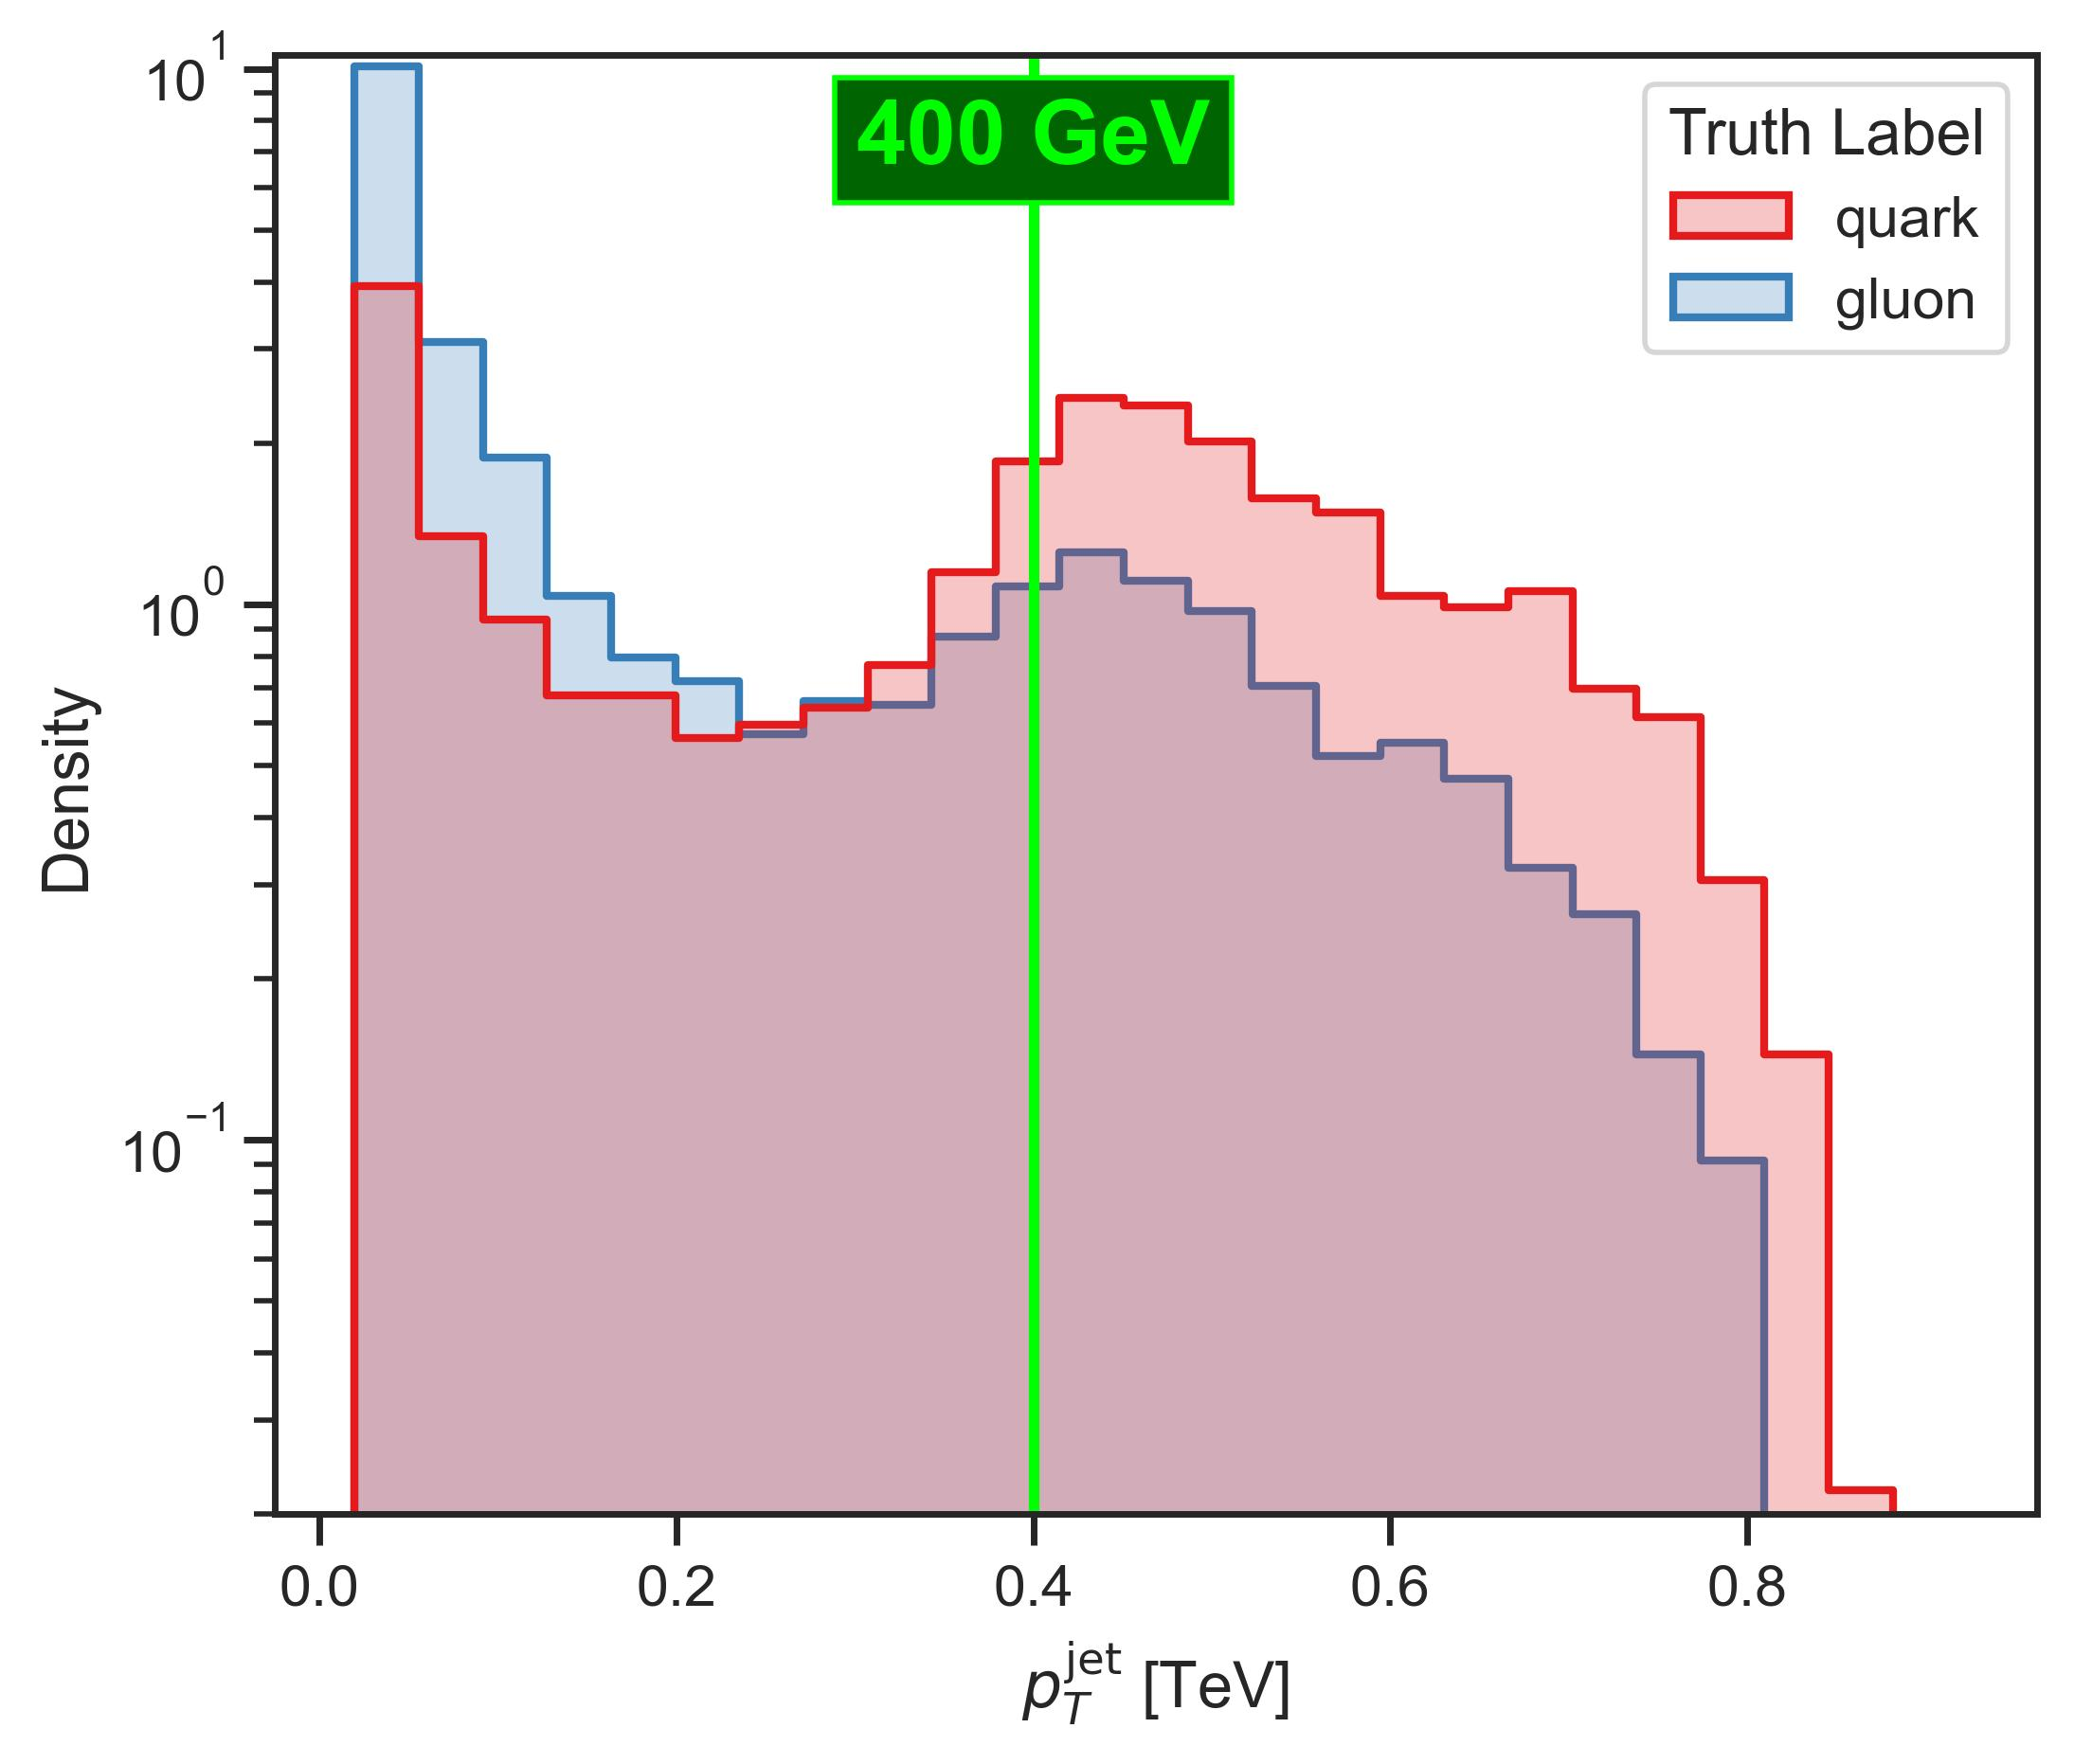
\includegraphics[width=\linewidth]{src/plots/pt_jet_label_4.jpg}
        \caption{JZ slice 4, 400 GeV cut}
        \label{fig:jz_separete_4}
    \end{subfigure}
    \begin{subfigure}[t]{0.49\textwidth}
        \centering
        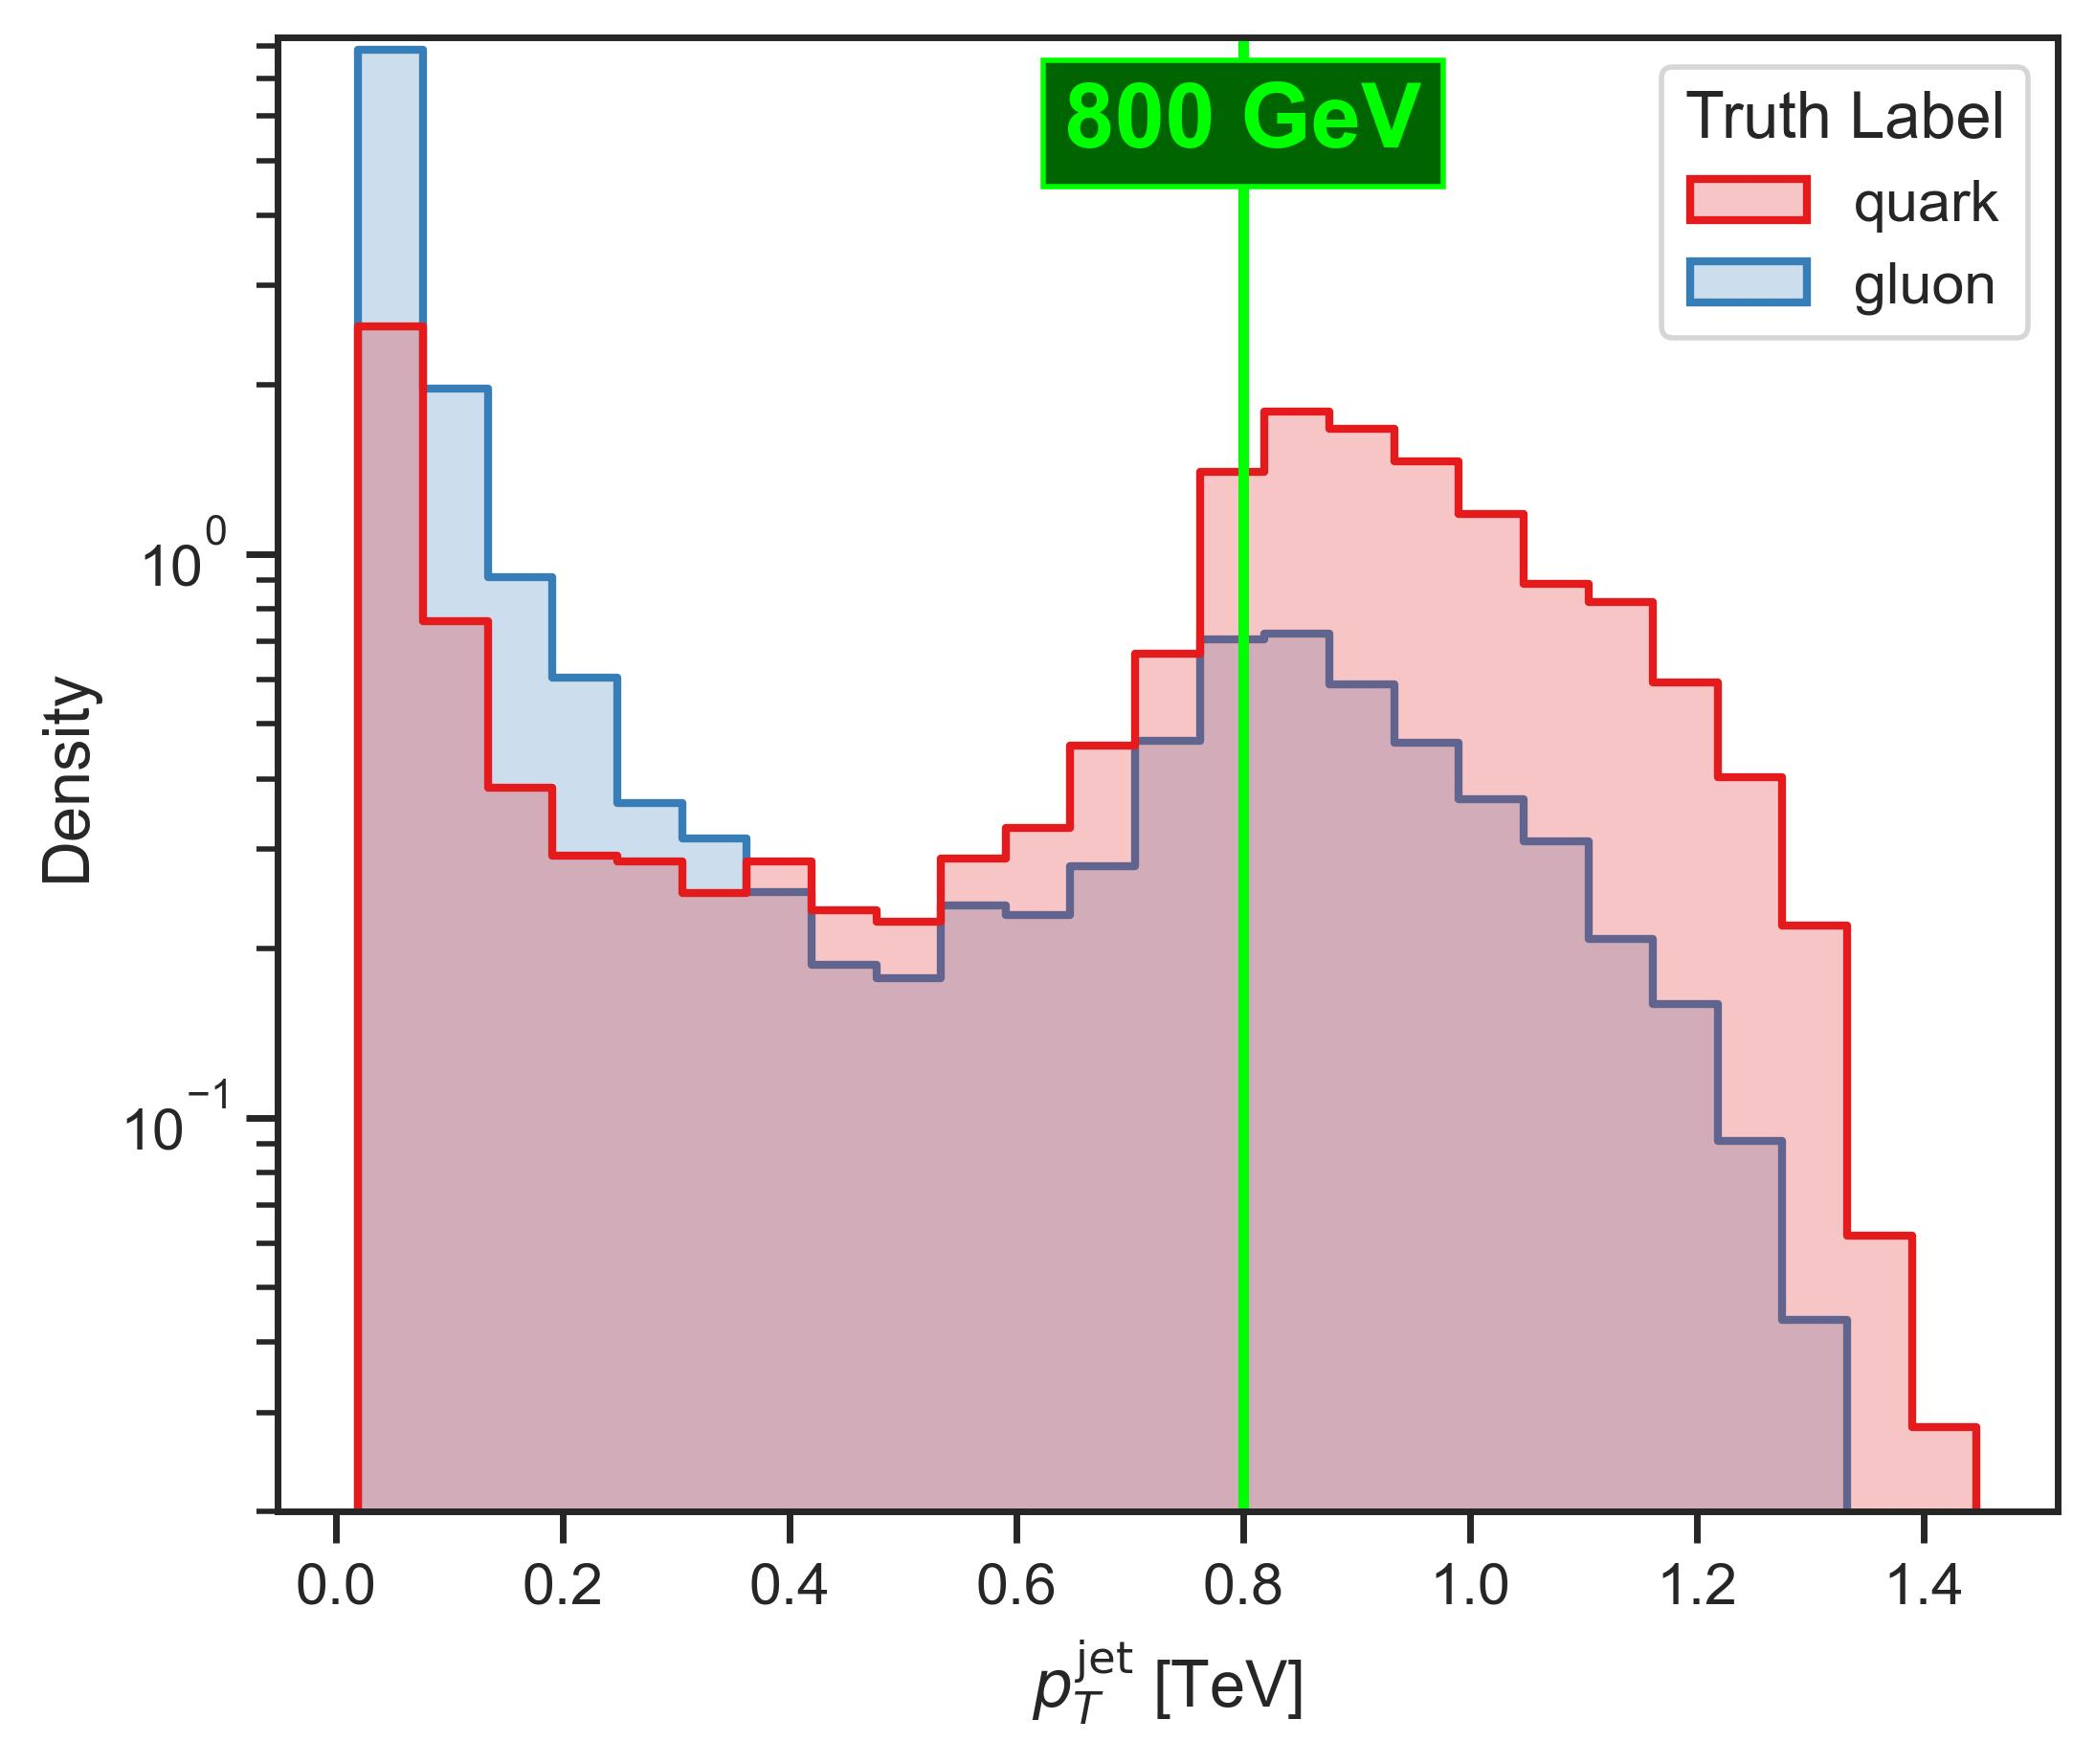
\includegraphics[width=\linewidth]{src/plots/pt_jet_label_5.jpg}
        \caption{JZ slice 5, 800 GeV cut}
        \label{fig:jz_separete_5}
    \end{subfigure}
    \caption{Normalized $\pT$ distributions of jets after the JZ cuts are applied.}
    \label{fig:jz_separete}
\end{figure}

From \cref{fig:jz_all_label}, we can see that the $\pT$ distribution of the jets is different for each Truth Label.
Gluons dominate the low $\pT$ region \footnote{This might not be obvious, but pay attention to the log scale of the y-axis.}, while quarks dominate the high $\pT$ region.
All JZ slices contribute to these low $\pT$ regions, mainly with soft gluon jets.
This can be seen from \cref{fig:jz_separete}, where all JZ slices are shown separately.
\begin{figure}[htb]
    \centering
    \begin{subfigure}[t]{0.49\textwidth}
        \centering
        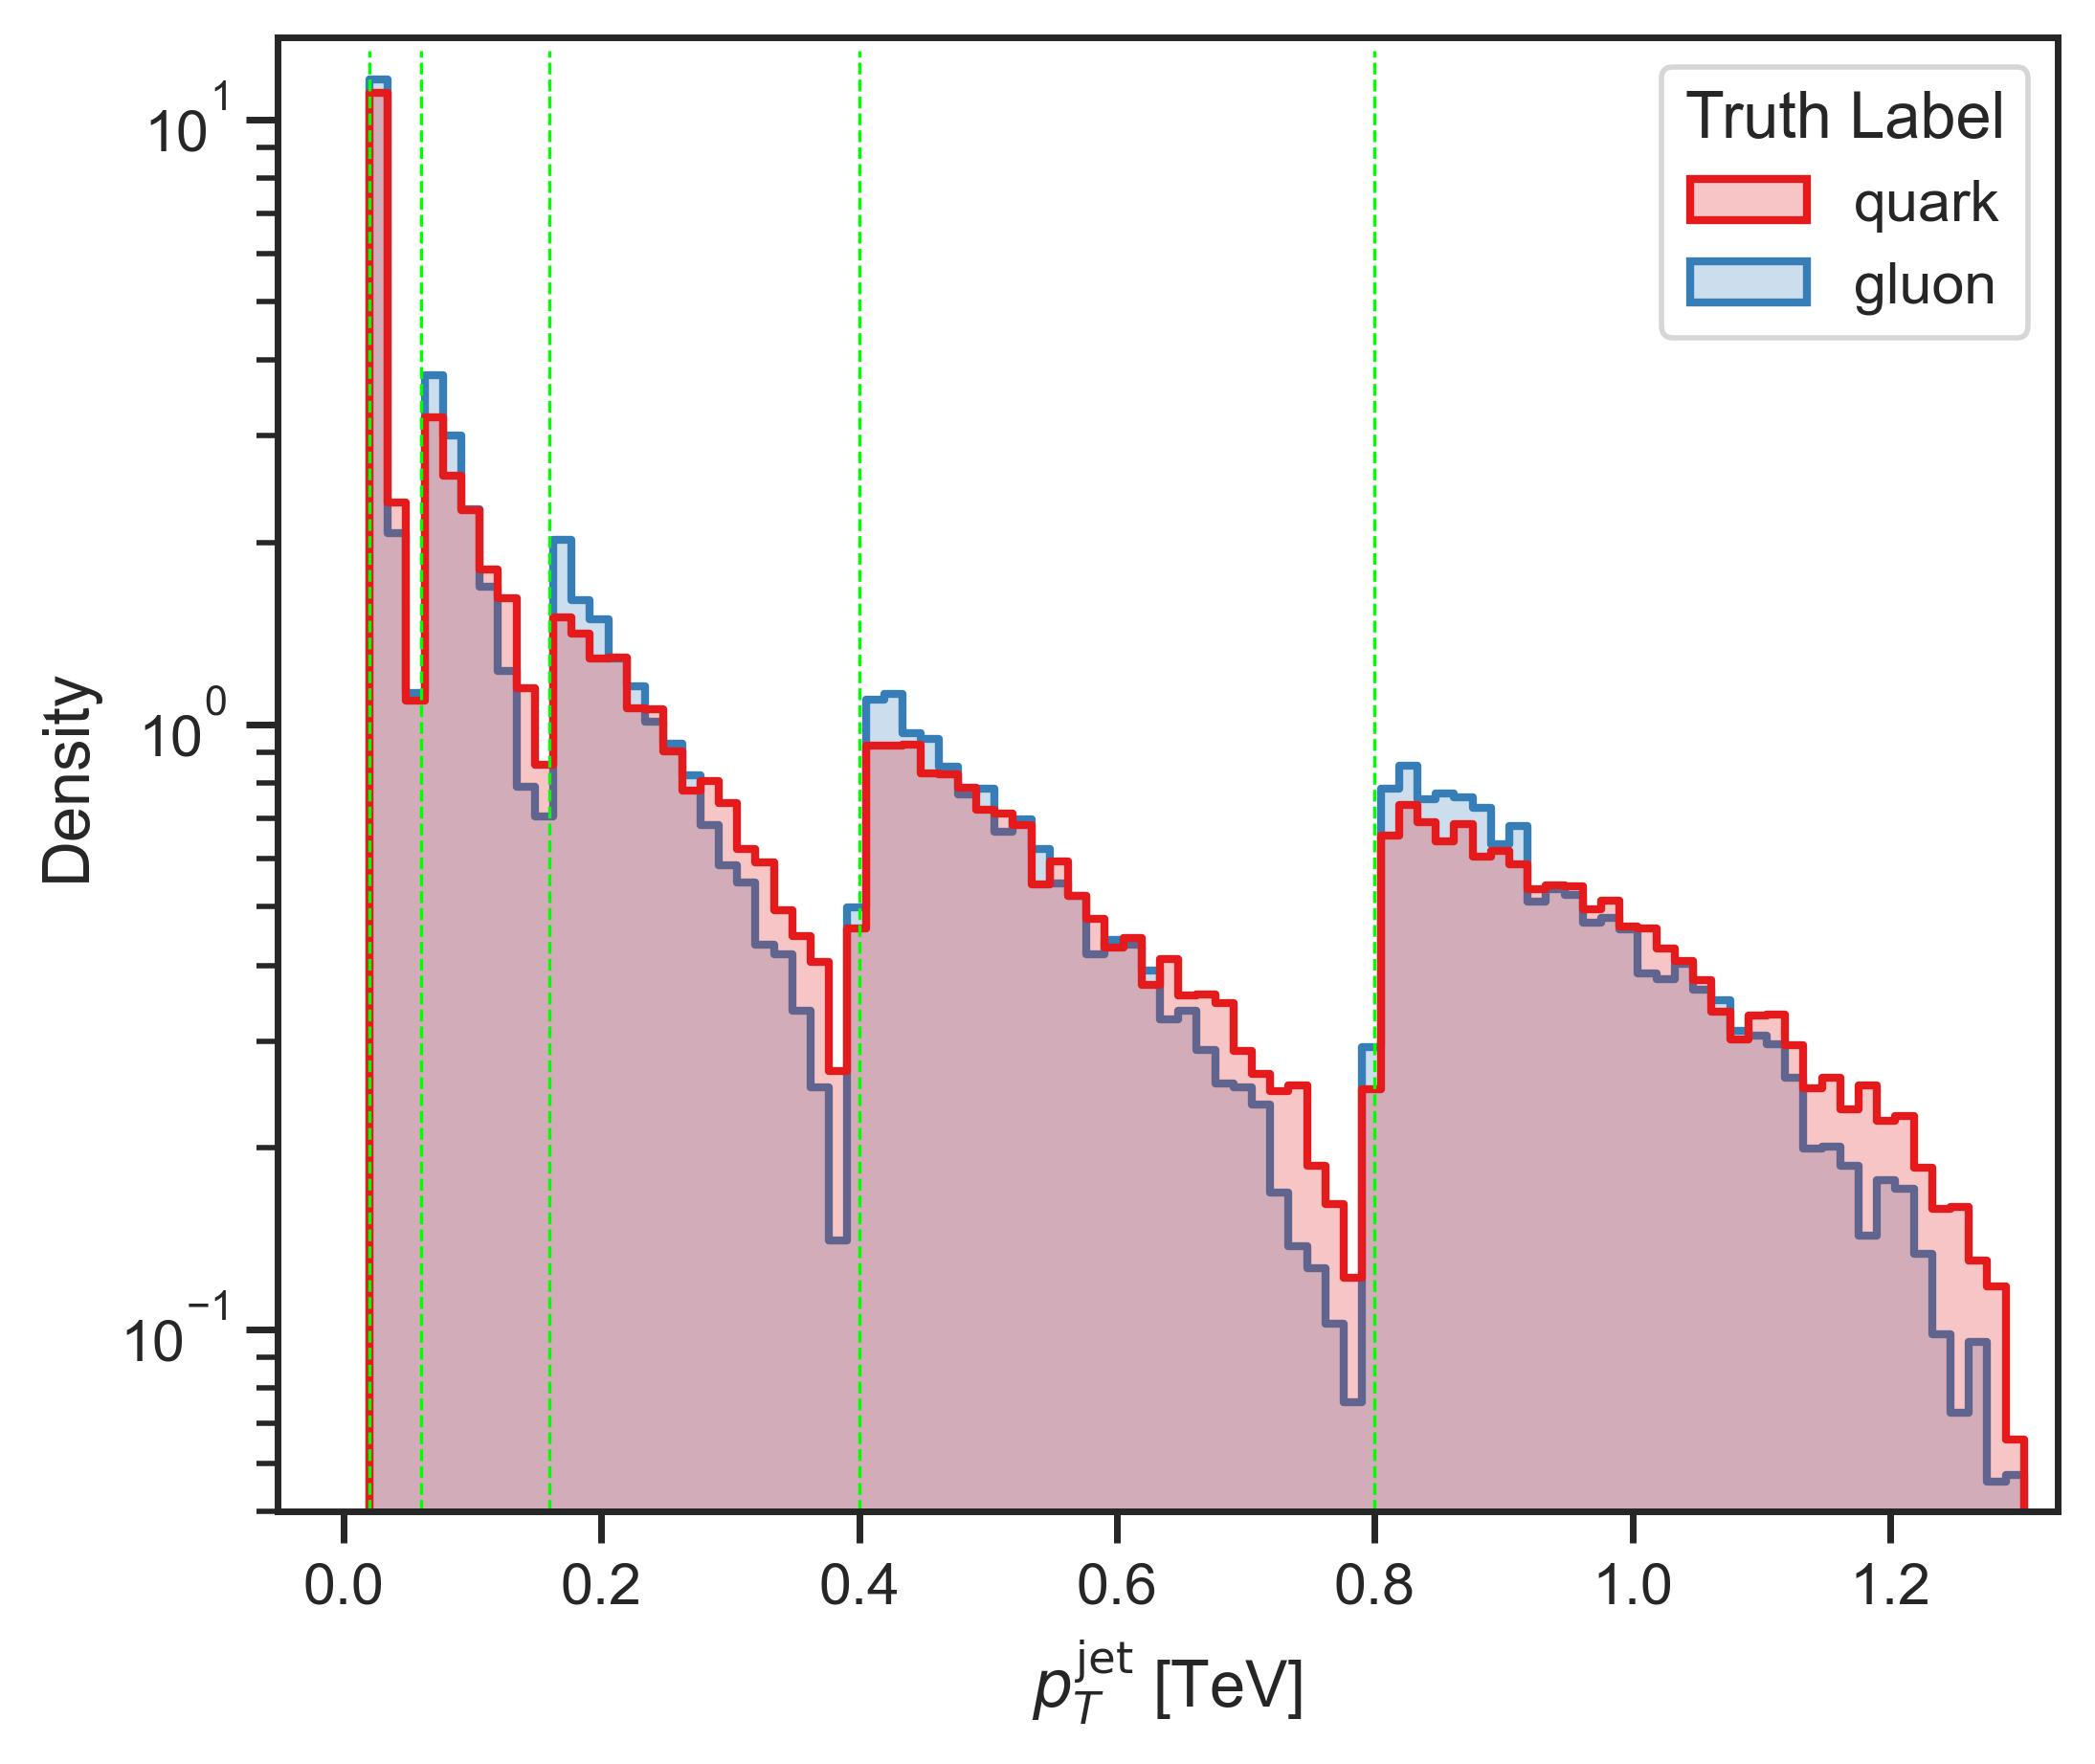
\includegraphics[width=\linewidth]{src/plots/pt_jet_label_cut.jpg}
        \caption{colored by their Truth Label}
        \label{fig:jz_all_cut_label}
    \end{subfigure}
    \begin{subfigure}[t]{0.49\textwidth}
        \centering
        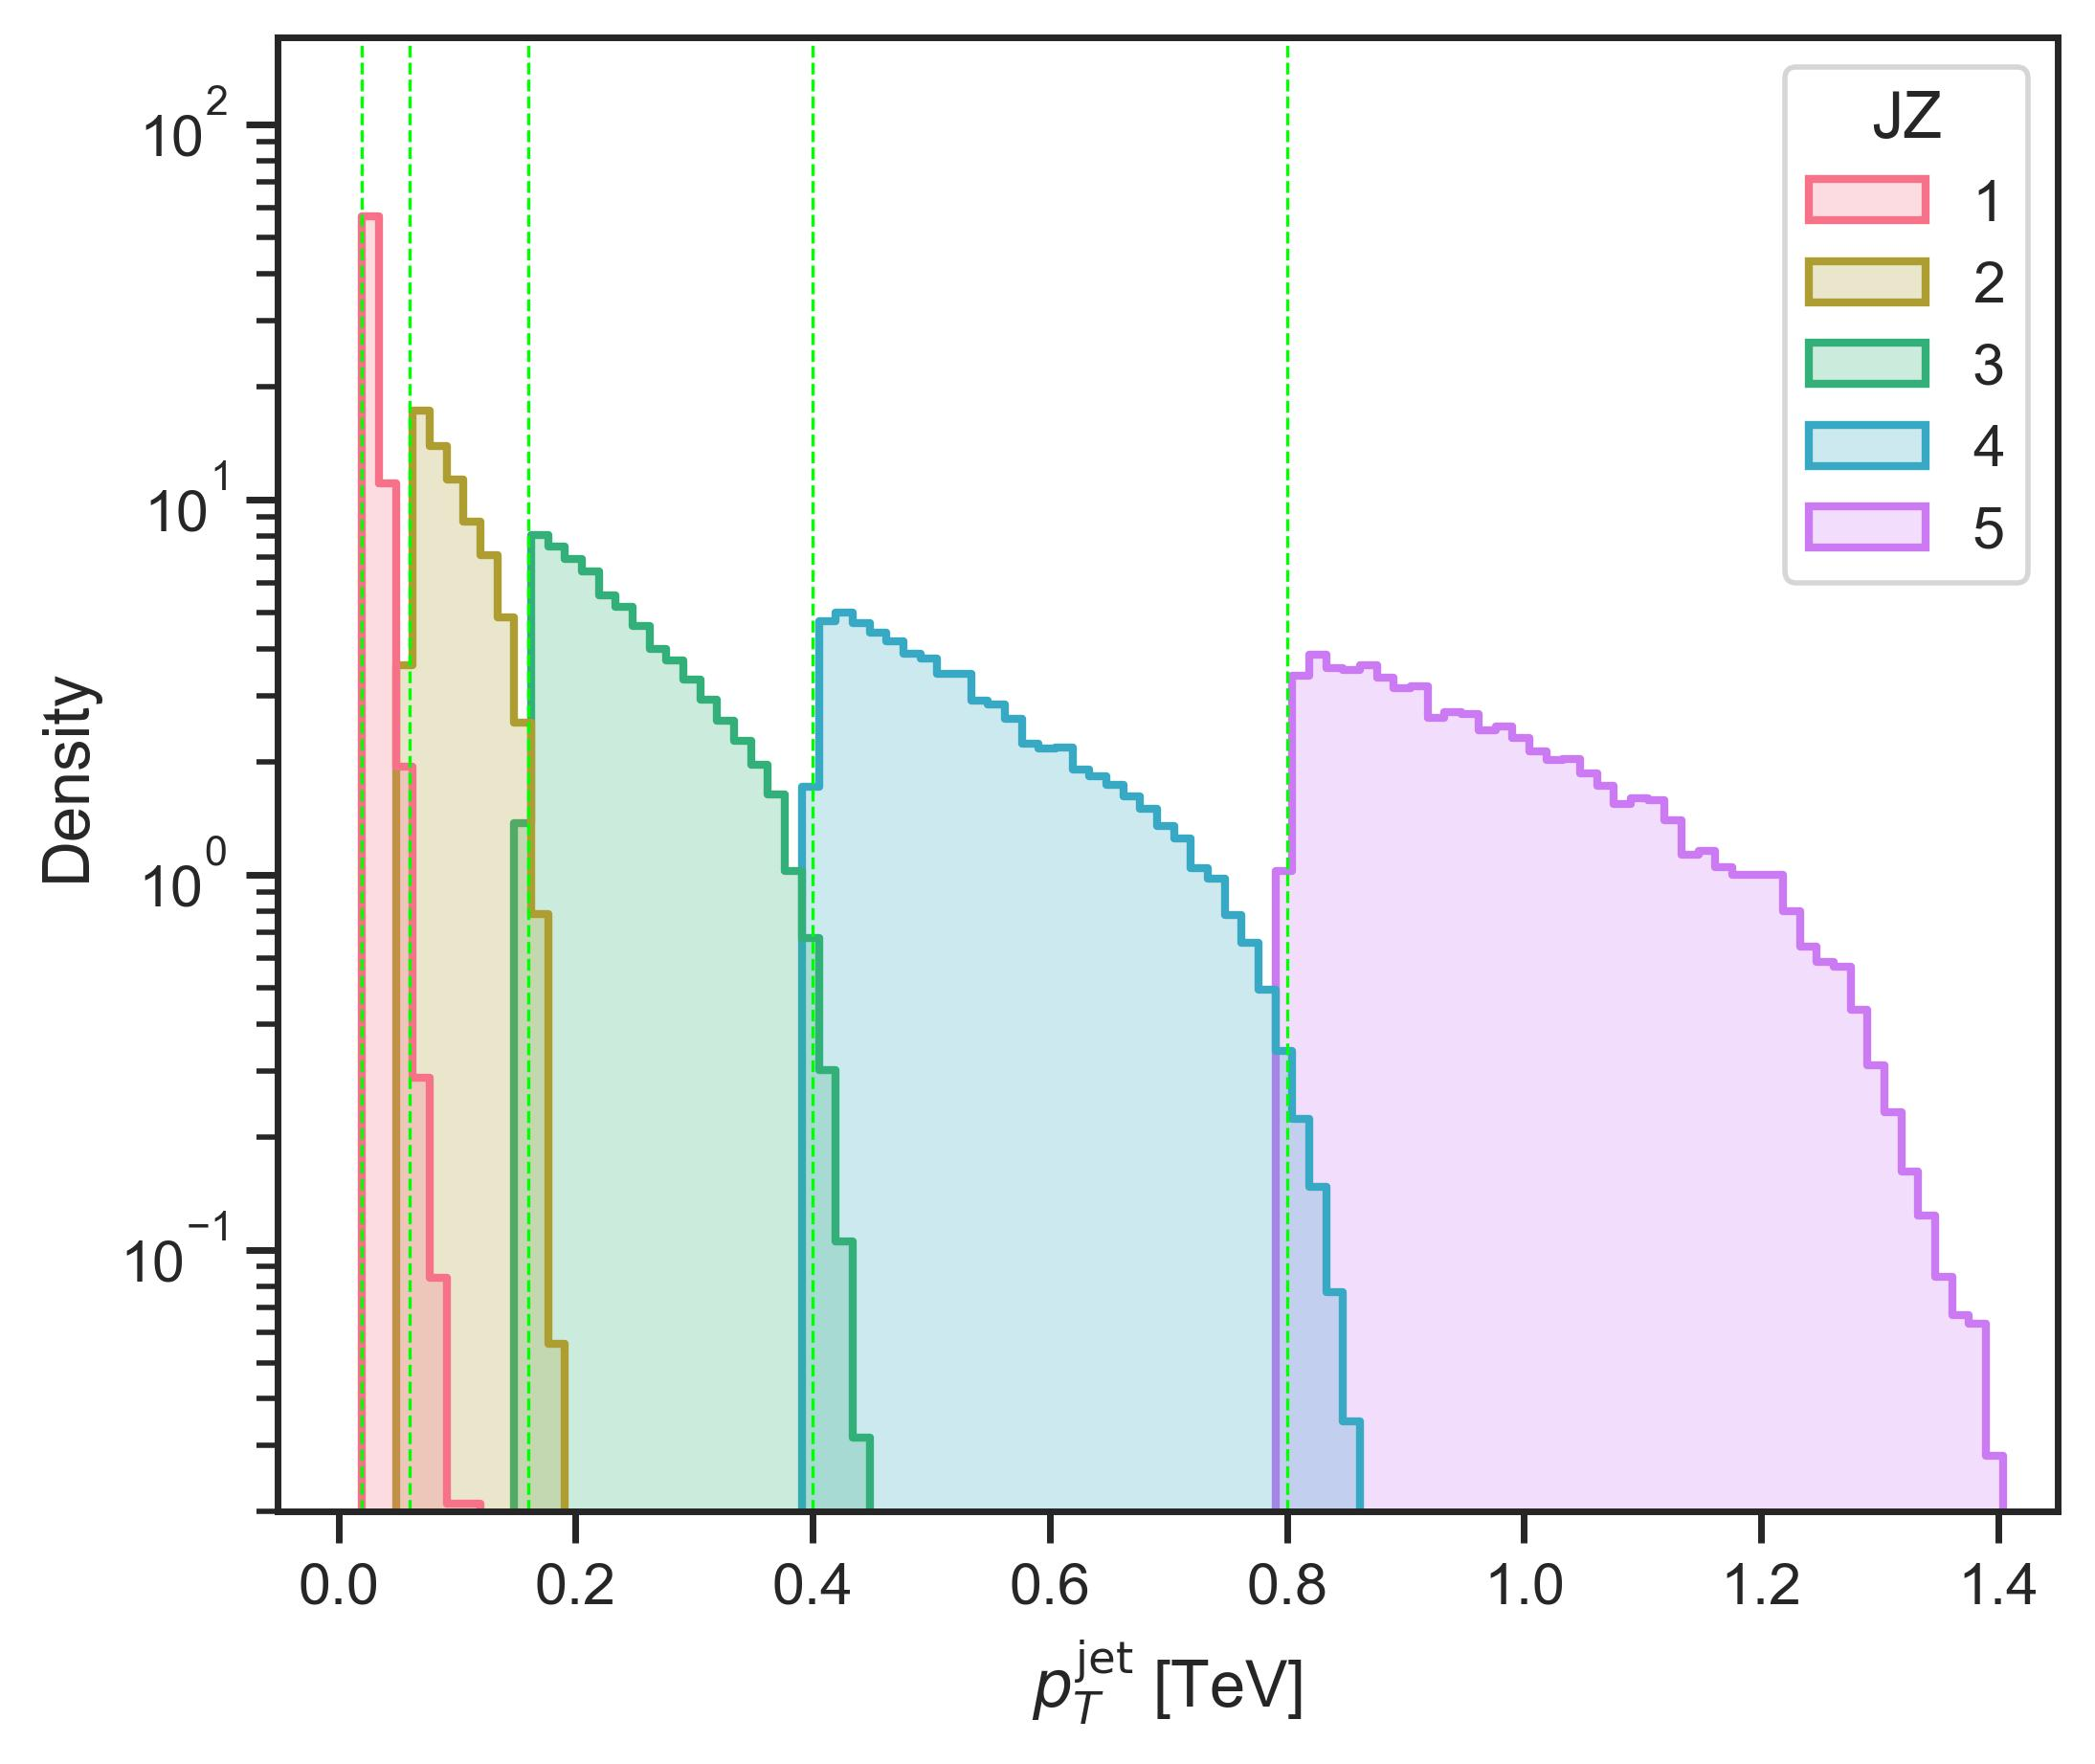
\includegraphics[width=\linewidth]{src/plots/pt_jet_jz_cut.jpg}
        \caption{colored by their JZ slice}
        \label{fig:jz_all_cut_jz}
    \end{subfigure}
    \caption{Normalized $\pT$ distributions of jets after the JZ cuts are applied. Lime lines correspond to the $\pT$ cuts.}
    \label{fig:jz_all_cut}
\end{figure}
We do not want the tagger to use the variable $\pT^{\text{jet}}$ to distinguish between quarks and gluons and avoid jets created from soft gluons.
We separately apply a cut on the jet $\pT$ for each JZ slice.
These cuts are visualized in \cref{fig:jz_separete} with their respective values.
Every jet with lower $\pT$ than the cut is removed from the dataset.

The $\pT$ distributions of the jets after the cuts are applied are shown in \cref{fig:jz_all_cut}.
Contributions from individual JZ slices are also visible in \cref{fig:jz_all_cut_label}, forming a 'cone-line' distribution shape.
The respective cuts are shown with lime lines to make it easier to see the cuts.
The soft gluons are suppressed, and the $\pT$ distribution of the jets is more similar for each Truth Label. 


\FloatBarrier
\section{Input Variables}
\label{sec:input_variables}
We will construct four types of variables:
\begin{itemize}
    \item \textbf{BDT variables} - variables that are calculated from \PFOs for a whole jet.
    \item \textbf{High-level jet variables} - variables that are calculated for the jet.
    \item \textbf{\PFO variables} - variables that are variations of the 4-momenta of the \PFOs, they are calculated for \emph{each PFO} in a given jet.
    \item \textbf{\PFO interaction variables} - variables that are calculated from a pair of 4-momenta of \PFO, they are calculated \emph{for each pair of PFOs} in a given jet.
\end{itemize}
The distributions of these variables are shown in \cref{ch:app_input_variables}

\subsection{PFO Variables}
\label{sec:pfo_variables}
\begin{table}[!htb]
    \centering
    \caption{}
    \label{tab:pfo_variables}
    \begin{tabular}{l}
    \toprule
        PFO Variables \\
    \midrule
        $\Delta \eta = \eta - \eta_\mathrm{jet}$ \\
        $\Delta \phi = \phi - \phi_\mathrm{jet}$ \\
        $\log{p_\mathrm{T}}$ \\
        $\log{\frac{p_\mathrm{T}}{p_\mathrm{T, jet}}}$ \\
        $\log{E}$ \\
        $\log{\frac{E}{E_\mathrm{jet}}}$ \\
        $m$ \\
        $\Delta R = \sqrt{\Delta \eta^2 + \Delta \phi^2}$ \\
    \bottomrule
    \end{tabular}
\end{table}
    
The complete list of \PFO variables is shown in \cref{tab:pfo_variables} \cite{part}.
They are calculated for each \PFO in a given jet.
An input is then a vector of \PFO variables for each \PFO in a given jet, forming an input shape of $N \times 6$, where $N$ is the number of \PFOs in a jet.

We want the tagger to be rotationally invariant, so we only use angles information wrt. the jet axis.
These are the first three variables in \cref{tab:pfo_variables}.
The dynamical variables include the $\pT$ and $E$ of the \PFO.
Long-tailed distributions may cause problems for the neural network, so the logarithms of $\pT$ and $E$ are better suited. 
To emphasize the importance of a given \PFO in a jet, the logarithm of the ratios of $\pT$ ($E$) of a \PFO to a jet $\pT^\mathrm{jet}$ ($E^\mathrm{jet}$) are used.
Most of the \PFOs are assigned zero masses since they are reconstructed as photons.
However, some leave tracks and are reconstructed as charged pions with non-zero masses.
We utilize this information by adding the mass as a variable, which is not used in \cite{part}.

These variables are inputted to \trans, \ParT, and \depart.
\PFN and \EFN also use these variables, apart from the mass $m$.

\subsection{PFO Interaction Variables}
\label{sec:pfo_interaction_variables}
\begin{table}[!htb]
    \centering
    \caption{Interaction PFO variables used as an input to interacting constituent-based models. $E^a$ and $E^b$ are the energies of the two PFOs, $p^{\mu, a}$ and $p^{\mu, b}$ are the 4-momenta of the two PFOs, $\eta^a$ and $\eta^b$ are the pseudorapidities of the two PFOs, $\phi^a$ and $\phi^b$ are the azimuthal angles of the two PFOs, and $p_\mathrm{T}^a$ and $p_\mathrm{T}^b$ are the transverse momenta of the two PFOs. \cite{part}}
    \label{tab:pfo_interaction_variables}
    \begin{tabular}{l}
    \toprule
        PFO Interaction Variables \\
    \midrule
        $\log \Delta = \log{\sqrt{(\eta^a - \eta^b)^2 + (\phi^a - \phi^b)^2}}$ \\
        $\log k_\mathrm{T} = \log{(\min{(p_\mathrm{T}^a, p_\mathrm{T}^b)} \Delta)}$ \\
        $z = \min{(p_\mathrm{T}^a, p_\mathrm{T}^b)}/(p_\mathrm{T}^a + p_\mathrm{T}^b)$ \\
        $\log m^2 = \log{(p^{\mu, a} + p^{\mu, b})^2}$ \\
    \bottomrule
    \end{tabular}
\end{table}
    
The complete list of \PFO interaction variables is shown in \cref{tab:pfo_interaction_variables} \cite{part}.
They are calculated for each pair of \PFOs in a given jet.
An input is a matrix of \PFO interaction variables for each pair of \PFOs in a given jet, forming an input shape of $N \times N \times 6$, where $N$ is the number of \PFOs in a jet.
The matrix is symmetric, and the diagonal is filled with zeros.

The kinematic variable is the angular distance $\Delta$.
The invariant mass $m^2$ is calculated from the 3-momenta of the two \PFOs and their energies.
We utilize the same variable $k_\mathrm{T}$ as used in the jet reconstruction \cref{sec:jet_reco} (however, it is labeled differently, according to \cite{part}).
The last variable, $z$, is also dynamic, the fraction of $\pT$ carried by less energetic \PFO.
Again we take the \emph{logarithm of all these variables} to squish the distributions. 

These variables are a secondary input to \ParT and \depart.
We will train these models both with and without interaction variables.
Those trained with interaction variables are denoted as \emph{Interacting ParT} and \emph{Interacting DeParT}, respectively.

\subsection{BDT Variables}
\label{sec:bdt_variables}
\begin{table}[!htb]
    \centering
    \caption{BDT variables used as an input to the Boosted Decision Tree. $p_\mathrm{T}$ is the transverse momentum of the PFO, $\eta$ is the pseudorapidity of the PFO, $\phi$ is the azimuthal angle of the PFO,  $\eta^{\text{jet}}$ is the pseudorapidity of the jet, and $\phi^{\text{jet}}$ is the azimuthal angle of the jet, $\pT^\mathrm{jet}$ is the transverse momentum of the jet. Summations are over PFOs in the jet. \cite{bdt_tag}}
    \label{tab:bdt_variables}
    \begin{tabular}{l}
    \toprule
        BDT Variables \\
    \midrule
        $p_\mathrm{T}^\mathrm{jet}$ \\
        $\eta^\mathrm{jet}$ \\
        \vspace{1em}
        $N_{\text {PFO}}=\sum_{\text {PFO } \in \text { jet }}$ \\
        \vspace{1em}
        $W_{\text {PFO}}=\frac{\sum_{a \in \mathrm{jet}} p_{\mathrm{T}}^{a} \sqrt{(\eta^a - \eta^{\text{jet}})^2 + (\phi^a - \phi^{\text{jet}})^2}}{\sum_{a \in \mathrm{jet}} p_{\mathrm{T}}^{a}}$ \\
        \vspace{1em}
        $C_1^{\beta=0.2}=\frac{\sum_{a, b \in \mathrm{jet}}^{a \neq b} p_{\mathrm{T}}^a p_{\mathrm{T}}^b \left(\sqrt{(\eta^a - \eta^b)^2 + (\phi^a - \phi^b)^2}\right)^{\beta=0.2}}{\left(\sum_{a \in \mathrm{jet}} p_{\mathrm{T}}^{a}\right)^2}$ \\
    \bottomrule
    \end{tabular}
\end{table}
    
The complete list of BDT variables is shown in \cref{tab:bdt_variables} \cite{bdt_tag} \footnote{In the original paper \cite{bdt_tag}, they do not use \PFOs, but only track (trk) information.}.
They are calculated for the whole jet from all \PFOs, forming a 5-dimensional vector as an input.

$N_\mathrm{PFO}$ is the number of \PFOs in a jet, i.e. the \emph{multiplicity}.
Before \bdt, taggers used this single variable to tag jets. 
Variables $W_\mathrm{PFO}$ and $C_1^{\beta = 1}$ are carefully engineered to achieve the best performance.
The $\pT^{\text{jet}}$ and $\eta^\mathrm{jet}$ were only added in the last version of the tagger \cite{bdt_tag}.

Only \bdt uses these variables as input.

\subsection{High-level Jet Variables}
\label{sec:high_level_variables}
\begin{table}[!htb]
    \centering
    \small
    \caption{High-level jet variables commonly used in ATLAS analyses. They come precomputed by \texttt{Athena} in the jet container. Index 0 refers to the first entry of that variable in the jet container.}
    \label{tab:high_level_variables}
    \begin{tabular}{ll}
    \toprule
    \normalsize{High-level Jet Variables} &  \\
    \midrule
        \texttt{ActiveArea4vec\_(m,pt,eta,phi)} & \texttt{fJVT}\\
        \texttt{JetConstitScaleMomentum\_(m,pt,eta,phi)} & \texttt{passFJVT}\\
        \texttt{averageInteractionsPerCrossing[0]} & \texttt{Jvt}\\
        \texttt{FracSamplingMax} & \texttt{JvtRpt}\\
        \texttt{FracSamplingMaxIndex} & \texttt{passJVT}\\
        \texttt{GhostMuonSegmentCount} & \texttt{JVFCorr}\\
        \texttt{ChargedPFOWidthPt1000[0]} & \texttt{Timing}\\
        \texttt{TrackWidthPt1000[0]} & \texttt{EMFrac}\\
        \texttt{NumChargedPFOPt1000[0]} & \texttt{Width}\\
        \texttt{NumChargedPFOPt500[0]} & \texttt{chf}\\
        \texttt{SumPtChargedPFOPt500[0]} & \texttt{PFO\_n}\\
        \texttt{(m,pt,eta,phi)} & \\
        \bottomrule
    \end{tabular}
\end{table}
    


The complete list of high-level jet variables is shown in \cref{tab:high_level_variables}, and their definitions and commonly used symbols are given in \cref{ch:app_high_level_variables}.
These variables are precomputed by the \texttt{Athena} \footnote{https://atlassoftwaredocs.web.cern.ch/athena/athena-releases/} framework and are available for each jet.
Together they form a 30-dimensional vector as an input.

\fc and \highway use these variables as input.

\subsection{Normalization}
\label{sec:input_normalization}
To make the learning process easier, we normalize the input variables.
This helps the neural network to converge faster and avoids numerical problems.
Only \bdt variables are not normalized since \bdt performance is not affected by the normalization.

We can sketch the normalization procedure as follows:
\begin{equation}
    \xi \rightarrow \tilde{\xi} = \frac{\xi - \mu}{\sigma},
\end{equation}
where $\xi$ is the input variable, $\mu$ is the mean of the variable, and $\sigma$ is the standard deviation of the variable.
Each variable is normalized separately, shifting the mean to zero and squishing the distribution to unit variance.

The mean and standard deviation are precomputed on a subset of the data before training.
We utilize the \texttt{tf.keras.layers.Normalization}\footnote{\url{https://www.tensorflow.org/api_docs/python/tf/keras/layers/Normalization}} with \texttt{axis=-1}, and the method \texttt{adapt} to compute the mean and standard deviation.
Means and standard deviations are fixed, \emph{untrainable parameters}.


\section{Training Configuration}
\label{sec:training_config}
\begin{table}[h]
    \centering
    \caption{Summary of common training configuration for all models.}
    \label{tab:training_config}
    \begin{tabular}{@{}lc@{}}
        \toprule
        \multicolumn{2}{c}{\textbf{Data}} \\
        \midrule
        Training Dataset & 5M jets \\
        Validation Dataset & 0.5M jets \\
        Test Dataset & 0.5M jets \\
        Number of Epochs & 12 \\
        Batch Size & 512 \\
        Total Steps & 118k \\
        Normalization Layer & adaptation on 500 batches \\
        \midrule
        \multicolumn{2}{c}{\textbf{Optimizer}} \\
        \midrule
        Optimizer & LAMB \\
        Learning Rate & 0.001  \\
        $\beta_1$ & 0.9 \\
        $\beta_2$ & 0.999 \\
        $\epsilon$ & $10^{-6}$ \\
        Learning Rate Scheduling & Cosine Decay \\
        Warmup & Linear (100 steps) \\
        Clip Norm & None \\
        \midrule
        \multicolumn{2}{c}{\textbf{Loss}} \\
        \midrule
        Loss & Binary Cross Entropy \\
        Label Smoothing & None \\
        Weight Decay & None \\
        \bottomrule
        \end{tabular}
        \end{table}
        
        
        
    
The training is performed with \texttt{TensorFlow 2.9.1} \cite{tf} and \texttt{Keras 2.9.0} \cite{keras}.
The general training configuration is the same for all models, with some exceptions for \bdt.
The training dataset consists of \textbf{5M jets}.
The validation and test datasets both consist of 0.5M jets.
Each model is trained for \textbf{12 epochs} (except \bdt, which has no epochs) with a \textbf{batch size of 512} (resulting in 118K steps).
Validation is performed after each epoch, calculating the AUC and Accuracy.
We employ the \textbf{LAMB optimizer} (with $\beta_1= 0.9$, $\beta_2= 0.999$, $\epsilon= 10^{-6}$) with an initial learning rate of 0.001, \textbf{cosine-decaying} to zero over the 12 epochs.
No clipnorm nor weight decay is used, but a \textbf{linear warmup} is applied for the first 100 steps of the training.
We utilize the \textbf{binary cross-entropy} loss function without label smoothing.
We use 500 batches to calculate the mean and standard deviation for the normalization layer.
Hyperparameters are summarized in \cref{tab:training_config}.
There was no extensive hyperparameter tuning. 
They were chosen based on related works \cite{deit3,part,cait,bert}.

All models have approximately \textbf{2.6M parameters}, except \bdt.
There were trained on two \texttt{NVIDIA TESLA V100} GPUs with 16GB or 32GB of memory (depending on the model, interaction variables are more memory-hungry).

\subsection{BDT Configuration}
\label{sec:bdt_config}
\begin{table}[htb]
    \centering
    \caption{Configuration of BDT model.}
    \label{tab:bdt_config}
    \begin{tabular}{@{}lc@{}}
    \toprule
    \textbf{Parameter} & \textbf{BDT} \\ \midrule
    Number of Trees & 600 \\
    Growing Strategy & \texttt{BEST\_FIRST\_GLOBAL} \\
    Maximum Depth & 5 \\
    Split Axis & \texttt{SPARSE\_OBLIQUE} \\
    Shrinkage & 0.5 \\
    Minimum Examples per Leaf & 5k \\
    L2 Regularization & 0.1 \\
    \bottomrule
    \end{tabular}
\end{table}
The training is performed with the \texttt{TensorFlow Decision Forests 0.2.7} \footnote{\url{https://www.tensorflow.org/decision_forests}} library using the \texttt{tfdf.keras.GradientBoostedTreesModel} model.
We train 600 trees with a maximum depth of 5.
The minimum number of samples in a leaf is 5000.
The shrinkage factor is 0.5, and L2 regularization is applied with a weight of 0.1.
The loss is the same as for the neural networks, the binary cross-entropy.
The \texttt{BEST\_FIRST\_GLOBAL} growing policy is used, and the split axis policy is \texttt{SPARSE\_OBLIQUE}.
All additional parameters are set to their default values\footnote{\url{https://www.tensorflow.org/decision_forests/api_docs/python/tfdf/keras/GradientBoostedTreesModel}}.
Everything is summarized in \cref{tab:bdt_config}.

\subsection{Transformer, ParT, and DeParT Configuration}
\label{sec:transformer_config}
\begin{table}[h]
    \centering
    \caption{Configuration of Transformer, ParT, and DeParT models.} 
    \label{tab:trans_config}
    \begin{tabular}{@{}lccc@{}}
    \toprule
    \textbf{Parameter} & \textbf{Transformer} & \textbf{ParT} & \textbf{DeParT} \\ \midrule
    Embedding Dimension & 128 & 128 & 128 \\
    Self-Attention Block Layers & 13 & 11 & 11 \\
    Class Attention Block Layers & - & 2 & 2 \\
    Heads & 8 & 8 & 8 \\
    Expansion & 4 & 4 & 4 \\
    Dropout & - & 0.1 & - \\
    Stochastic Depth Drop Rate & - & - & 0.1 \\
    Layer Scale Initialization & - & - & $10^{-5}$ \\
    Number of Embedding Layers & 3 & 3 & 3 \\
    Number of Interaction Embedding Layers & - & 3 & 3 \\
    Size of Interaction Embedding Layers & - & 64 & 64 \\
    Activation & GELU & GELU & GELU \\
    \bottomrule
    \end{tabular}
    \end{table}
Transformer, \ParT, and \depart embed the input variables into 128 dimensions, with 3 embedding layers.
The total number of layers of each model is 13, where in the case of \depart and \ParT, the last 2 layers are \CA Blocks.
All three models use 8 heads and \FFN expansion factor of 4, which results in 512 dimensions in the \FFN layer and GELU Activation.
In the case of the \trans, no dropout is applied, \ParT uses dropout with a rate of 0.1, and \depart uses Stochastic Depth Drop with a rate of 0.1.
\depart also uses the Layer Scale with an initial value of $10^{-5}$.

\ParT and \depart are trained with and without the interaction variables.
If they are, the interaction variables are embedded with 3 layers, each of size 64, while the last one is the same as the number of heads, 8.
All hyperparameters are summarized in \cref{tab:trans_config}.

\subsection{Fully Connected and Highway Network Configuration}
\label{sec:fc_config}
\begin{table}[h]
    \centering
    \caption{Configuration of FC and Highway models.}
    \label{tab:fc_config}
    \begin{tabular}{@{}lcc@{}}
    \toprule
    \textbf{Parameter} & \textbf{Fully Connected} & \textbf{Highway} \\ \midrule
    Layer Size & 512 & 344 \\
    Number of Layers & 11 & 11 \\
    Dropout & 0.2 & 0.2 \\
    Activation & Swish & Swish \\
    \bottomrule
    \end{tabular}
\end{table}
Both \fc and \highway have 11 hidden layers with a 0.2 dropout rate and Swish Activation.
\fc has 512 neurons in each layer, while \highway has 344 neurons to account for the skip connections.

\subsection{PFN and EFN Configuration}
\label{sec:efn_config}
\begin{table}[h]
    \centering
    \caption{Configuration of PFN and EFN models.}
    \label{tab:pfn_config}
    \begin{tabular}{@{}lcc@{}}
    \toprule
    \textbf{Parameter} & \textbf{PFN} & \textbf{EFN} \\ \midrule
    $\Phi$ layers & 5 x 512 & 4 x 512 + 1 x 136 \\
    $F$ layers & 6 x 512 & 6 x 512 \\
    $\Phi$ & CNN & CNN \\
    Activation & ReLU & ReLU \\
    Dropout & - & - \\
    \bottomrule
    \end{tabular}
\end{table}
Both \PFN and \EFN use \pointCNN for the $\Phi$ mapping. 
\PFN has 5 layers of sizes 512, while \EFN has 4 layers of sizes 512 and one of 136 to account for the summation over the \PFOs while still having roughly the same number of parameters as \PFN.
For the $F$ function, both models use 6 layers of sizes 512. 
All Activation functions are ReLU, and no dropout is applied.


\section{Results}
\label{sec:results}
\begin{table}[!htb]
    \centering
    \caption{Results of the different models. The best results are highlighted in bold.}
    \label{tab:results}
    \begin{tabular}{lcccccc}
    \toprule
        Model & Accuracy & AUC & $\epsilon_q$ & $\epsilon_g$ \\
    \midrule
        Interacting DeParT & \textbf{0.7433} & \textbf{0.8227} & \textbf{0.7204} & 0.7680 \\
        Interacting ParT & 0.7427 & 0.8223 & 0.7142 & 0.7730 \\
        DeParT & 0.7414 & 0.8203 & 0.7163 & 0.7669 \\
        ParT & 0.7404 & 0.8194 & 0.7092 & \textbf{0.7777} \\
        Transformer & 0.7384 & 0.8170 & 0.7138 & 0.7634 \\
        PFN & 0.7366 & 0.8150 & 0.7101 & 0.7661 \\
        EFN & 0.7201 & 0.7966 & 0.6890 & 0.7555 \\
        Highway & 0.7316 & 0.8089 & 0.7017 & 0.7617 \\
        Fully Connected & 0.7306 & 0.8100 & 0.6998 & 0.7620 \\
        BDT & 0.7073 & 0.7823 & 0.6721 & 0.7426 \\
    \bottomrule
    \end{tabular}
\end{table}
    
\begin{table}[!htb]
    \centering
    \caption{Technical information about the models. The total number of parameters is given in millions. The time and memory are measured on a single NVIDIA Tesla V100 GPU 32GB. The time corresponds to the inference time of one batch of size 512. Memory is the maximum GPU memory usage during inference of batch with size 512.}
    \label{tab:tech}
    \begin{tabular}{lccc}
    \toprule
        Model & Params [$10^{6}$] & Batch Time [ms] & GPU Memory [MB] \\
    \midrule
        Interacting DeParT &  2.62 & 190.3 & 2578 \\
        Interacting ParT & 2.62 & 169.7 & 1411 \\
        DeParT &  2.61 & 118.0 & 574 \\
        ParT & 2.61 & 95.8 & 536 \\
        Transformer & 2.61 & 110.0 & 570 \\
        PFN & 2.64 & 15.6 & 359 \\
        EFN & 2.60 & 15.0 & 551 \\
        Highway & 2.62 & 2.8 & 44 \\
        Fully Connected & 2.64 & 1.6 & 34 \\
        BDT &  - & 20.4 & - \\
    \bottomrule
    \end{tabular}
\end{table}
    

The training results are shown in \cref{tab:results}. 
Our proposed \depart model with interaction variables outperforms all other models.
It also outperforms all other models without interaction variables.
What is fascinating is that the previously used model on jet tagging, \bdt, gets obliterated by \emph{all} other models.
However, the differences between the models are not as significant as expected.
This is due to the physical limit of the tagging task at low $\pT$.
We will discuss this in more detail in \cref{sec:pt_dependance}.

The technical information about the models is summarized in \cref{tab:tech}.
The disk space of all models is roughly the same, around 35 MB, except for \bdt, which is 1.4 MB.
It is given by the number of total parameters, which is roughly the same for all models.
The tiny differences did not affect the performance.

\begin{figure}[ht]
    \centering
    \begin{subfigure}[b]{0.49\textwidth}
        \centering
        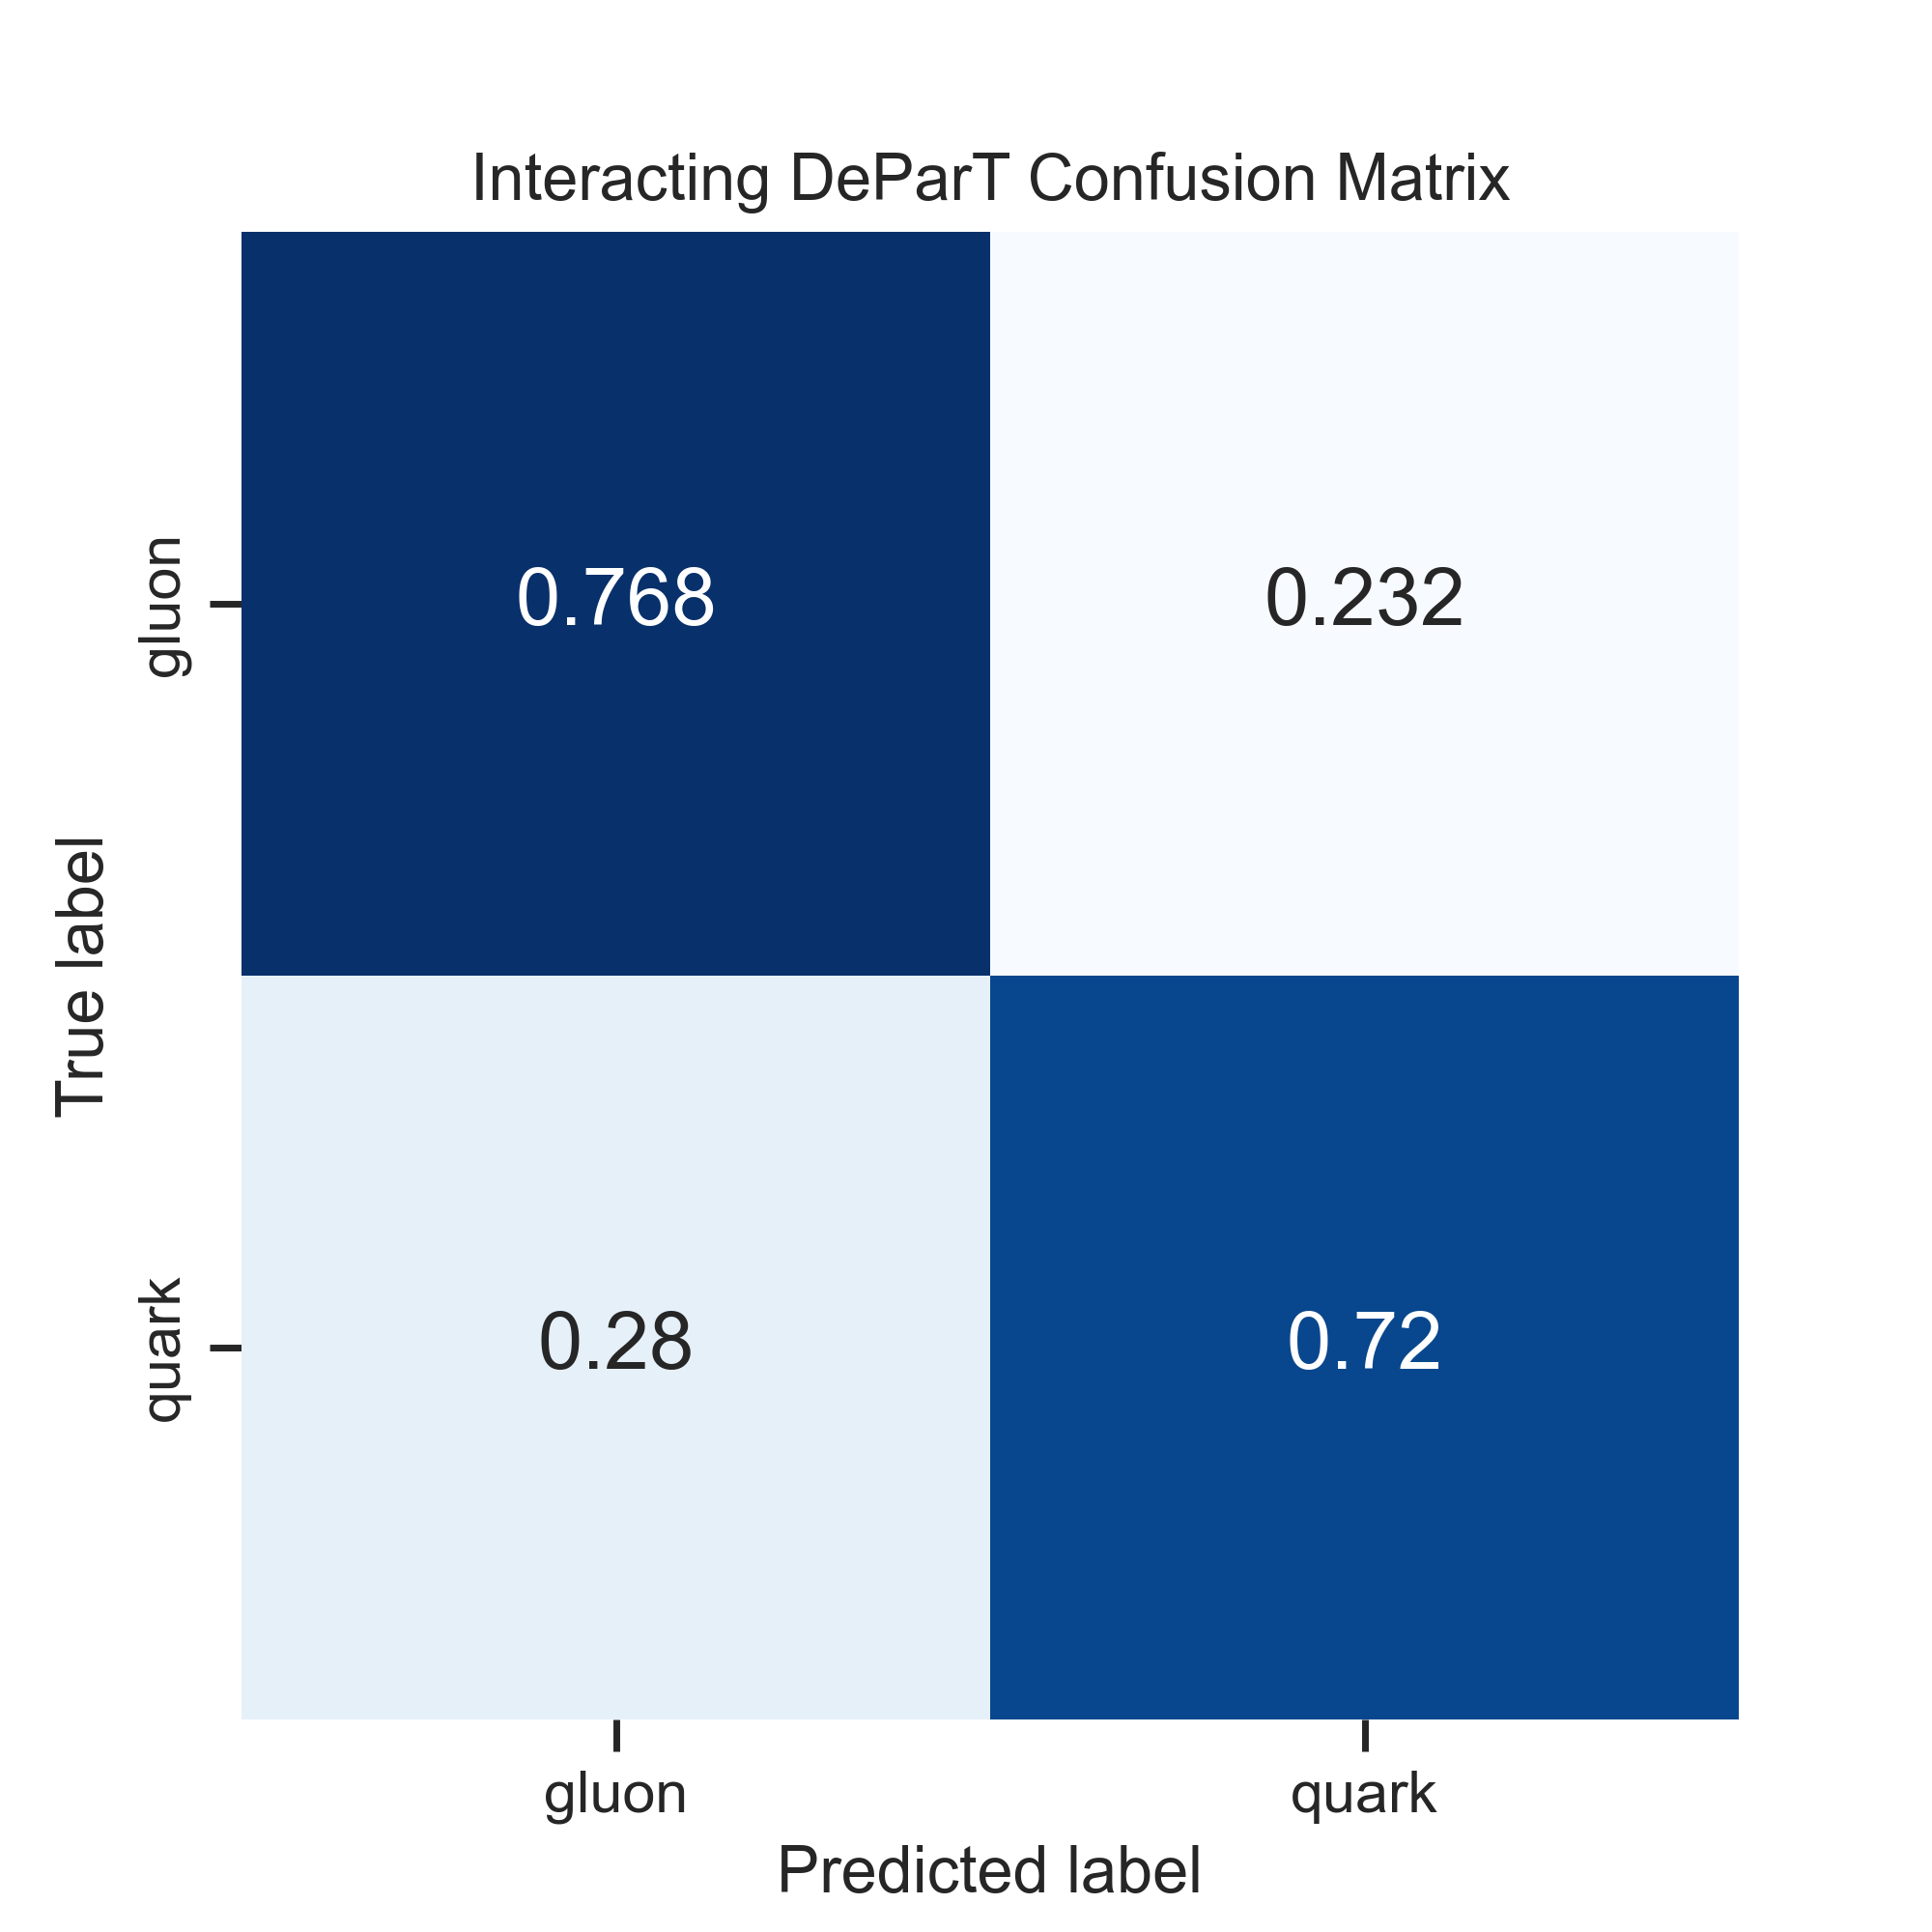
\includegraphics[width=\textwidth]{src/plots/results/cm/interacting_depart.png}
        \caption{Interacting DeParT}
        \label{fig:confusion_depart}
    \end{subfigure}
    % \begin{subfigure}[b]{0.49\textwidth}
    %     \centering
    %     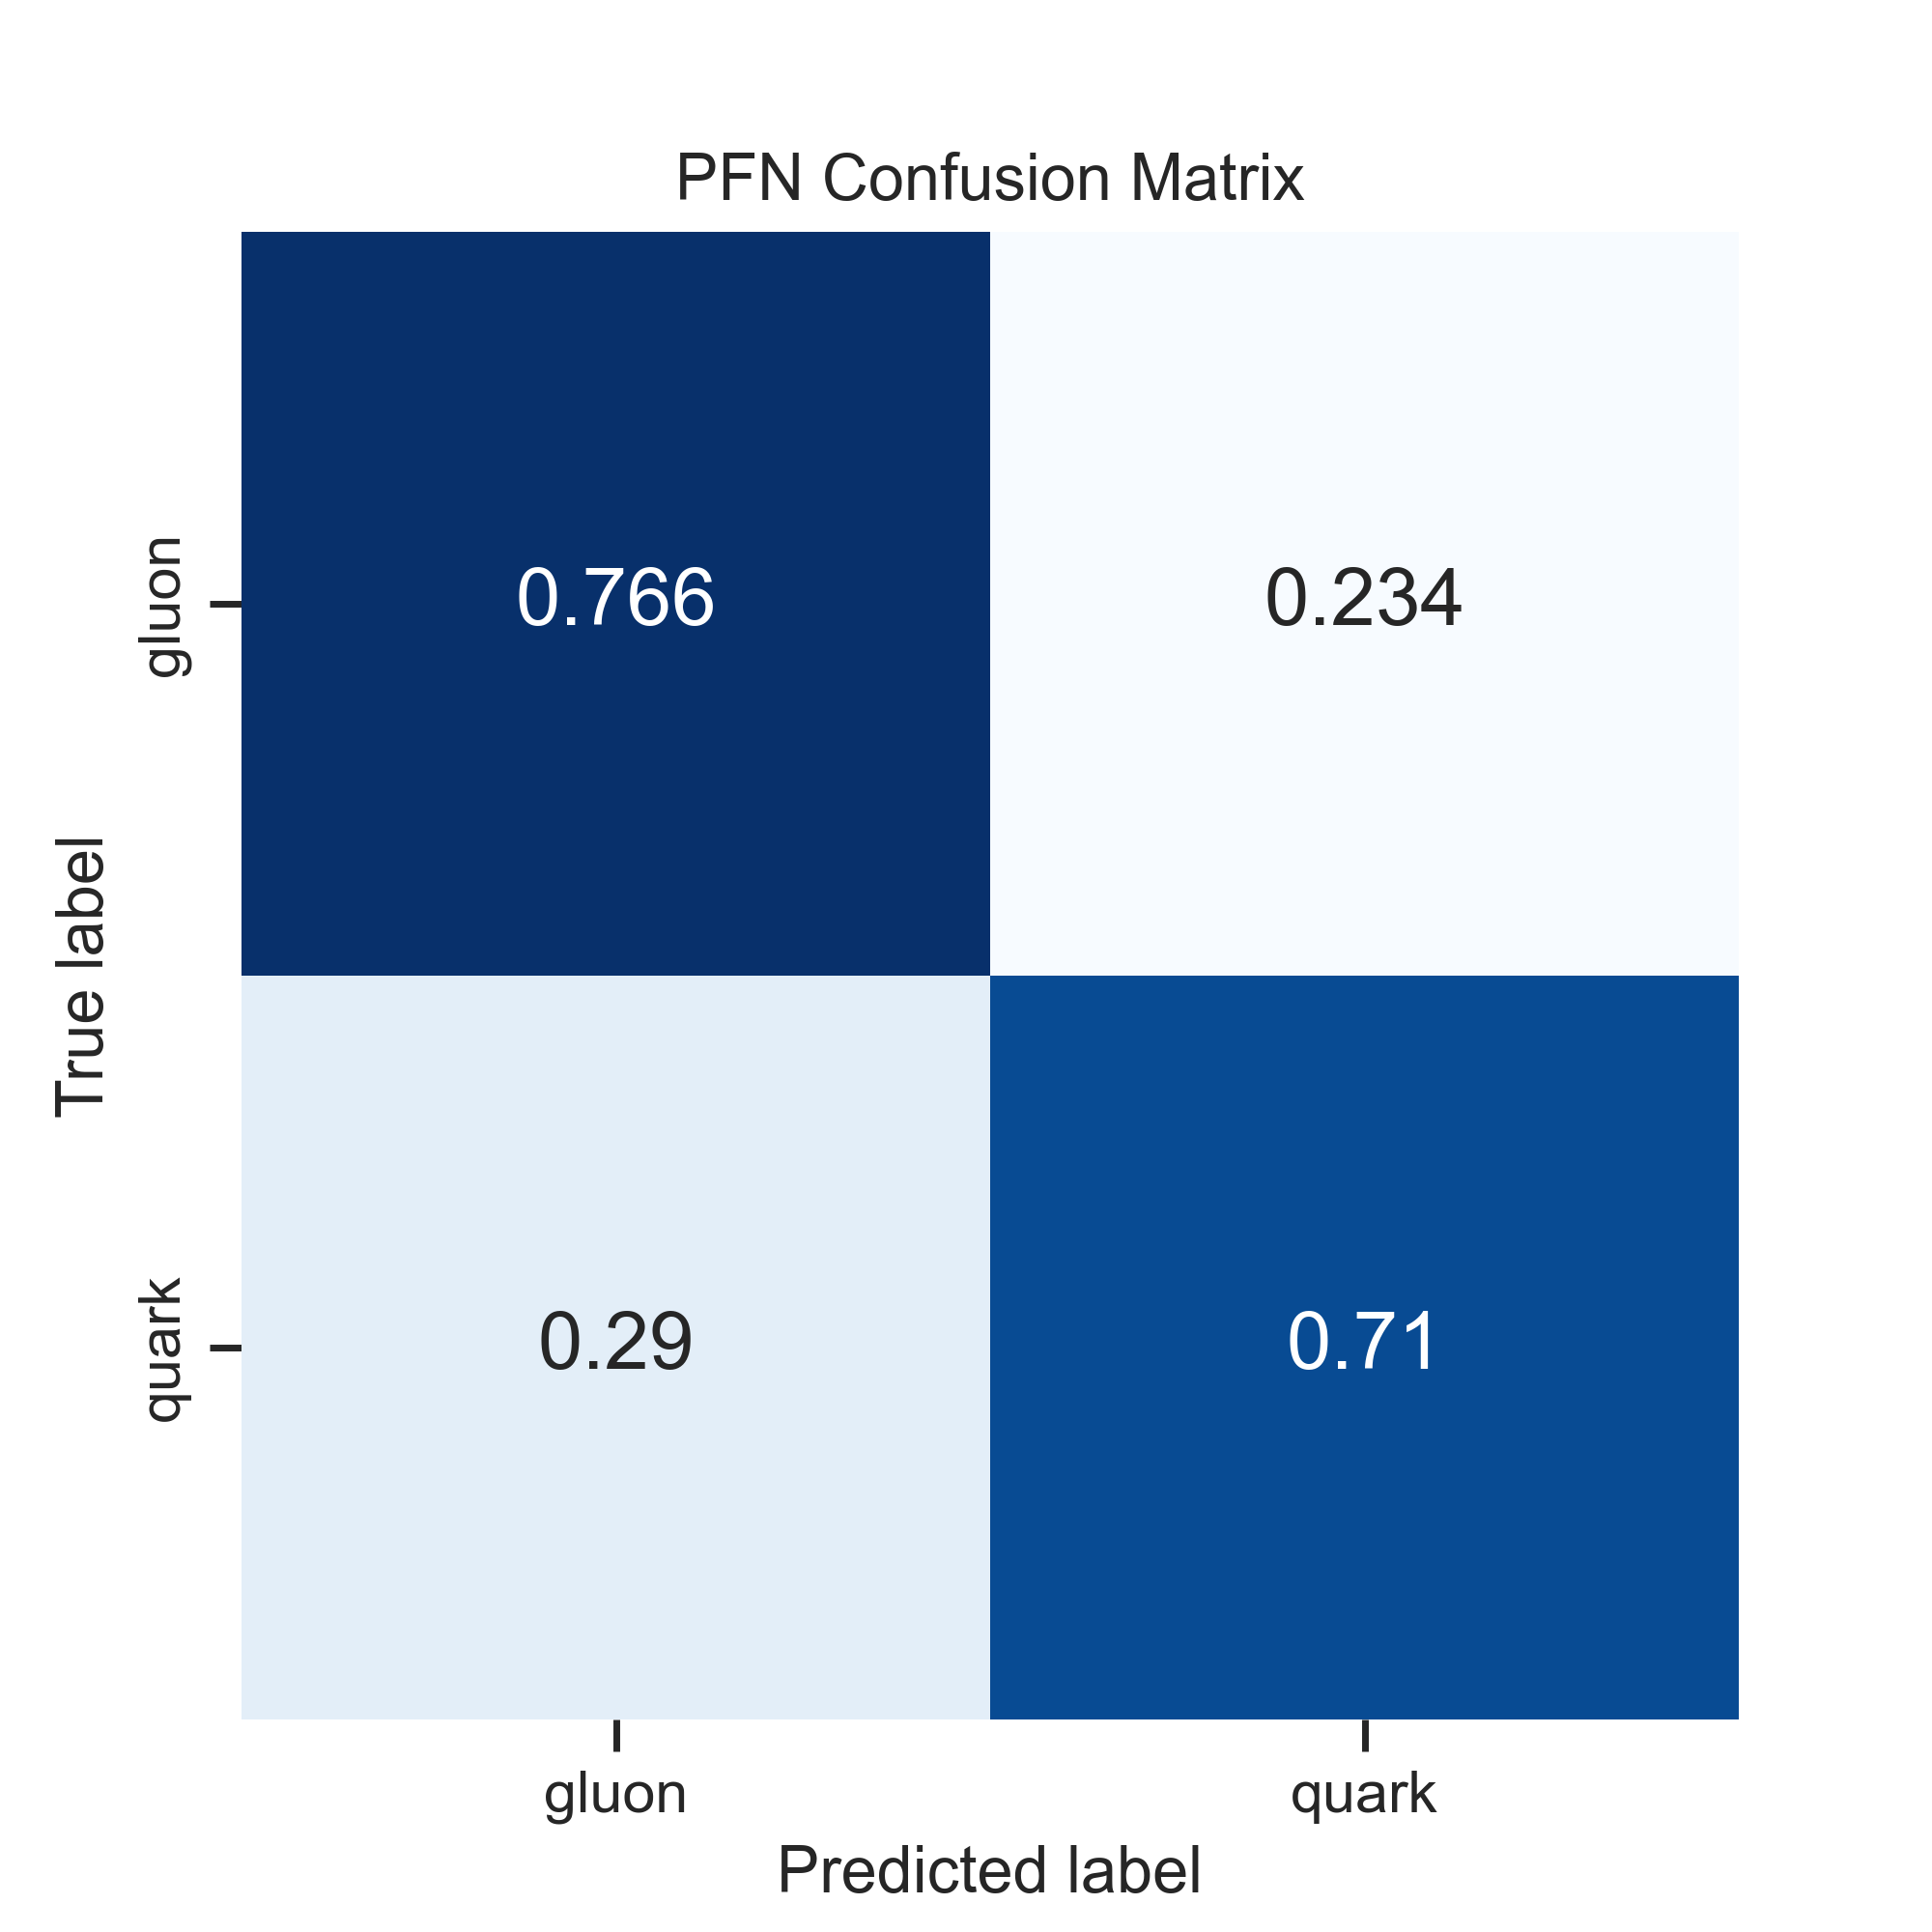
\includegraphics[width=\textwidth]{src/plots/results/cm/pfn.png}
    %     \caption{PFN}
    %     \label{fig:confusion_pfn}
    % \end{subfigure}
    % \begin{subfigure}[b]{0.49\textwidth}
    %     \centering
    %     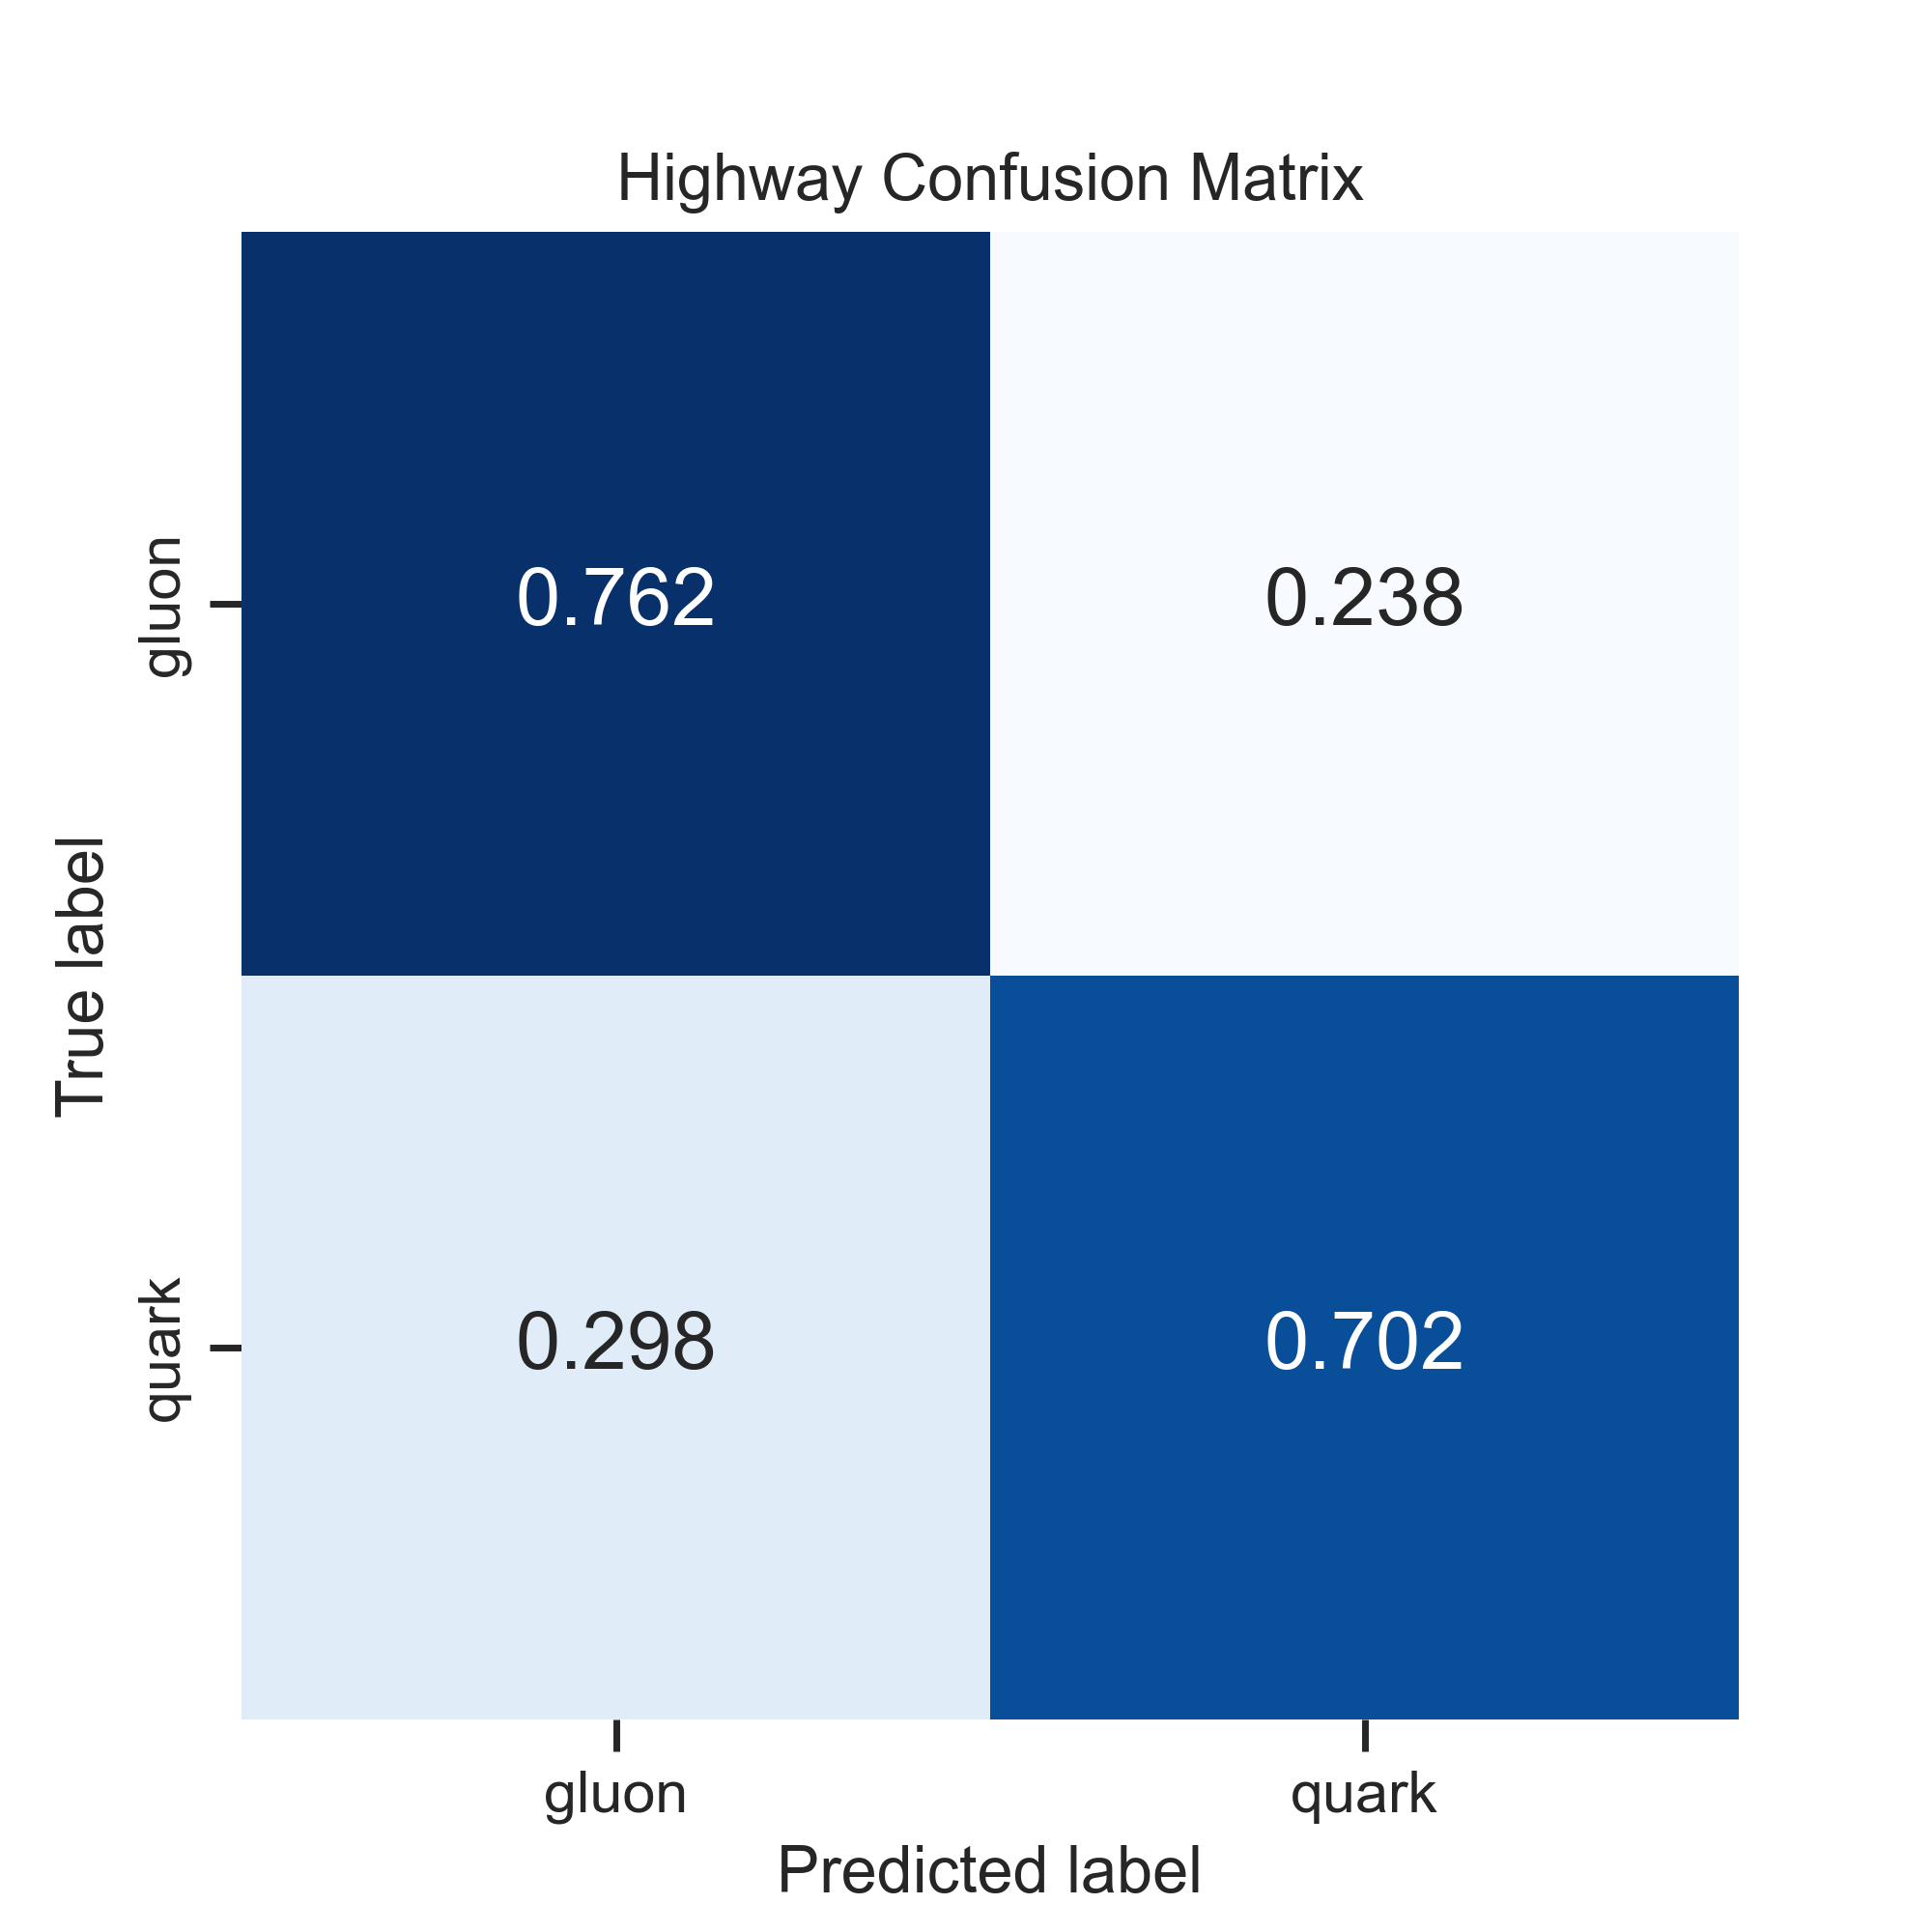
\includegraphics[width=\textwidth]{src/plots/results/cm/highway.png}
    %     \caption{Highway}
    %     \label{fig:confusion_depart_inter}
    % \end{subfigure}
    \begin{subfigure}[b]{0.49\textwidth}
        \centering
        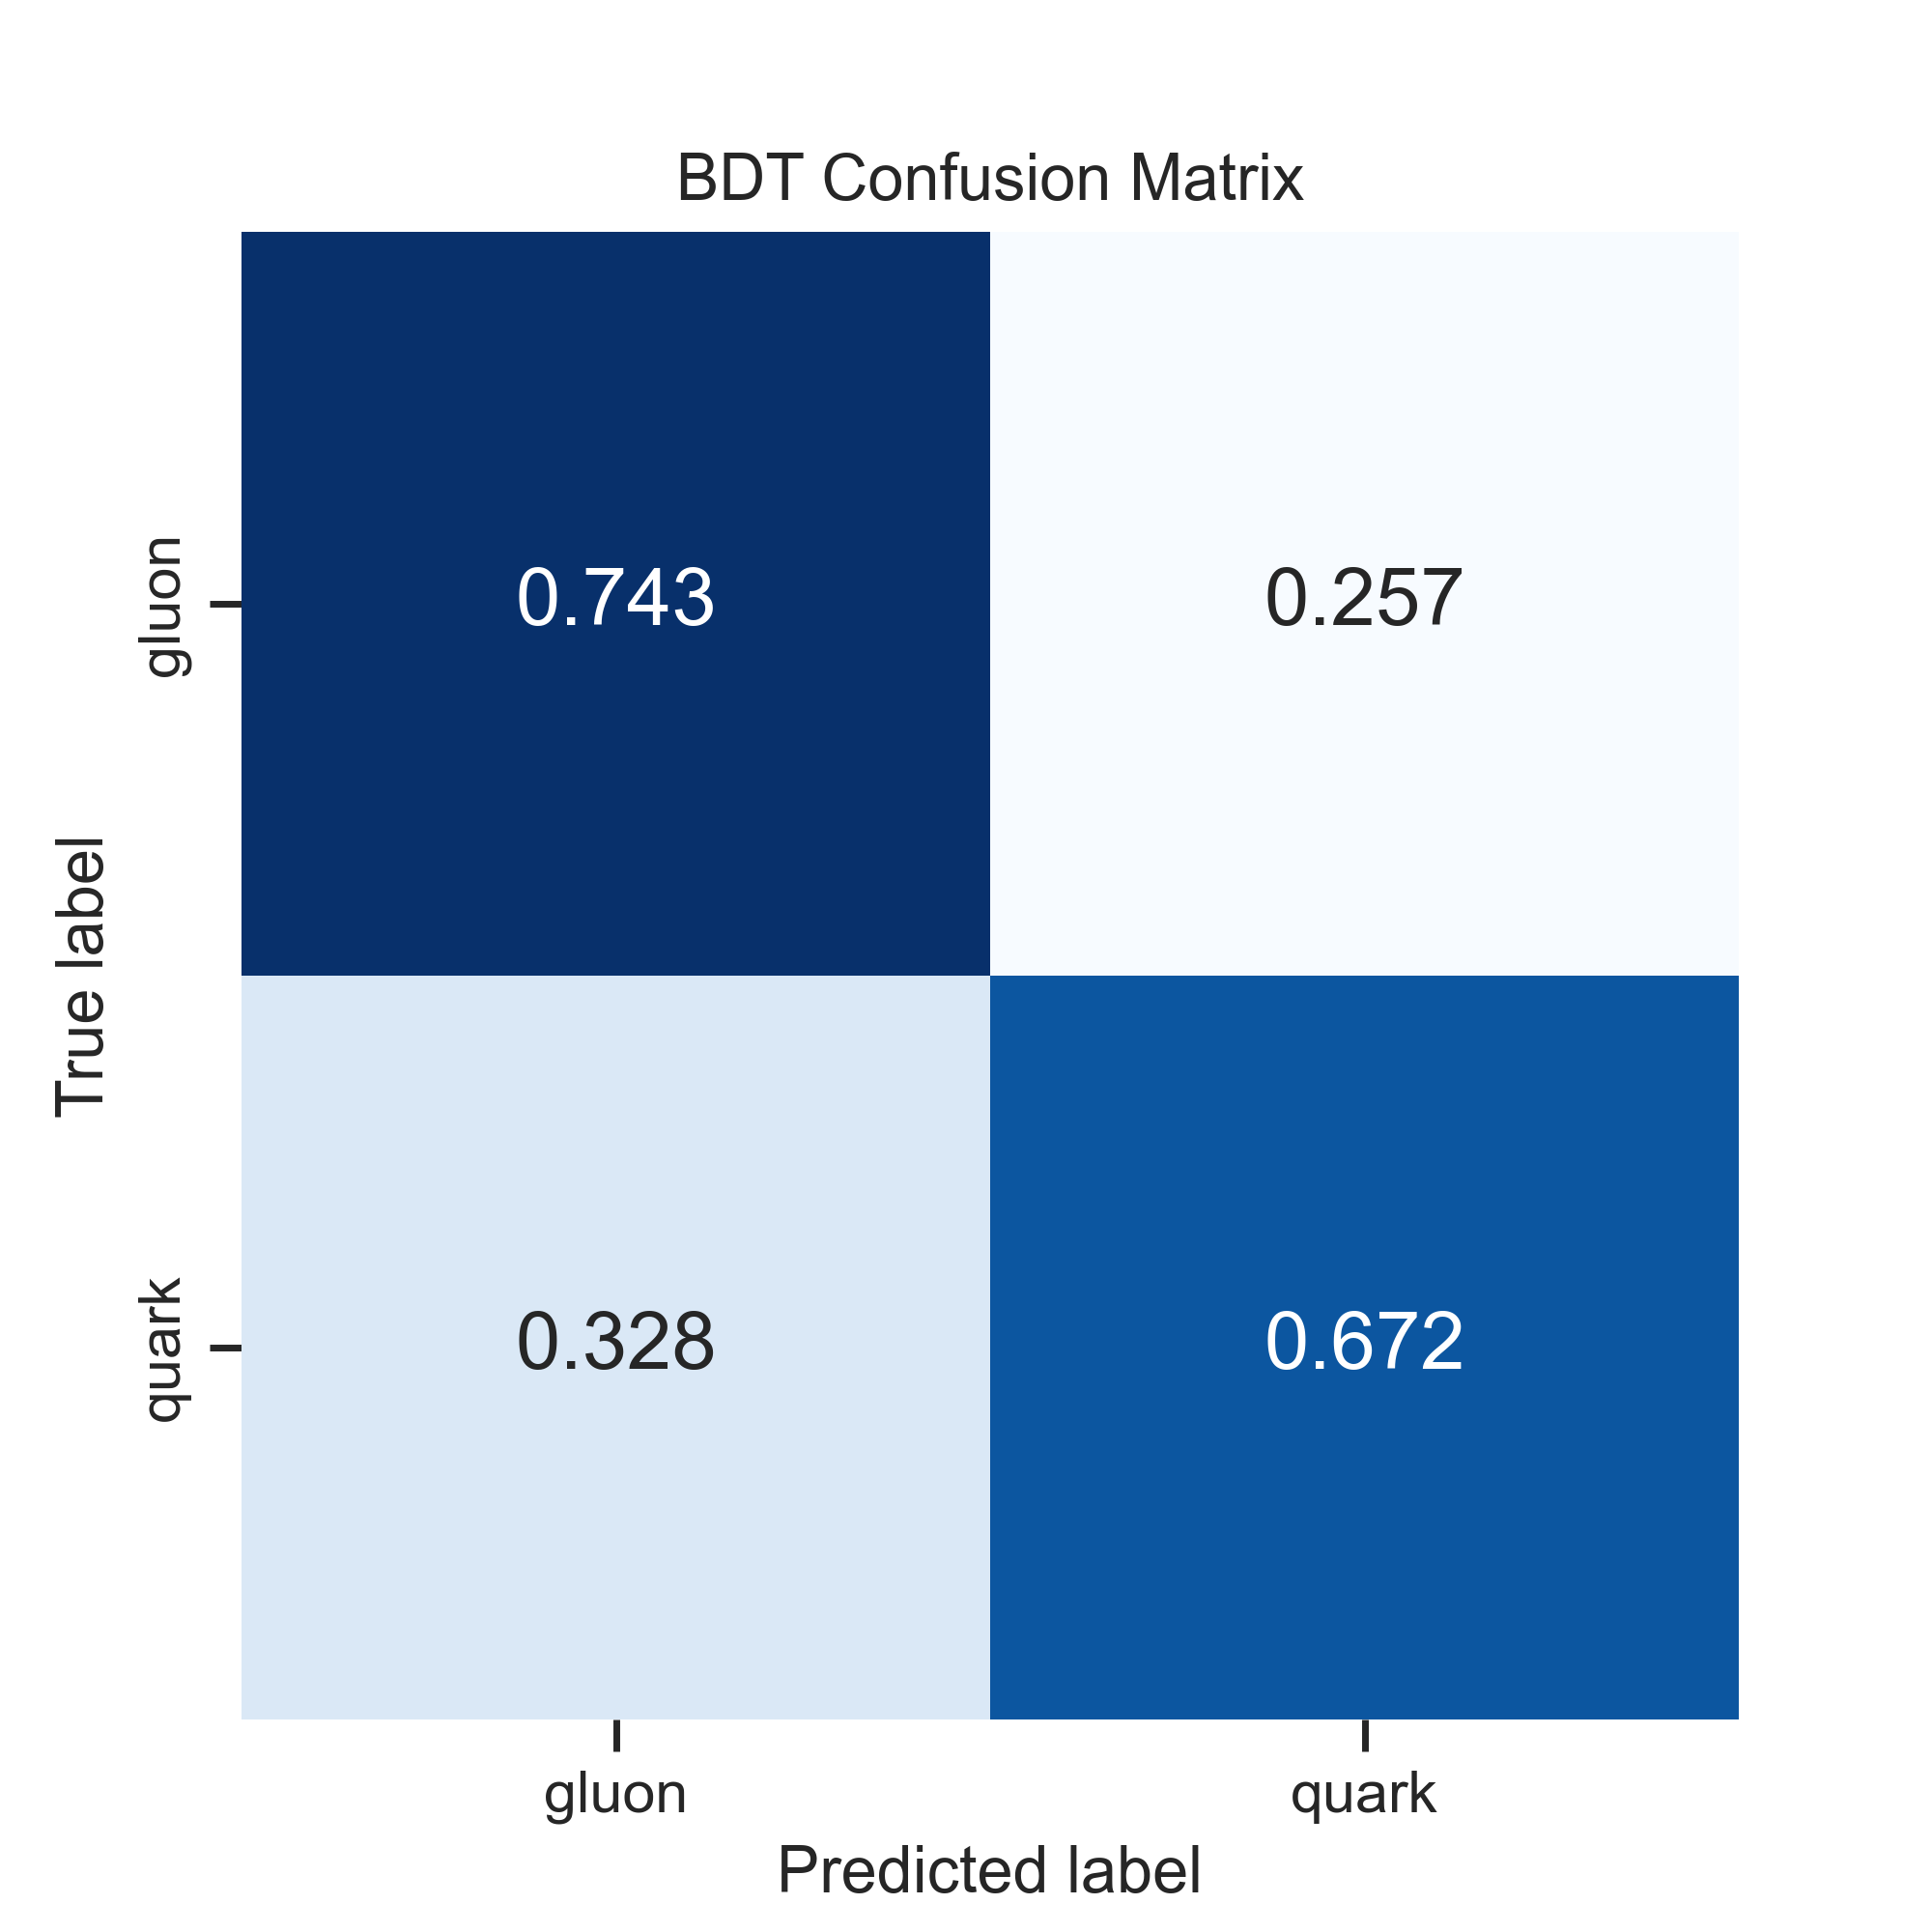
\includegraphics[width=\textwidth]{src/plots/results/cm/bdt.png}
        \caption{BDT}
        \label{fig:confusion_bdt}
    \end{subfigure}
    \caption{Confusion matrices for selected models.}
    \label{fig:confusion}
\end{figure}
\begin{figure}[ht]
    \centering
    \begin{subfigure}[b]{0.49\textwidth}
        \centering
        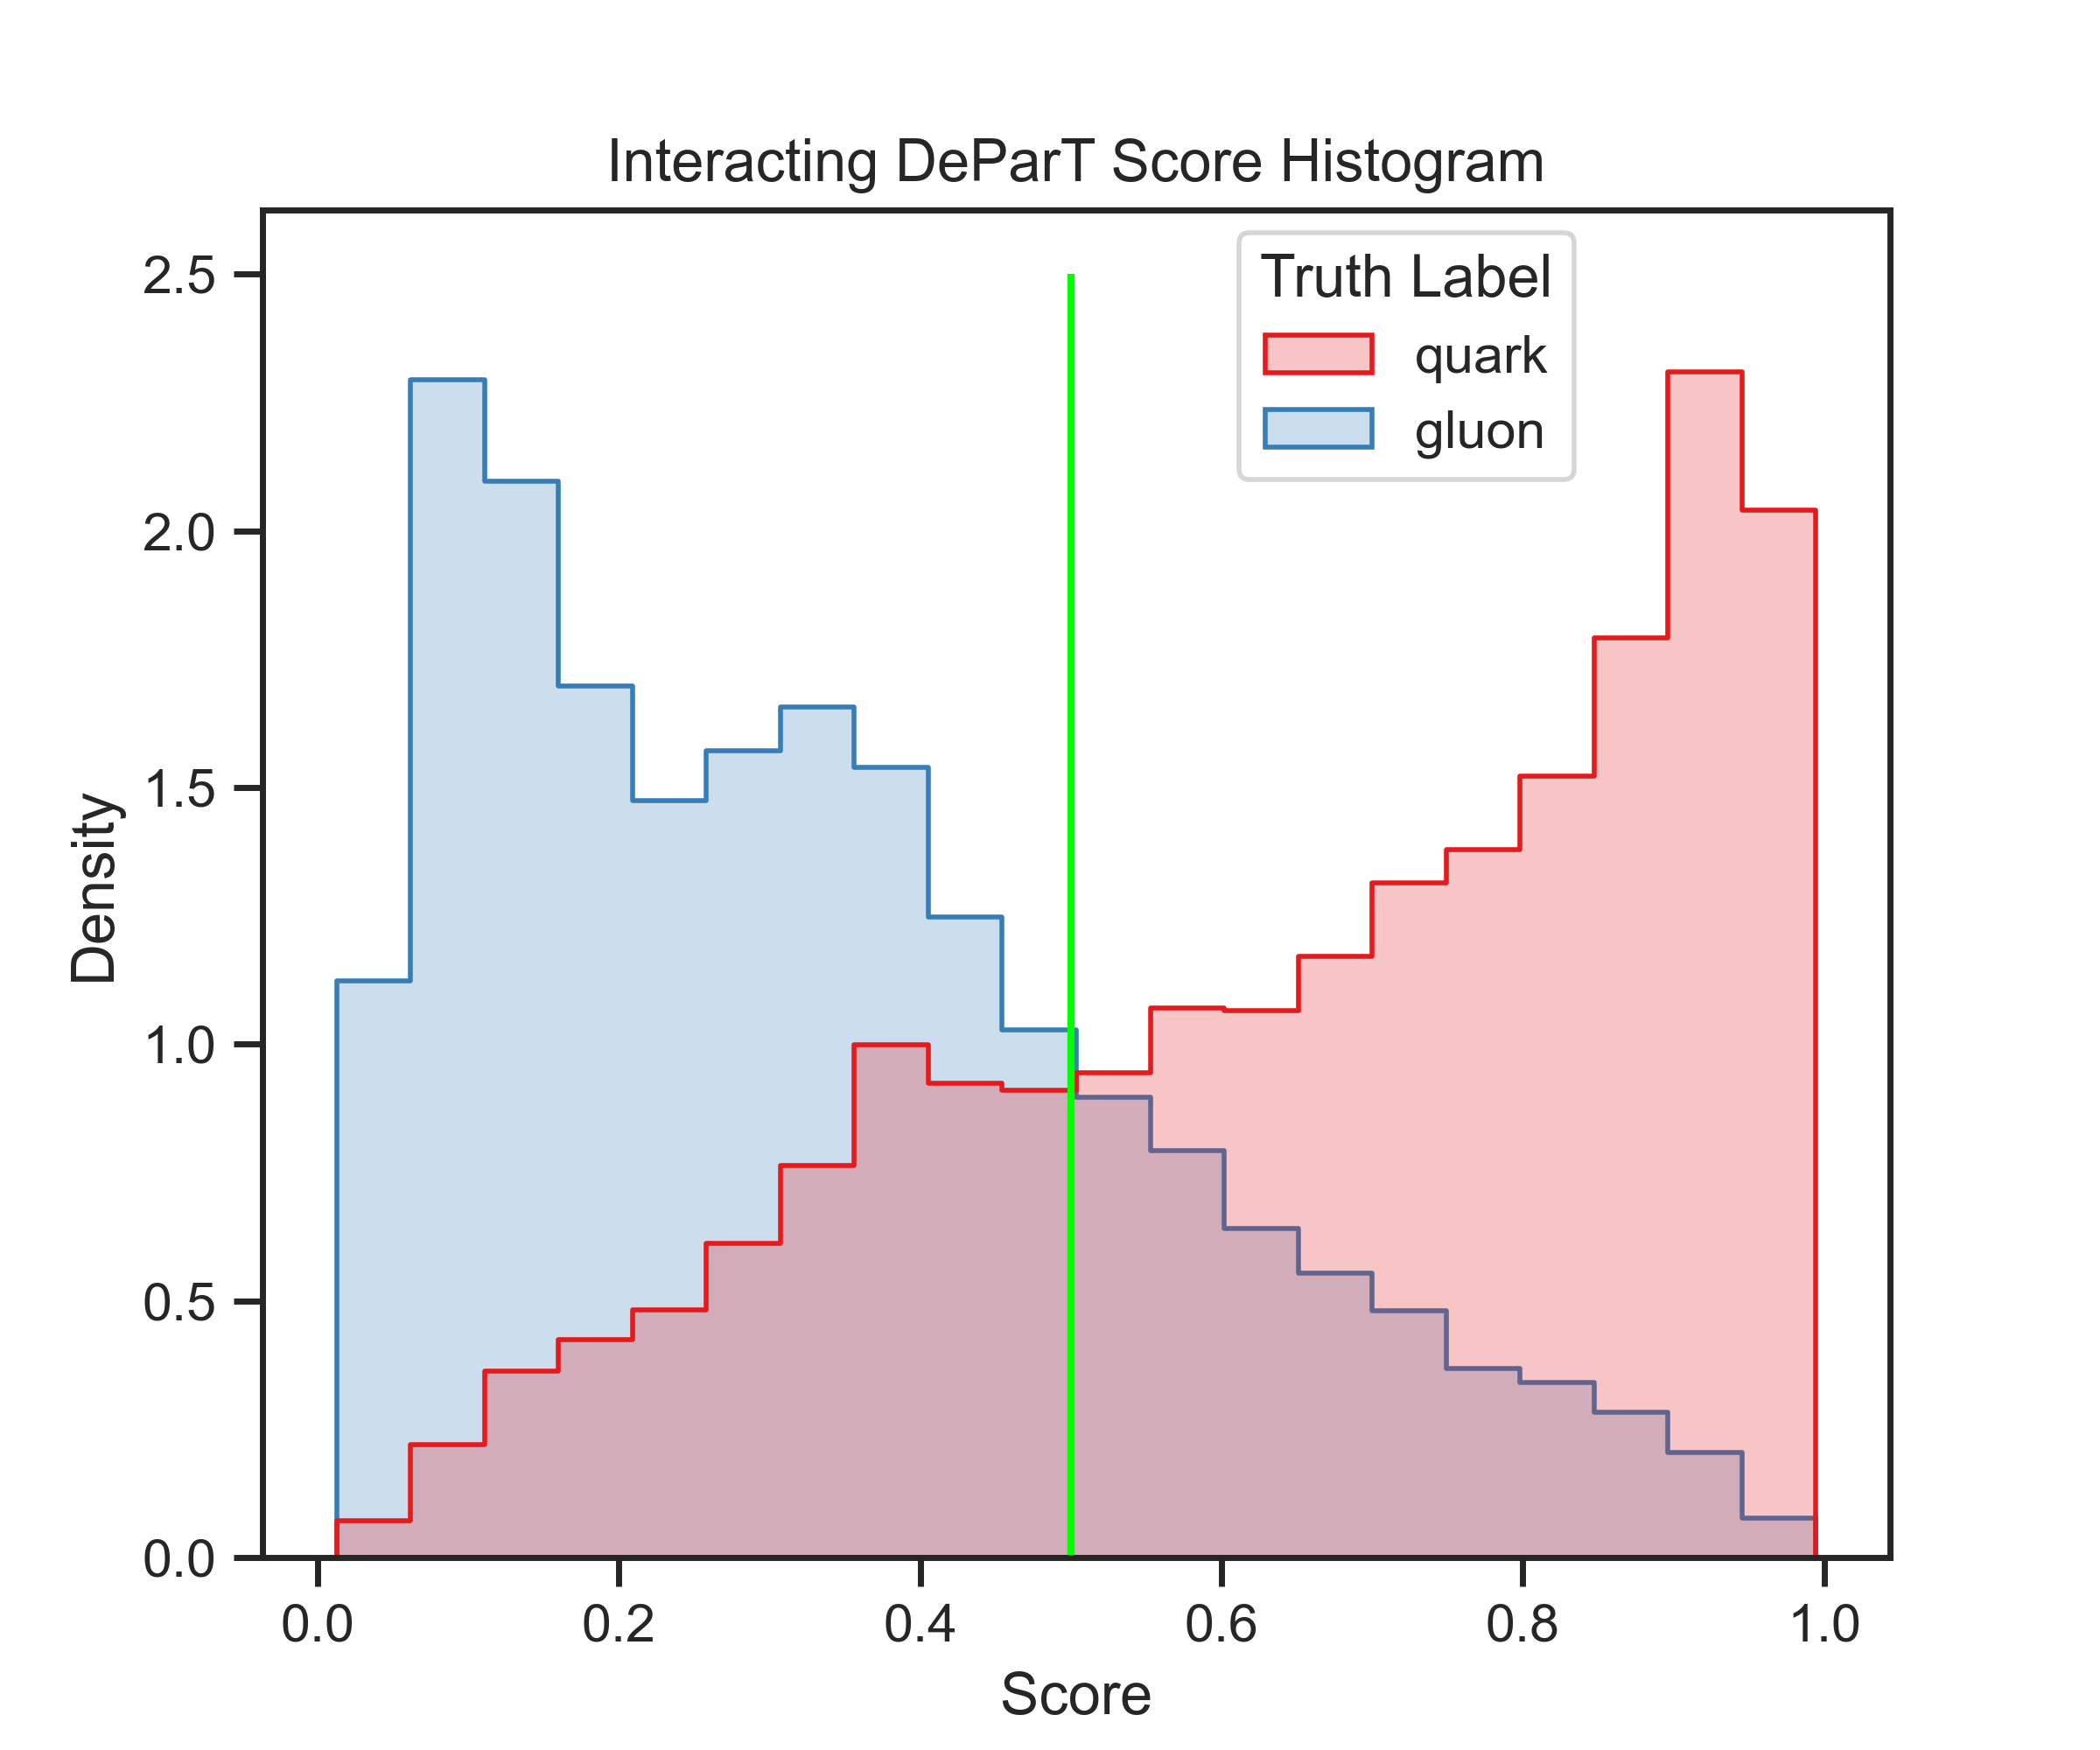
\includegraphics[width=\textwidth]{src/plots/results/score/interacting_depart.png}
        \caption{Interacting DeParT}
        \label{fig:score_depart}
    \end{subfigure}
    % \begin{subfigure}[b]{0.49\textwidth}
    %     \centering
    %     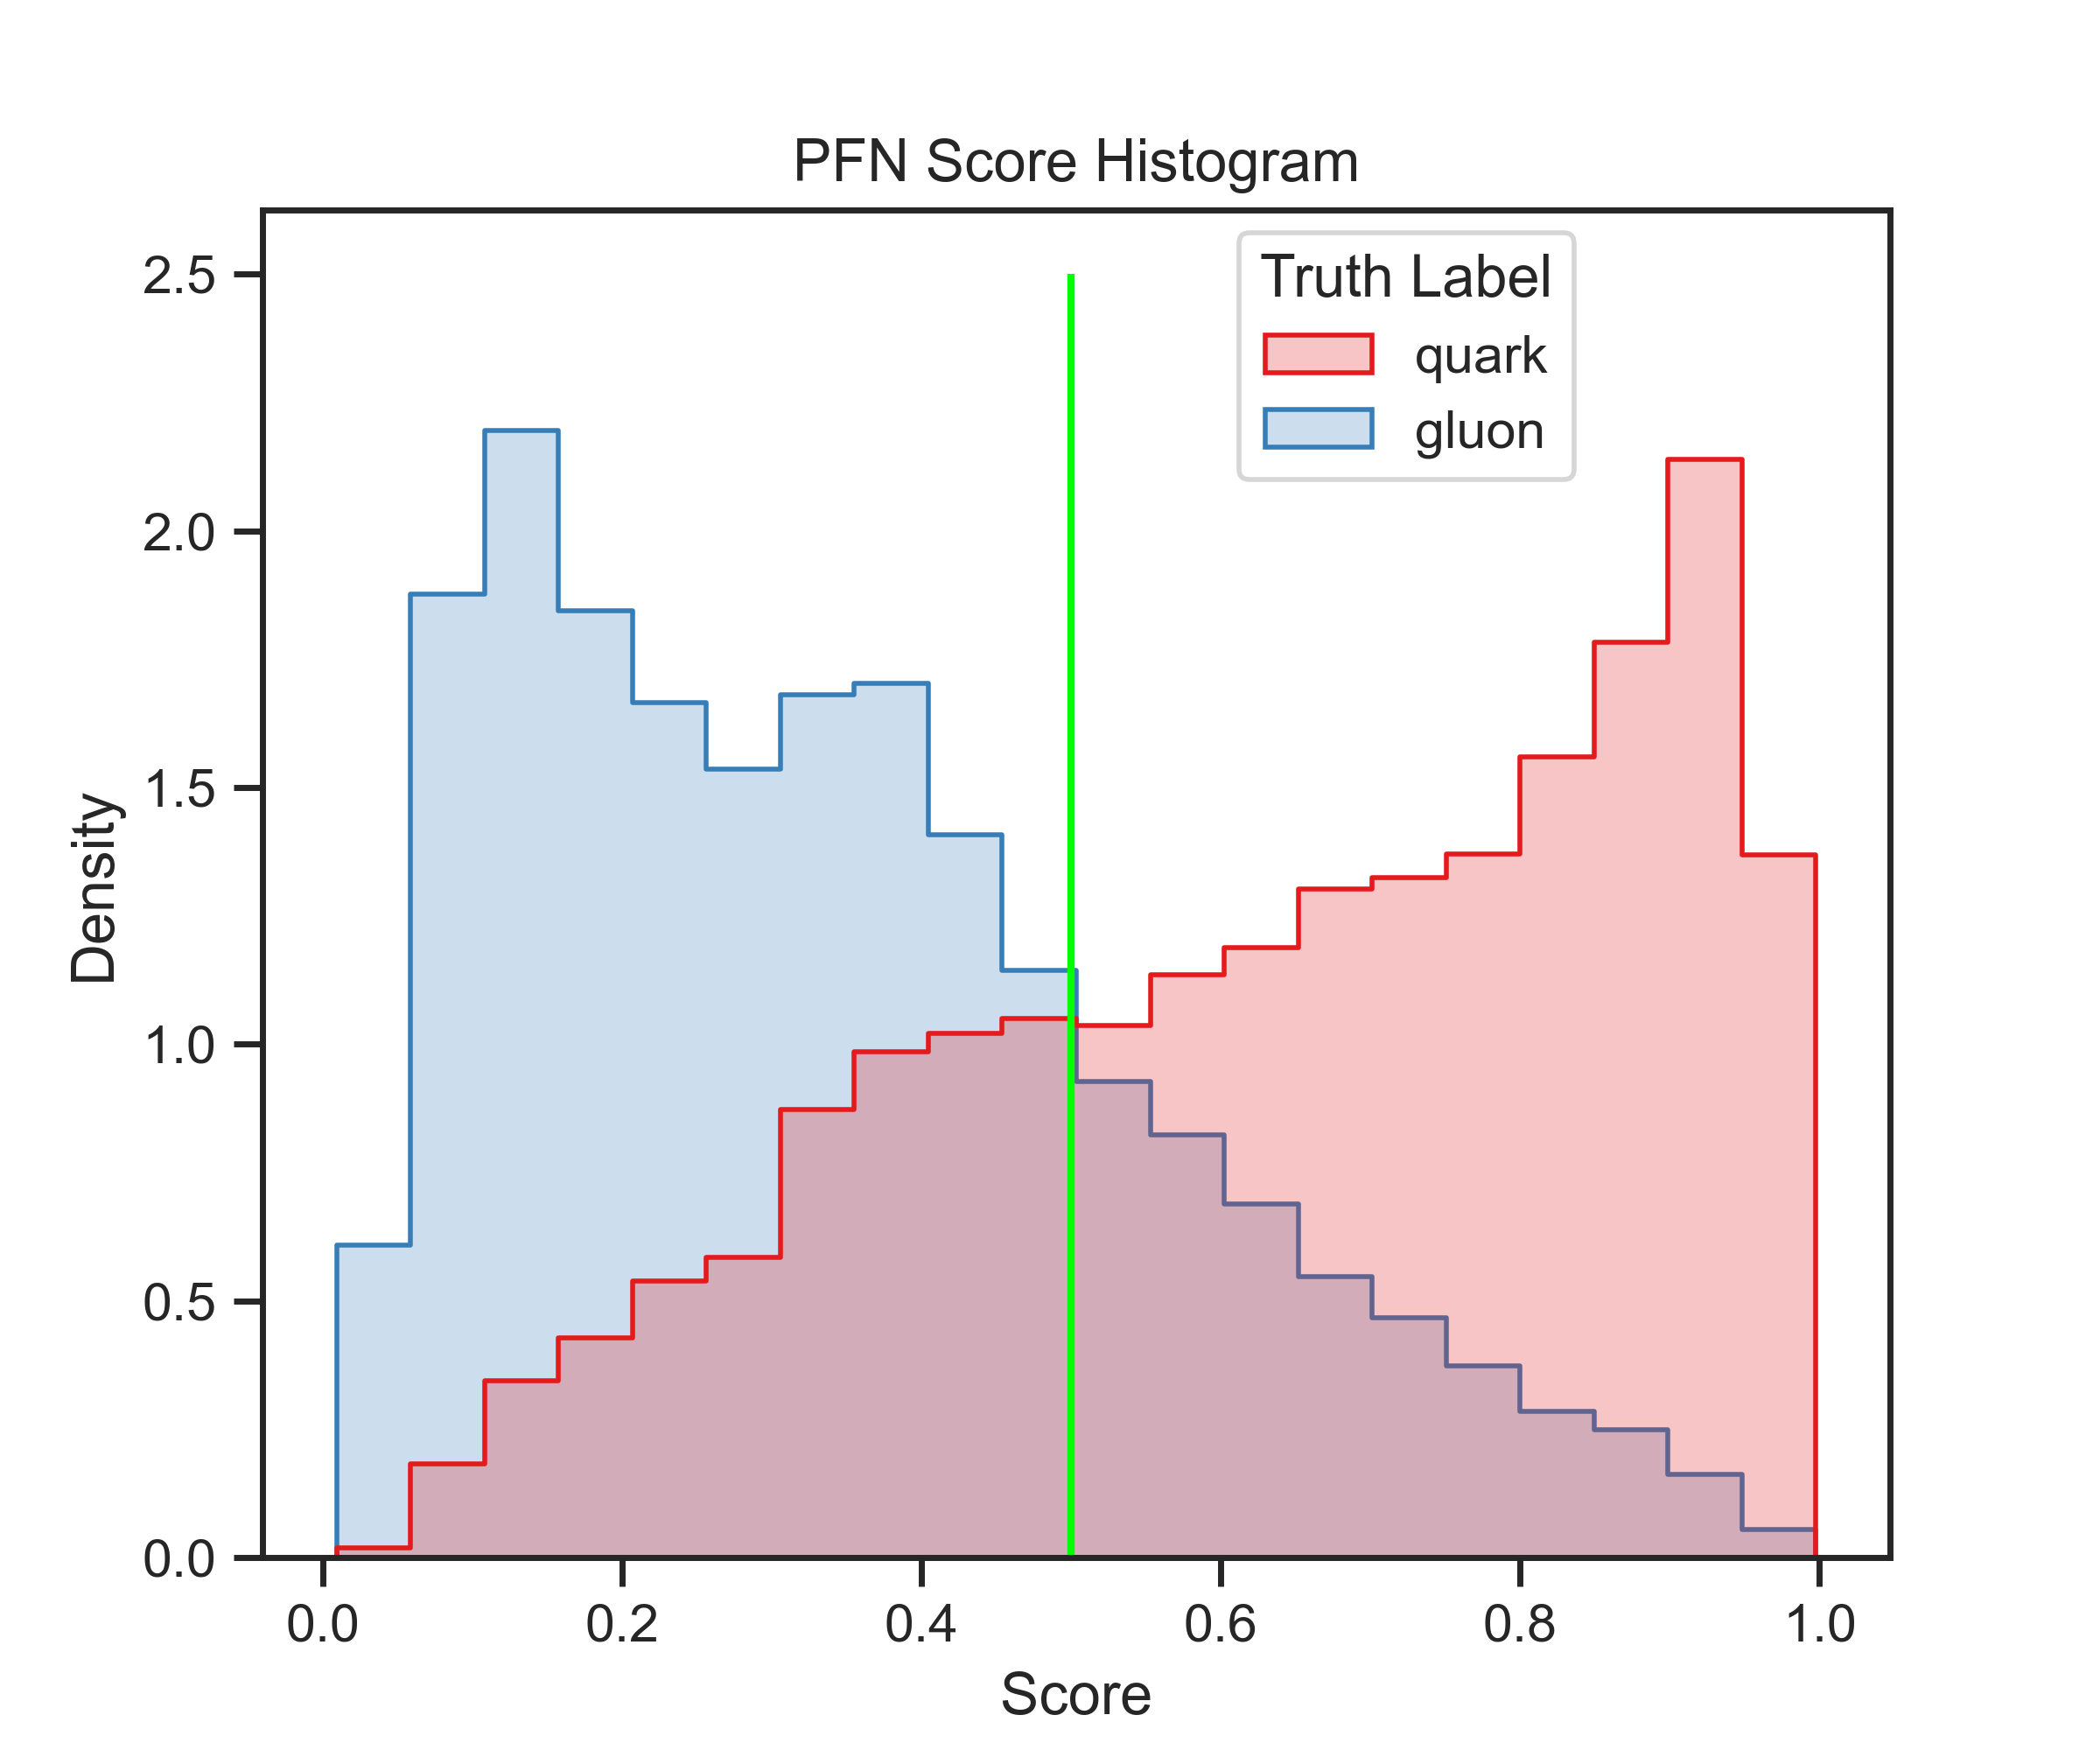
\includegraphics[width=\textwidth]{src/plots/results/score/pfn.png}
    %     \caption{PFN}
    %     \label{fig:score_pfn}
    % \end{subfigure}
    % \begin{subfigure}[b]{0.49\textwidth}
    %     \centering
    %     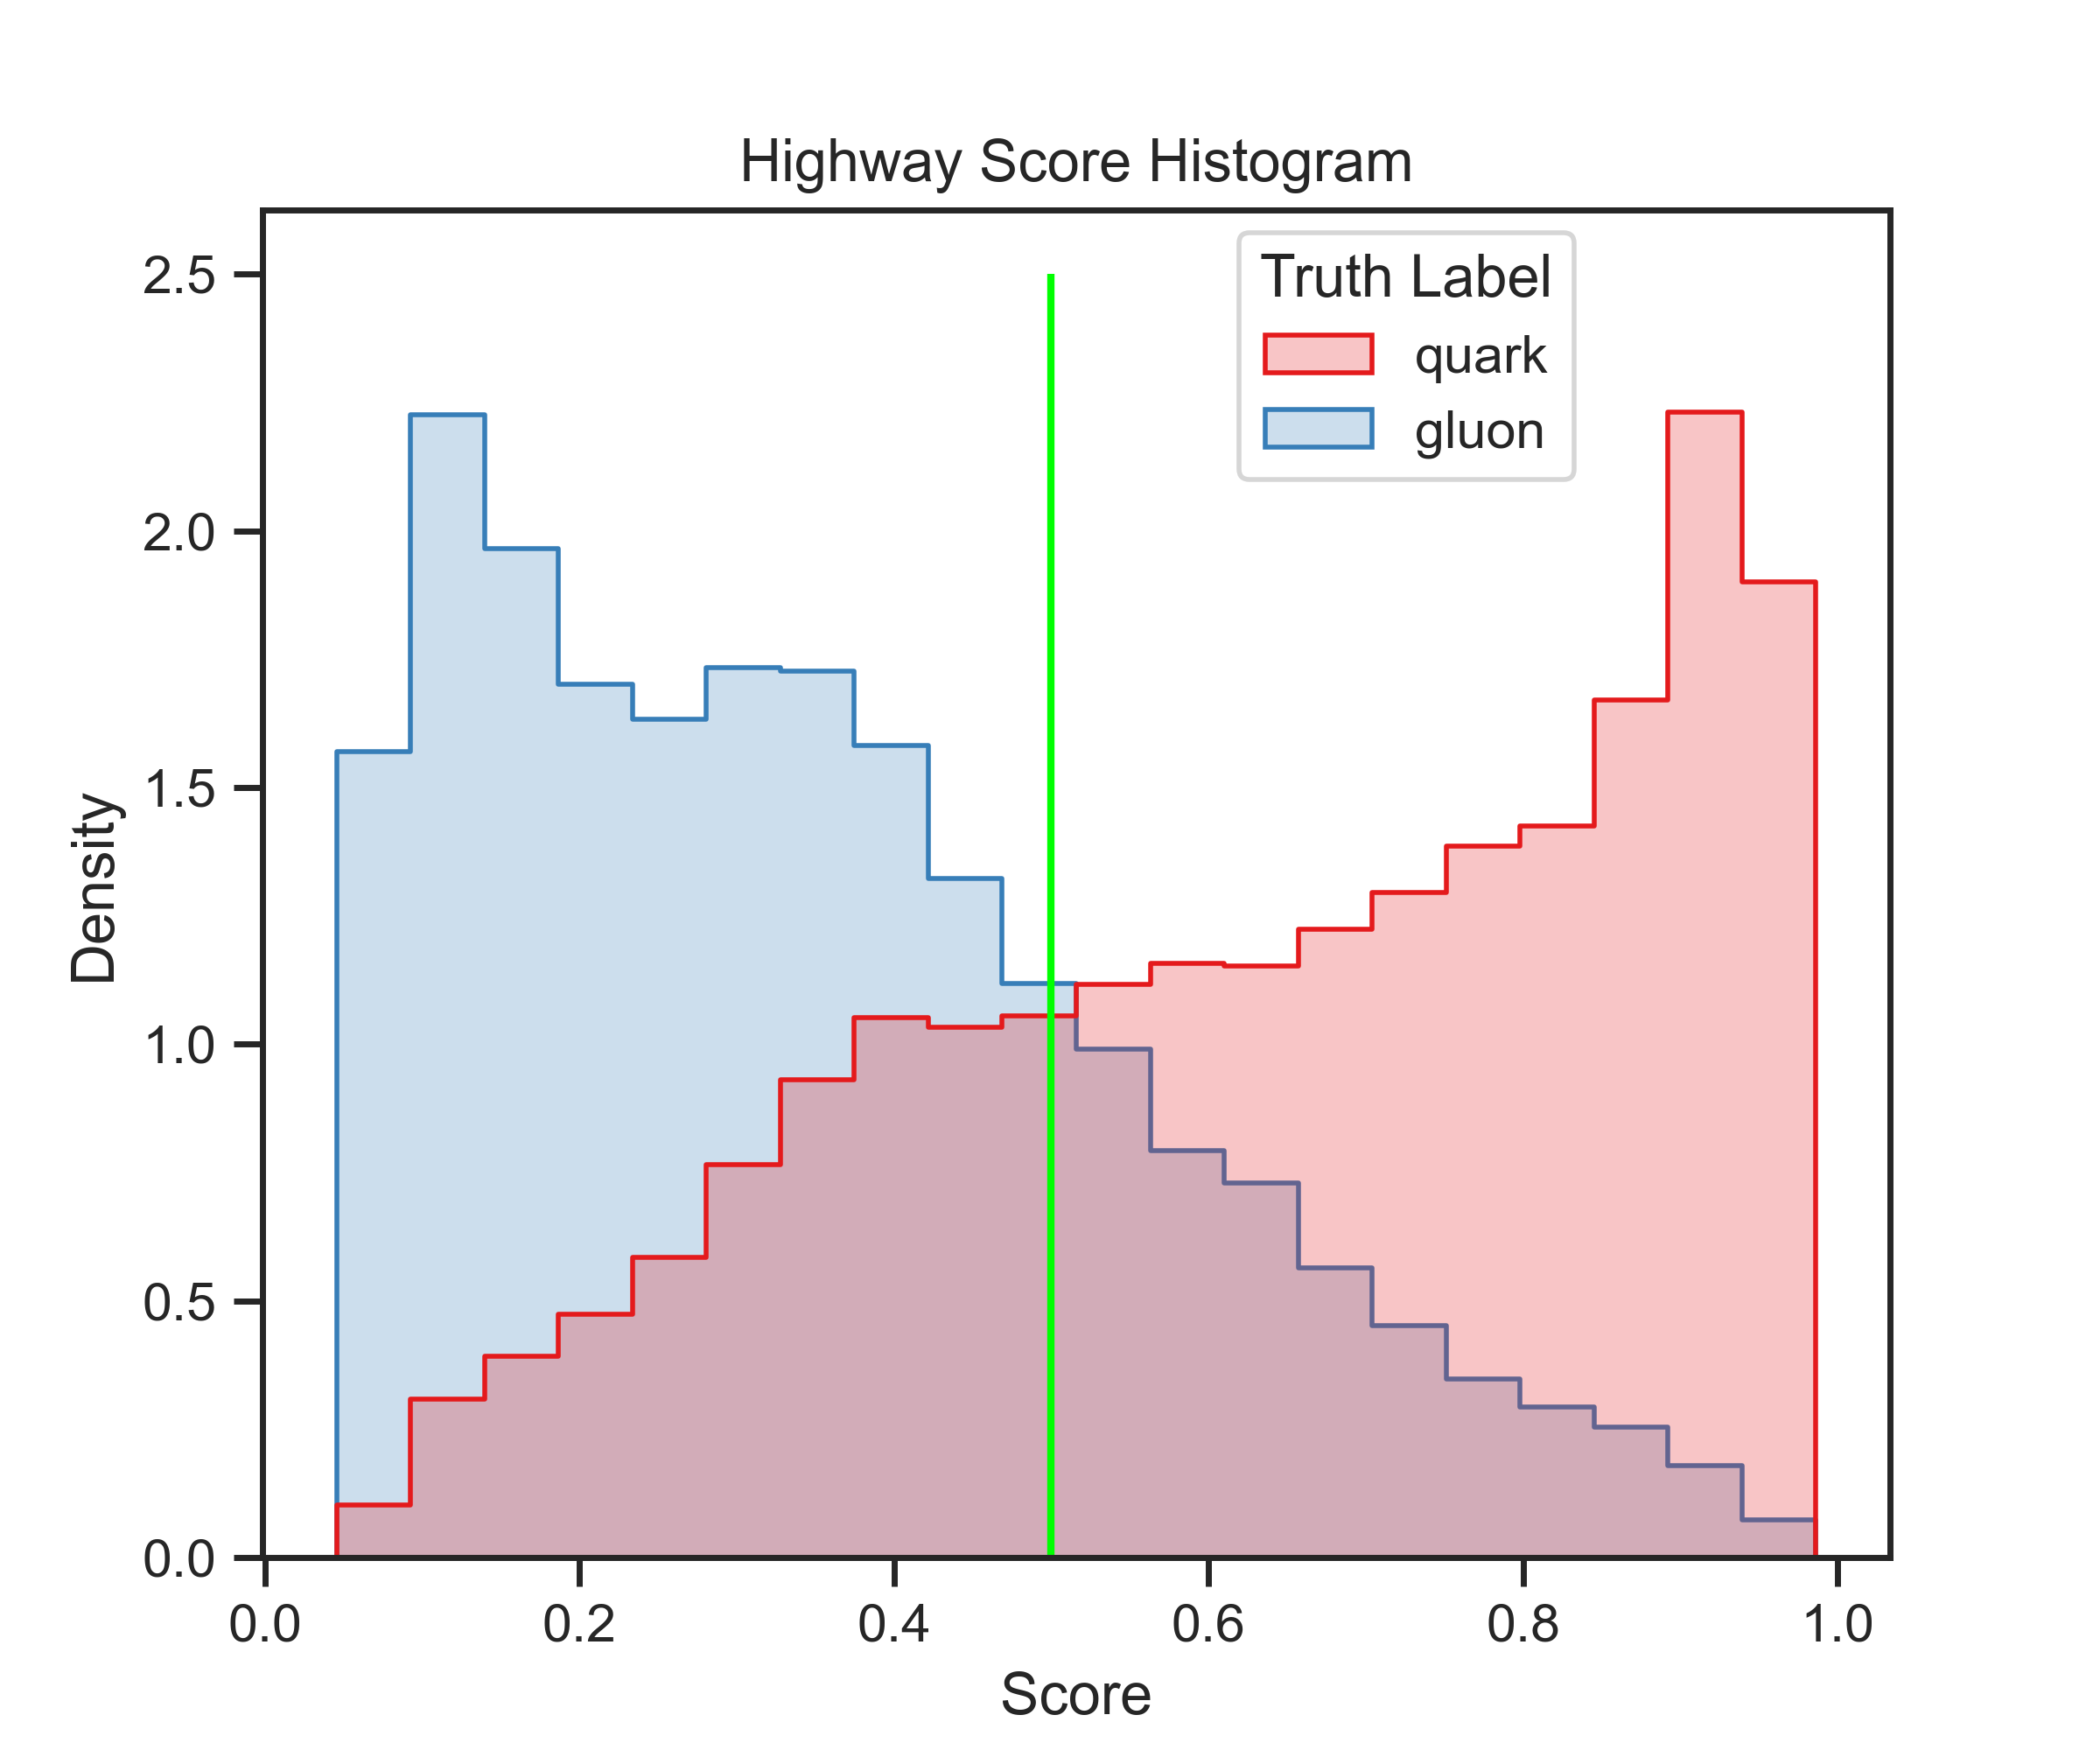
\includegraphics[width=\textwidth]{src/plots/results/score/highway.png}
    %     \caption{Highway}
    %     \label{fig:score_depart_inter}
    % \end{subfigure}
    \begin{subfigure}[b]{0.49\textwidth}
        \centering
        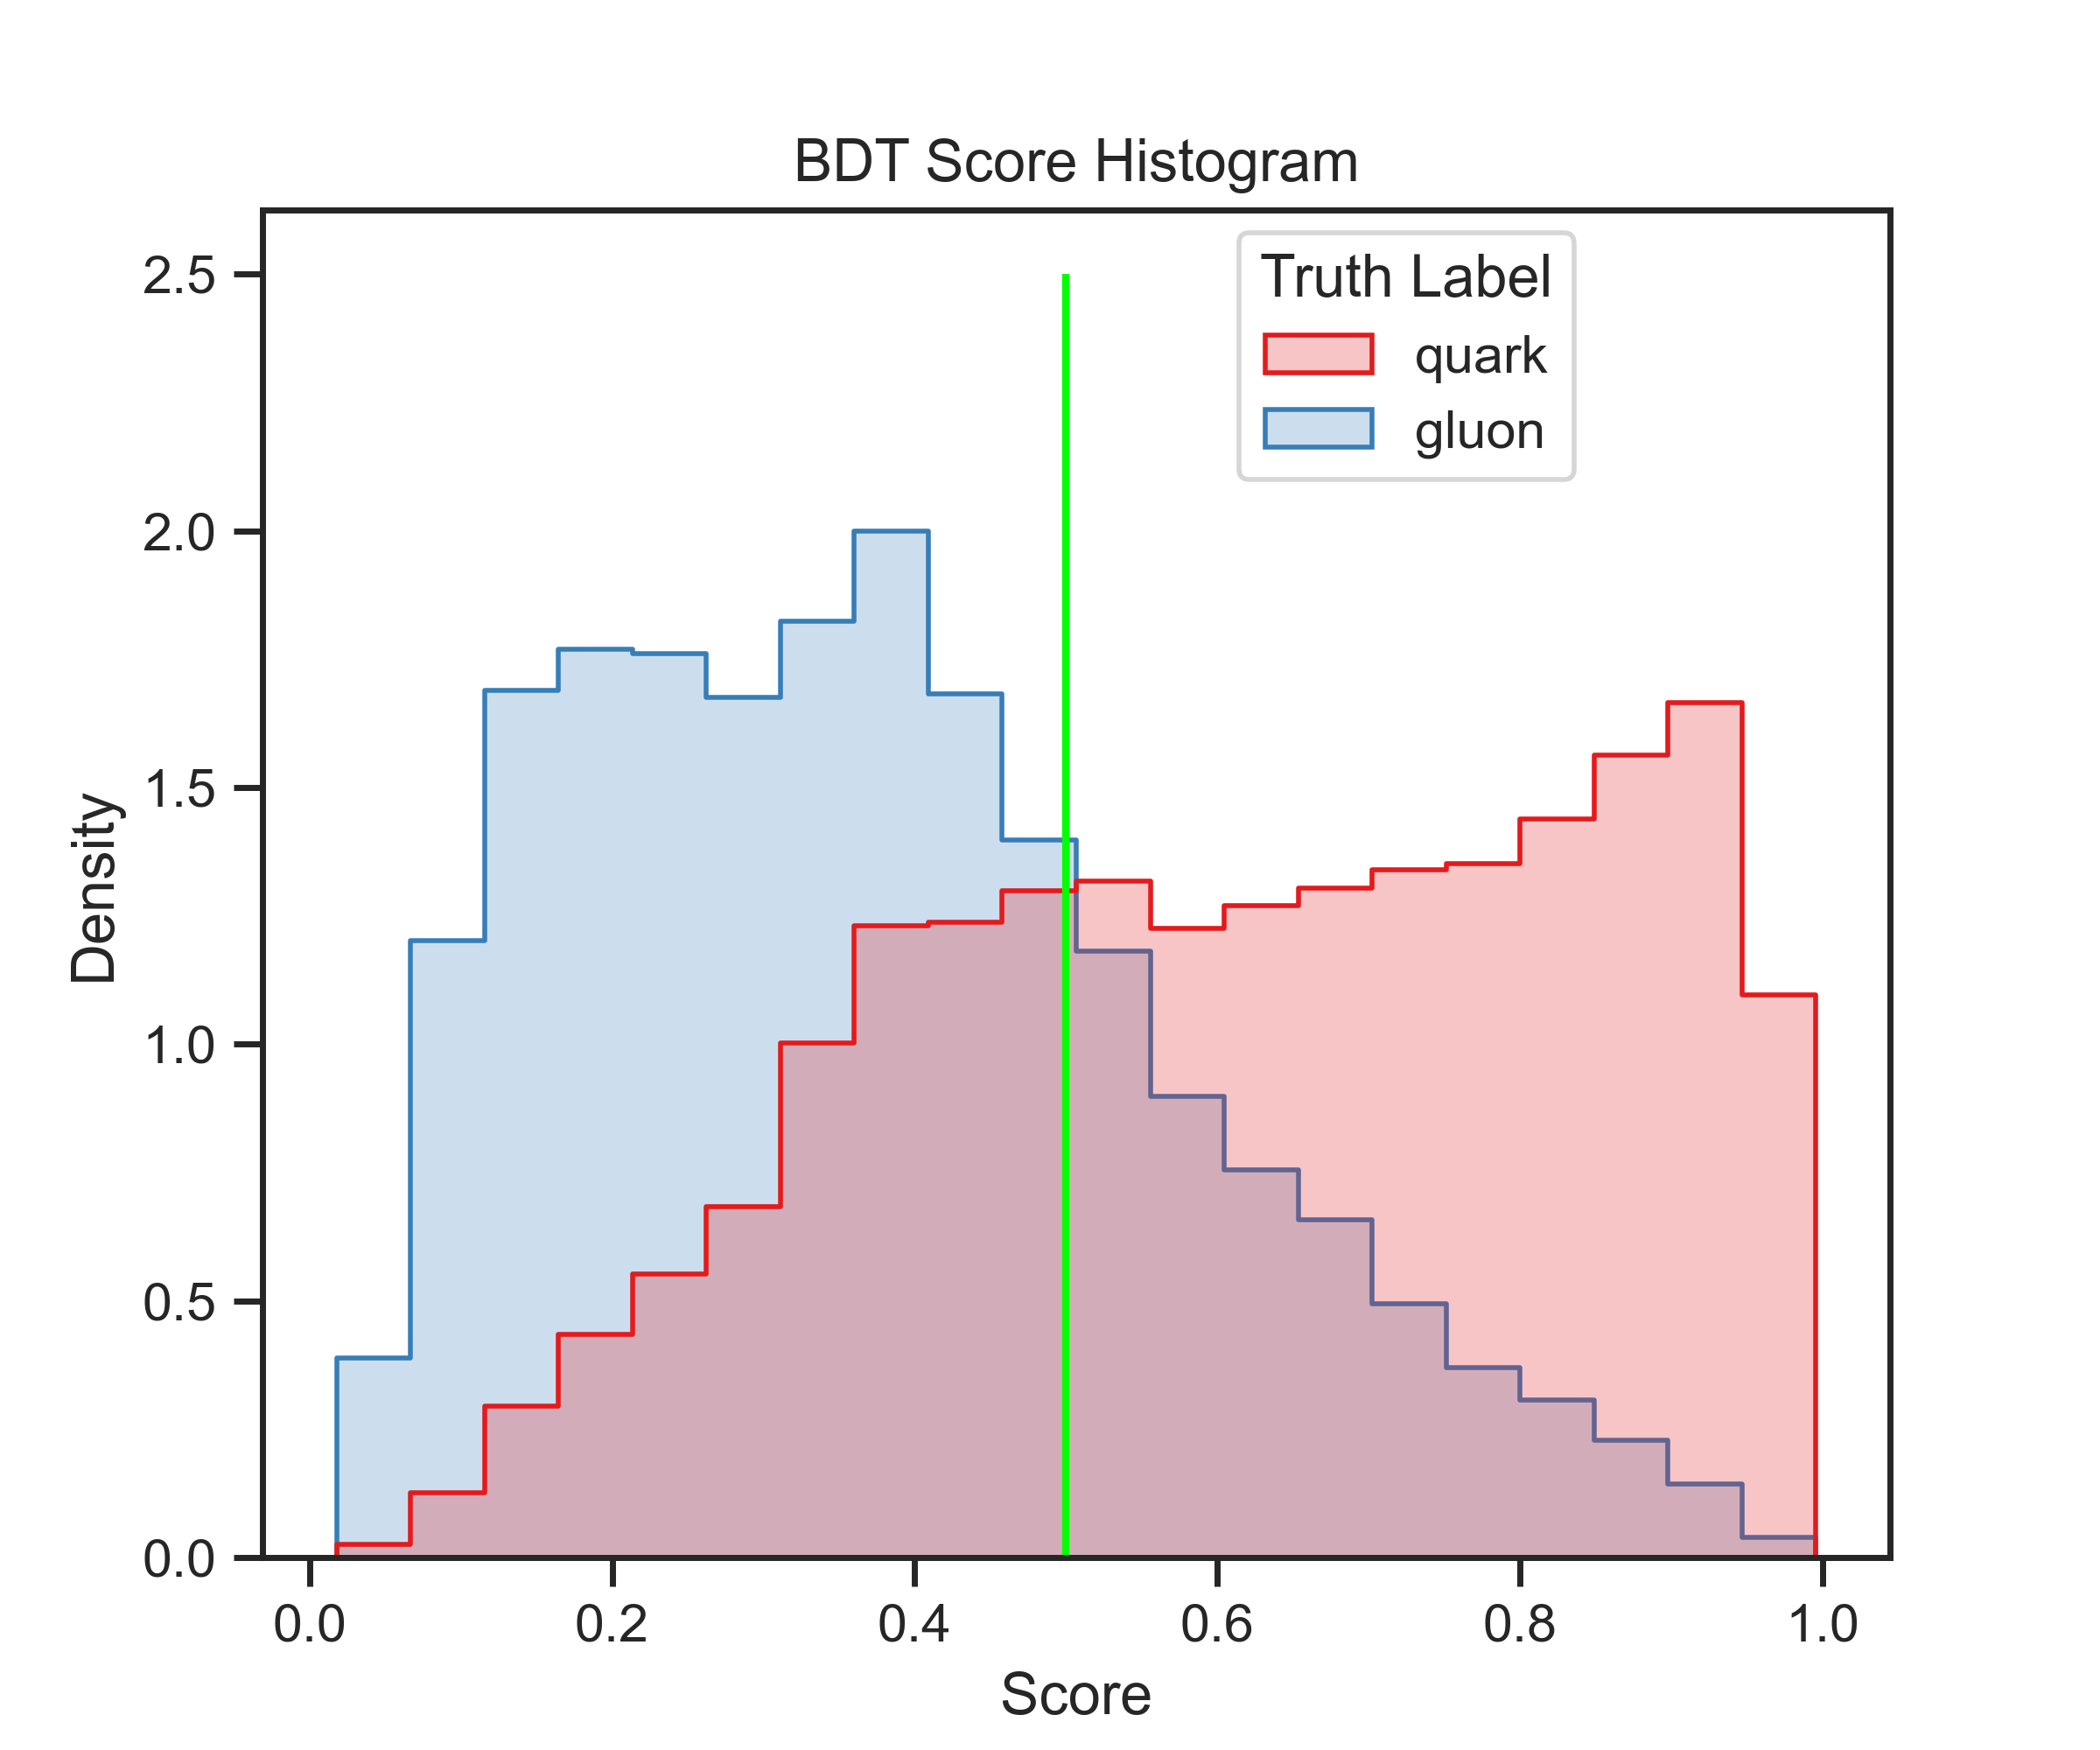
\includegraphics[width=\textwidth]{src/plots/results/score/bdt.png}
        \caption{BDT}
        \label{fig:score_bdt}
    \end{subfigure}
    \caption{Output scores for selected models colored by the Truth Label. The lime line represents the classification threshold; everything left is tagged as a gluon, and everything right is tagged as a quark.}
    \label{fig:score}
\end{figure}

Even though the interaction variables are computed from the \PFO variables, i.e., the model can learn how to calculate them without being explicitly told, and they still improve the performance.
Because every head is given different input, it helps them focus on various aspects of the jet, and when combined, they can learn more complex patterns.
Even more, allowing the heads to talk to each other (something that \ParT has not, but \depart does) improves the performance.
On the other hand, interaction variables make the computation more expensive because they are used as a second input, the memory usage is much higher, and the inference time is longer, as seen in \cref{tab:tech}.


Another exciting aspect is the inference time of the models, \bdt especially. 
Since \bdt dost not run on the GPU, it is significantly slower than \highway and \fc, which are far more complex models.
On top of that, even \EFN and \PFN that use \PFO variables are faster than \bdt.

Confusion Matrices are shown in \cref{fig:confusion} for selected models (the rest is in \cref{sec:app_confusion}).
They follow a similar pattern, where the quarks are more challenging to distinguish from the gluons than the gluons from the quarks.
This can be seen from the lower left corner, where the quarks are misclassified as gluons.

Score outputs colored by their Truth Label of the selected models are shown in \cref{fig:score} (the rest is in \cref{sec:app_scorehist}).
The middle lime line, at 0.5, is the threshold for the classification, everything left is classified as a gluon, and everything right is classified as a quark.
The \depart model on \cref{fig:score_depart} has better separation between the two classes than the \bdt.
However, all models have a small peak at 0.4, where they all suffer from misclassification.
This peak comes from low $\pT$ jets, where the tagging is limited, as discussed in \cref{sec:pt_dependance}.

We have demonstrated the unsatisfactory performance of the previously used model, \bdt, and the superiority of our proposed model, \depart.
In the following sections, we will look at the dependence of the performance on the $\pT$, $\eta$, and the pileup $\mu$.
We will omit the \bdt model from the plots, as it is irrelevant and makes the plots unreadable.

\subsection{Transverse Momentum Dependence}
\label{sec:pt_dependance}
\begin{figure}[htb]
    \centering
    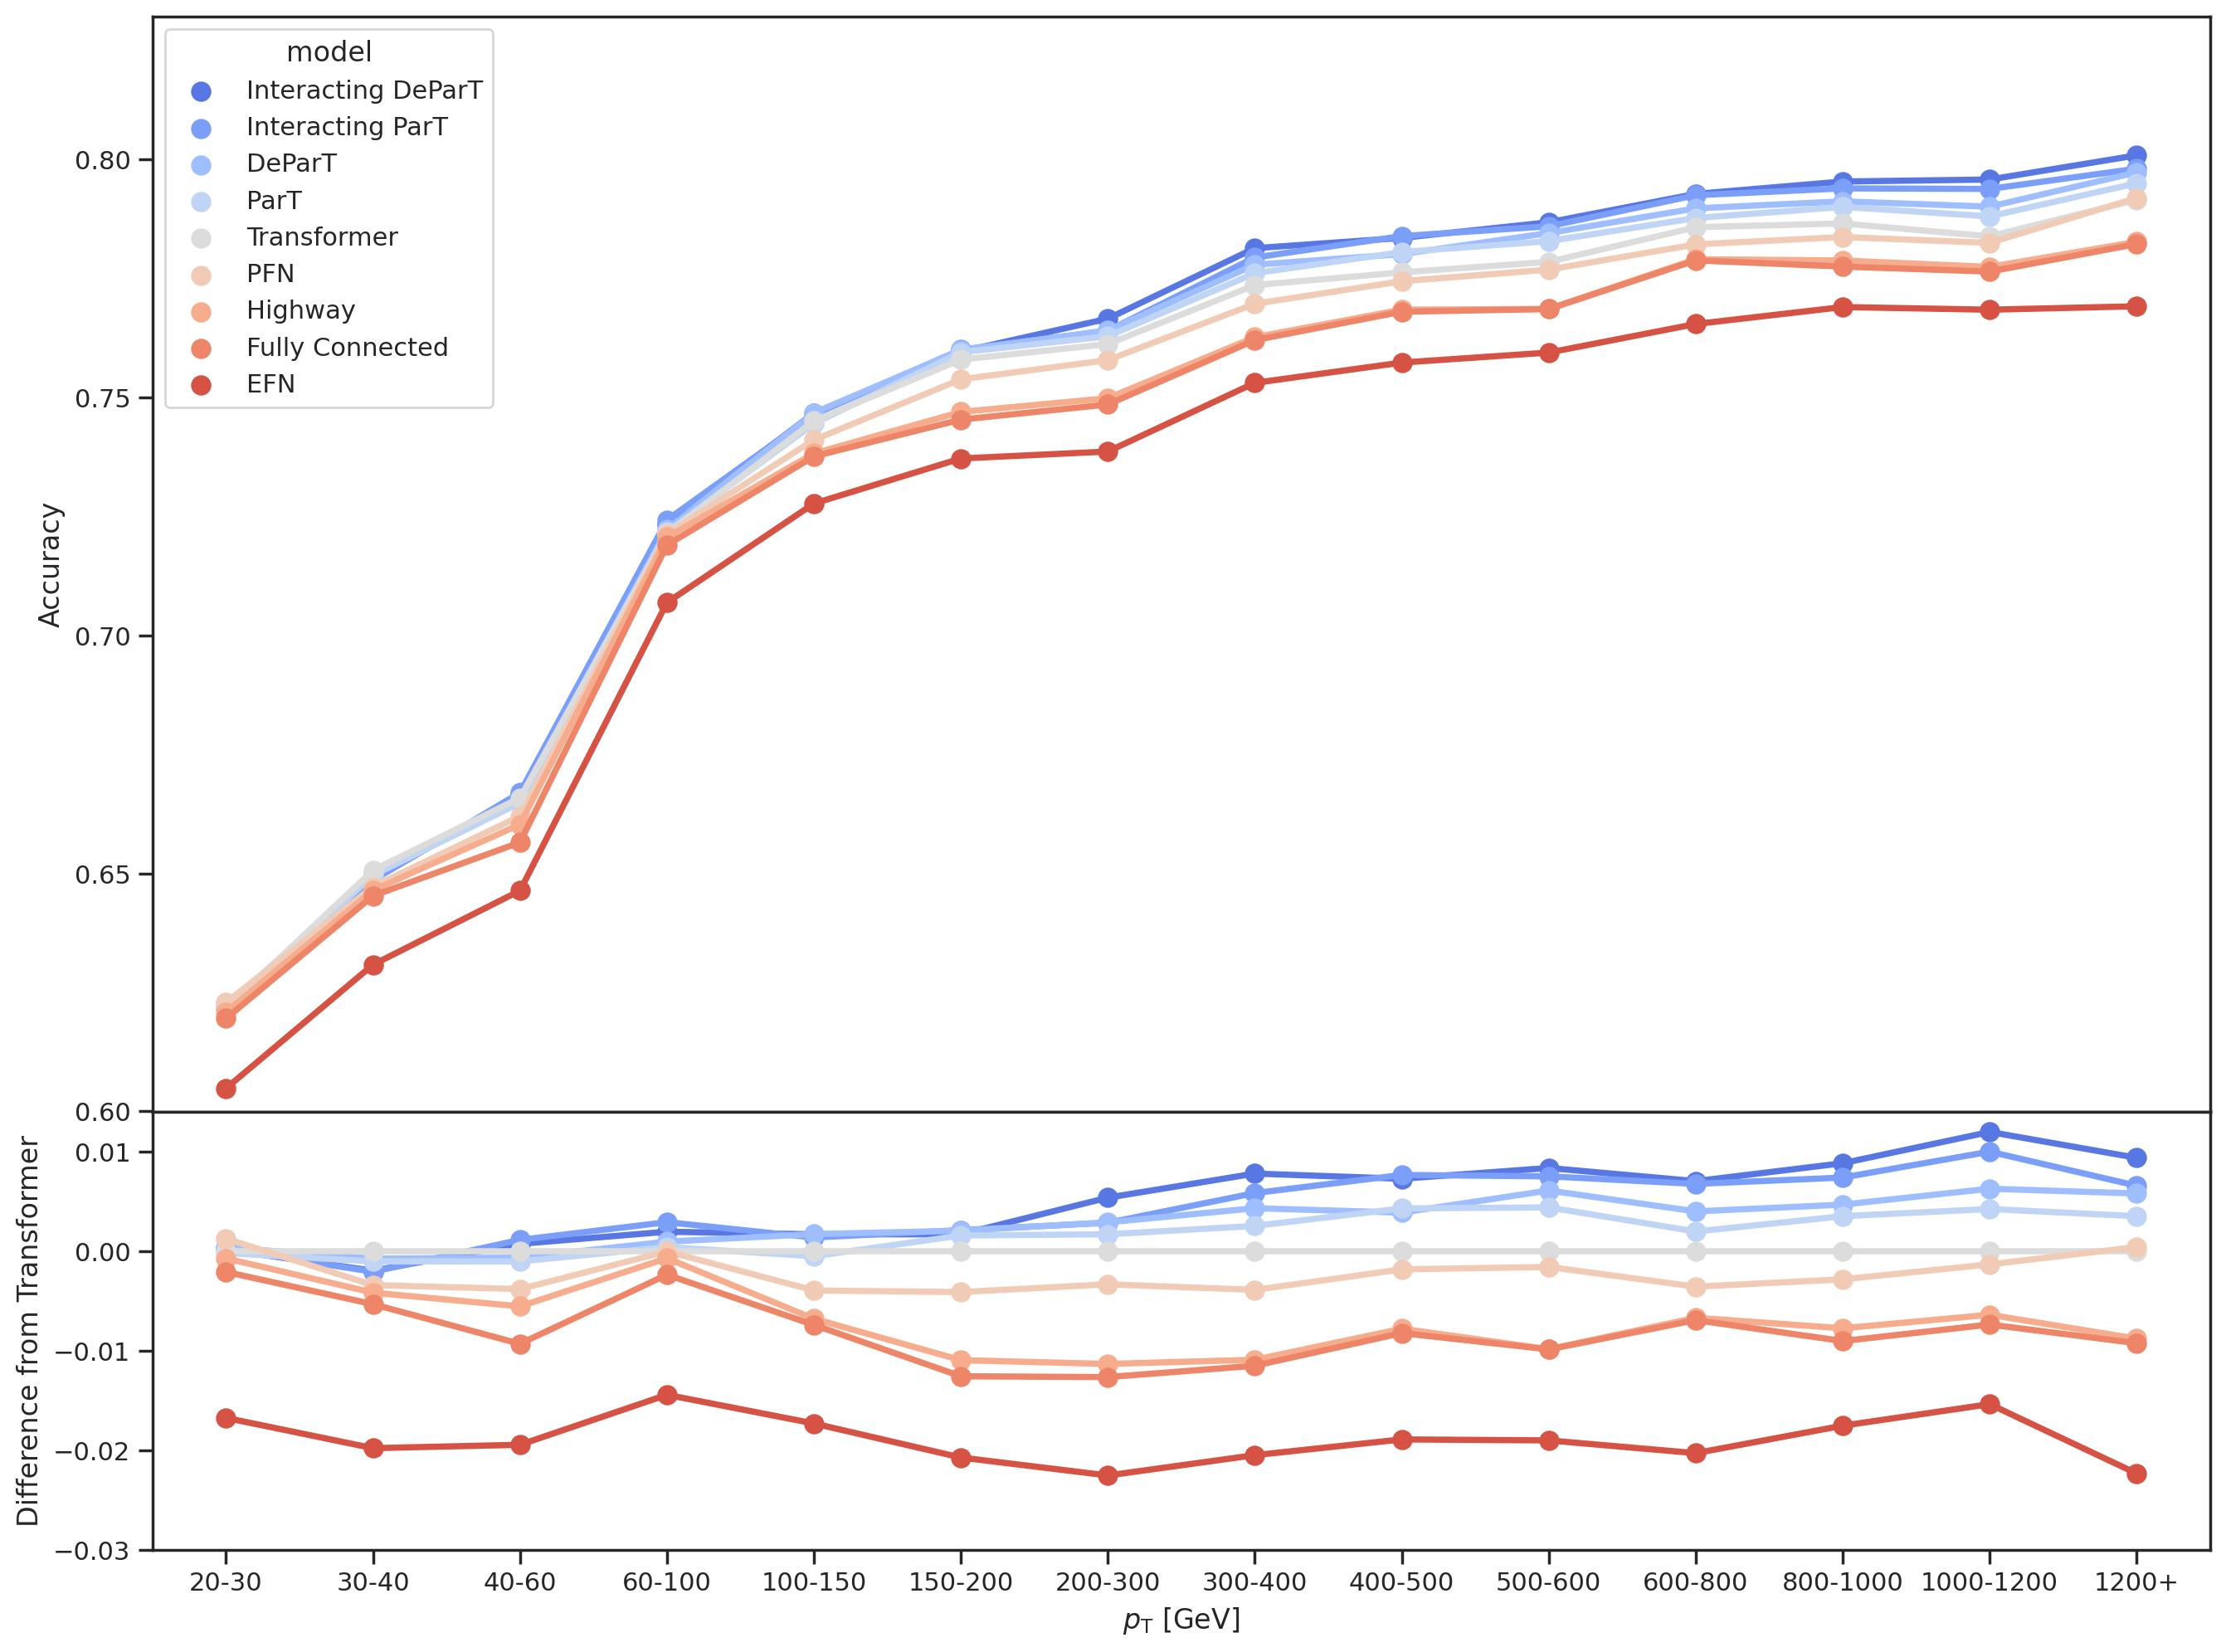
\includegraphics[width=1\linewidth]{src/plots/results/pT_dep/relative_accuracy.jpg}
    \caption{Accuracy of the models as a function of $\pT$ and relative to the Transformer model.}
    \label{fig:pt_dep_acc}
\end{figure}
\begin{figure}[htb]
    \centering
    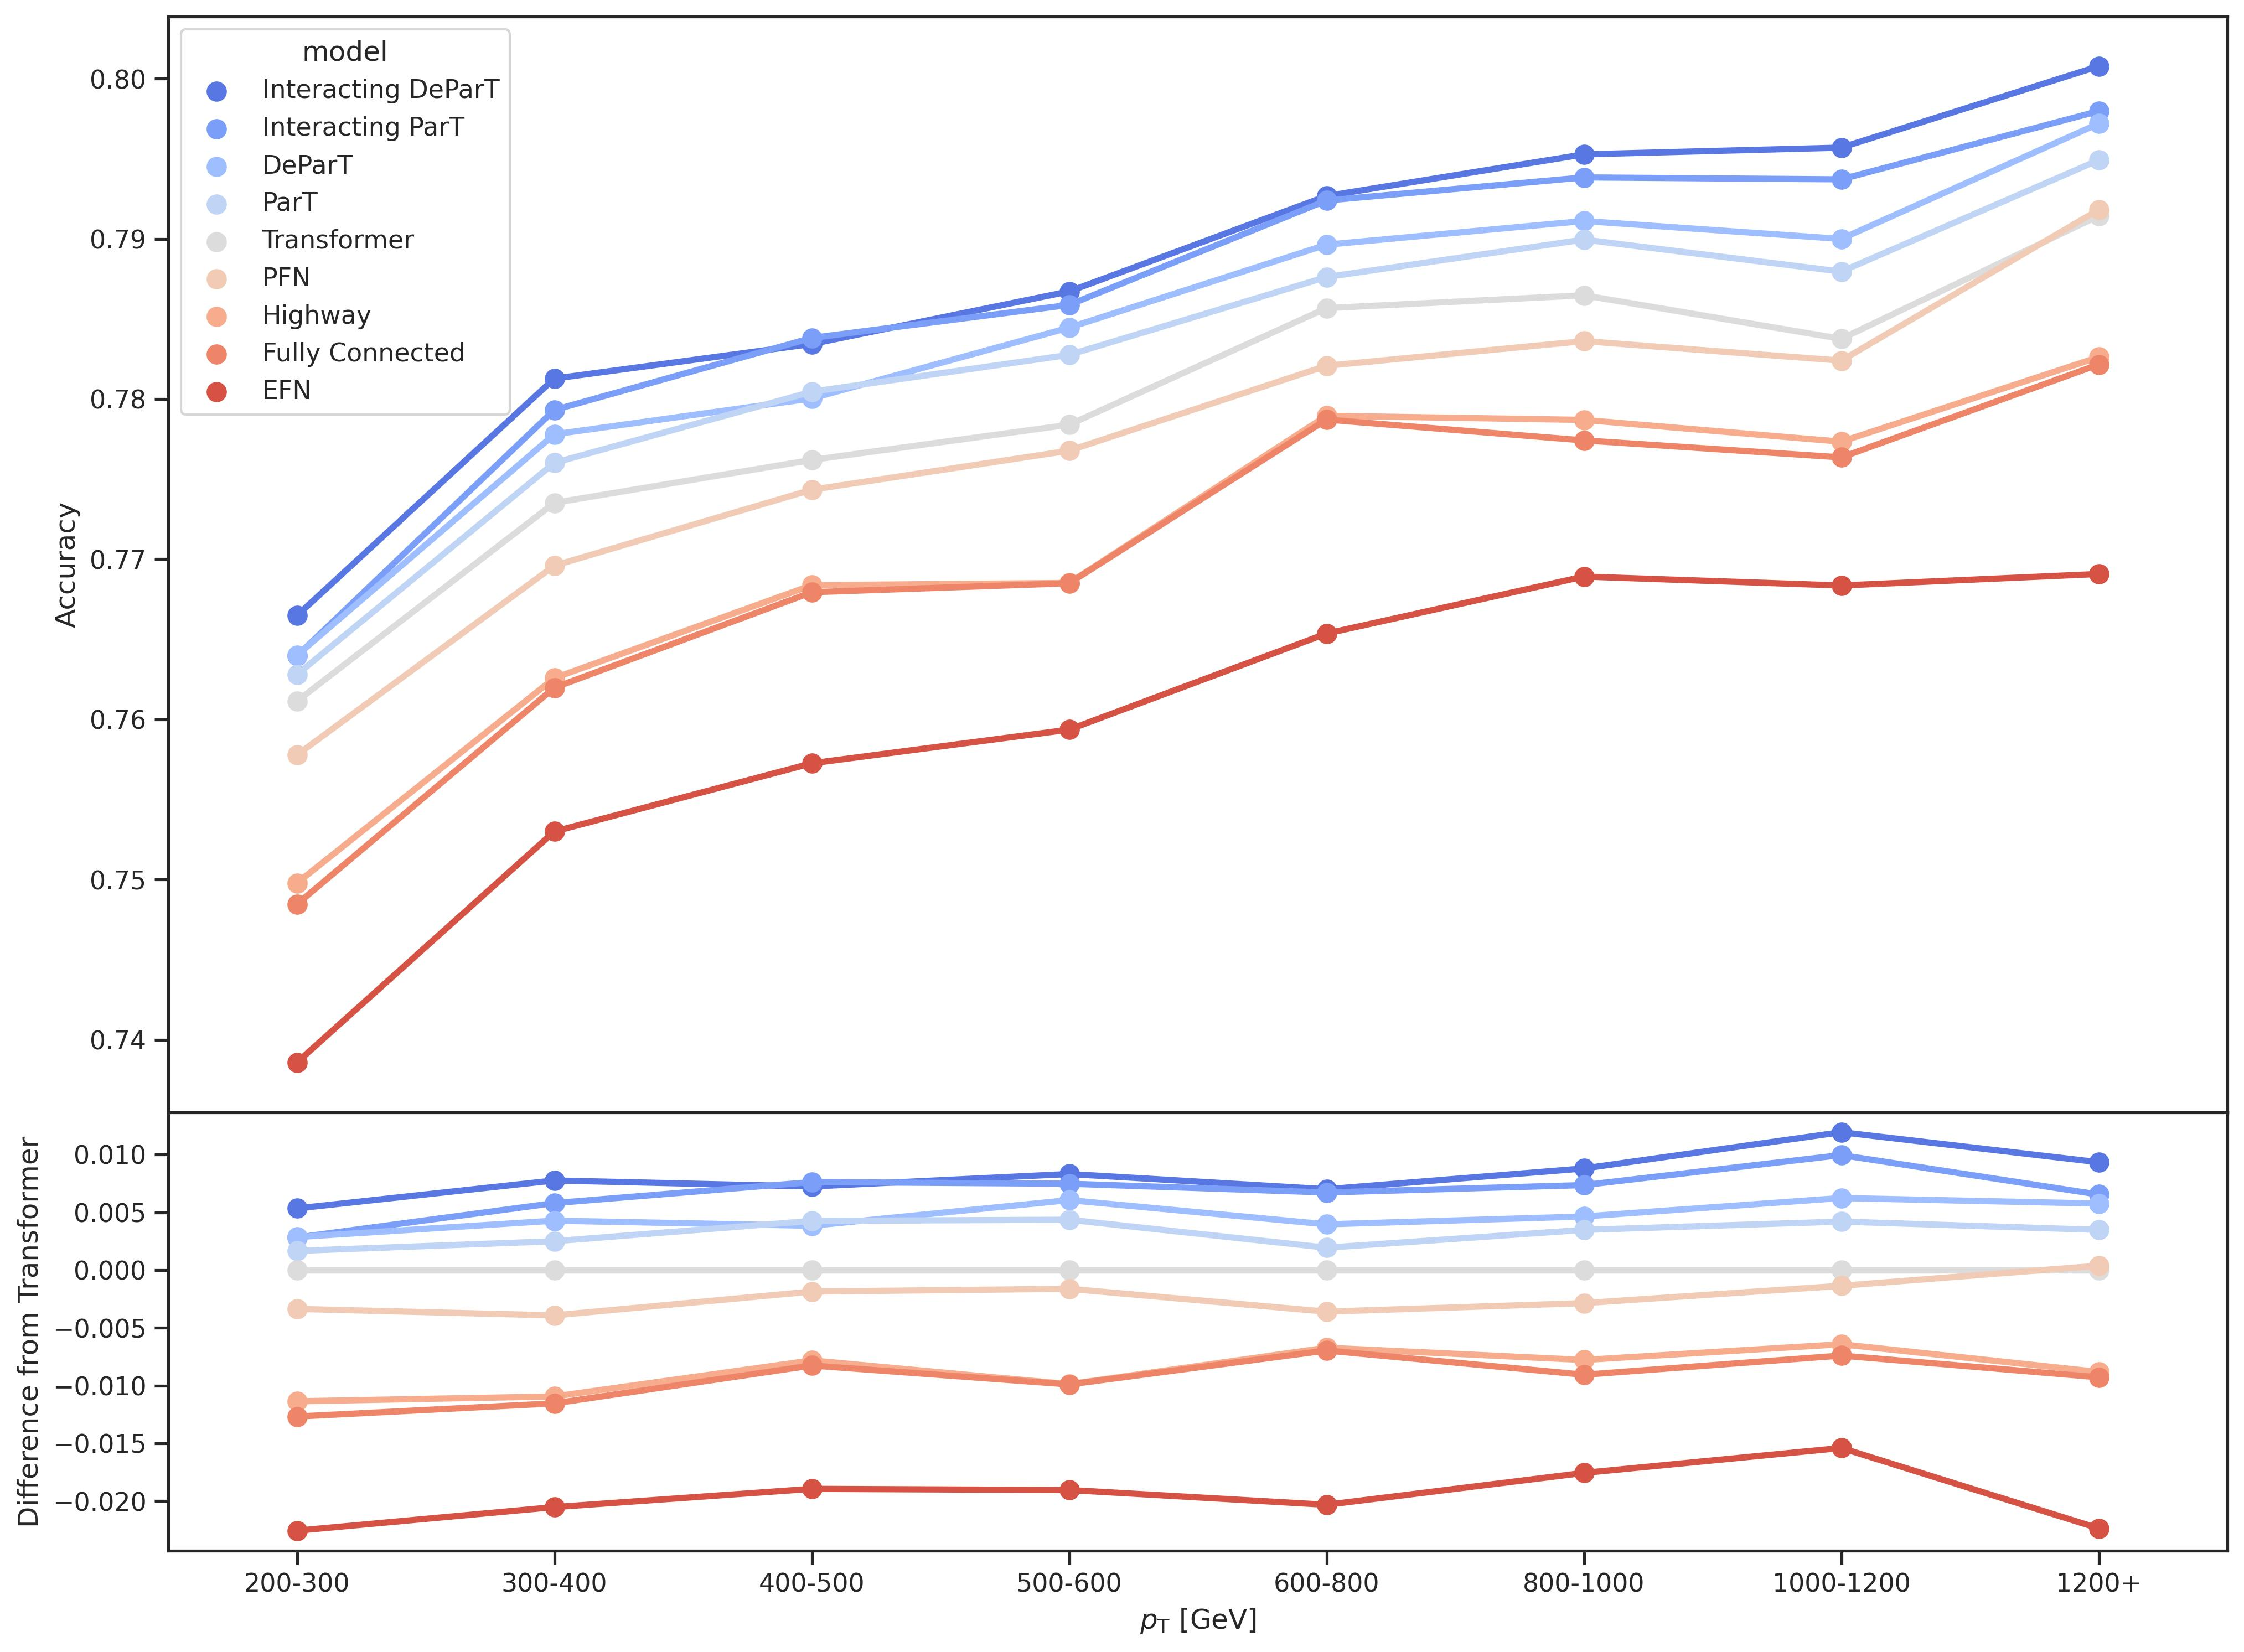
\includegraphics[width=1\linewidth]{src/plots/results/pT_dep/relative_accuracy_zoom.jpg}
    \caption{Zoom to the accuracy of the models as a function of $\pT$ and relative to the Transformer model.}
    \label{fig:pt_dep_acc_zoom}
\end{figure}
\begin{figure}[htb]
    \centering
    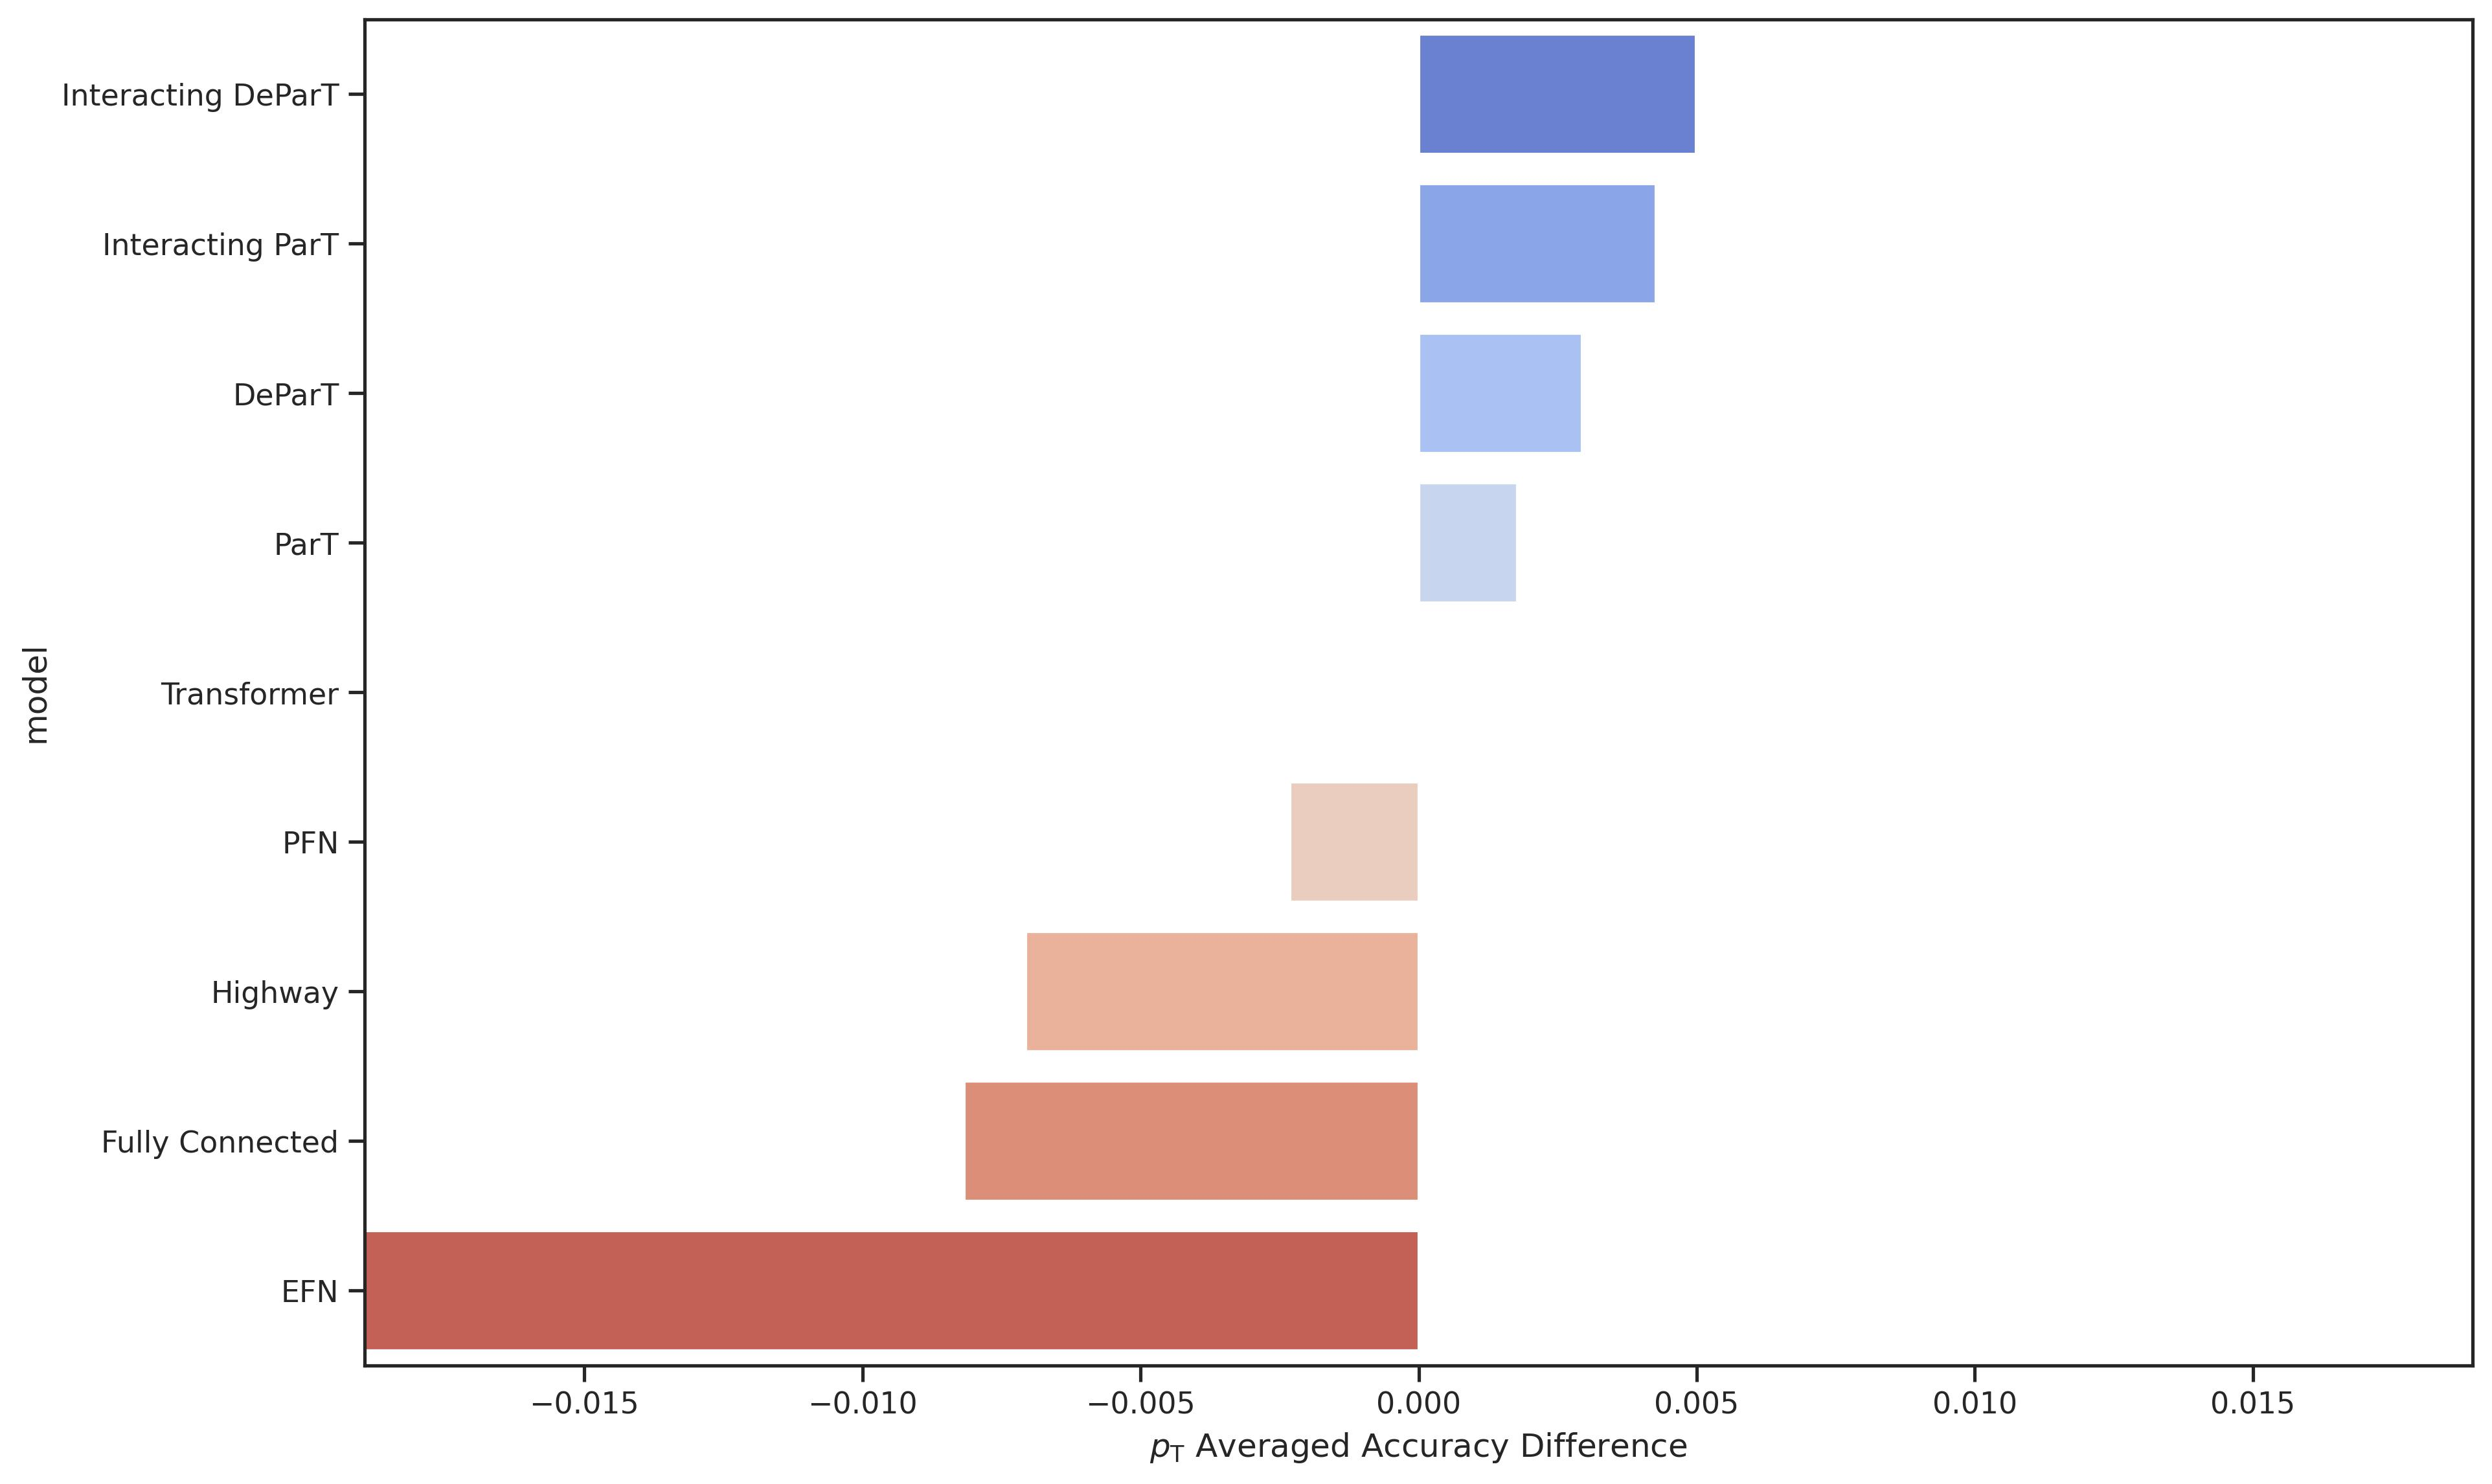
\includegraphics[width=1\linewidth]{src/plots/results/pT_dep/relative_error.jpg}
    \caption{$\pT$ averaged difference from the Transformer model.}
    \label{fig:pt_dep_diff}
\end{figure}
In \cref{fig:pt_dep_acc}, we can see that the accuracy of the models is dependent on the $\pT$ of the jets.
The higher the $\pT$, the better the performance.
At low $\pT$, there seems to be an upper bound on the accuracy since none of the models can improve as much as they do at higher $\pT$.
Different factors may cause this.
The pure definition of \texttt{PartonTruthLabelID} can be inconsistent at low $\pT$, or the jet clustering algorithm has problems such as distinguishing hard jets and pileup.
Also, at higher $\pT$, above 200 GeV, the performance is more or less stable with $\pT$.

The model's ordering is more visible if we zoom in on the high $\pT$ range, as seen in \cref{fig:pt_dep_acc_zoom}.
The \EFN is the worst-performing model, which indicates that some kind of mapping of energy variables (like $\pT$ or $E$) is necessary for the model to perform well and instead tackle the IRC safety differently.
The \highway is almost identical to the \fc, which is unsurprising, as they are very similar models.
The main advantage is that the \highway diverges less than the \fc, but using the LAMB optimizer makes the \fc converge to the same result. \footnote{When we trained them with Adam optimizer, the \highway performed better.}

The averaged difference from \trans is displayed in \cref{fig:pt_dep_diff} to emphasize the relative model performances. 

Additional metrics are plotted in \cref{sec:app_pt_dep}.

\FloatBarrier

\subsection{Pseudo-rapidity Dependence}
\label{sec:eta_dependance}
\begin{figure}[htb]
    \centering
    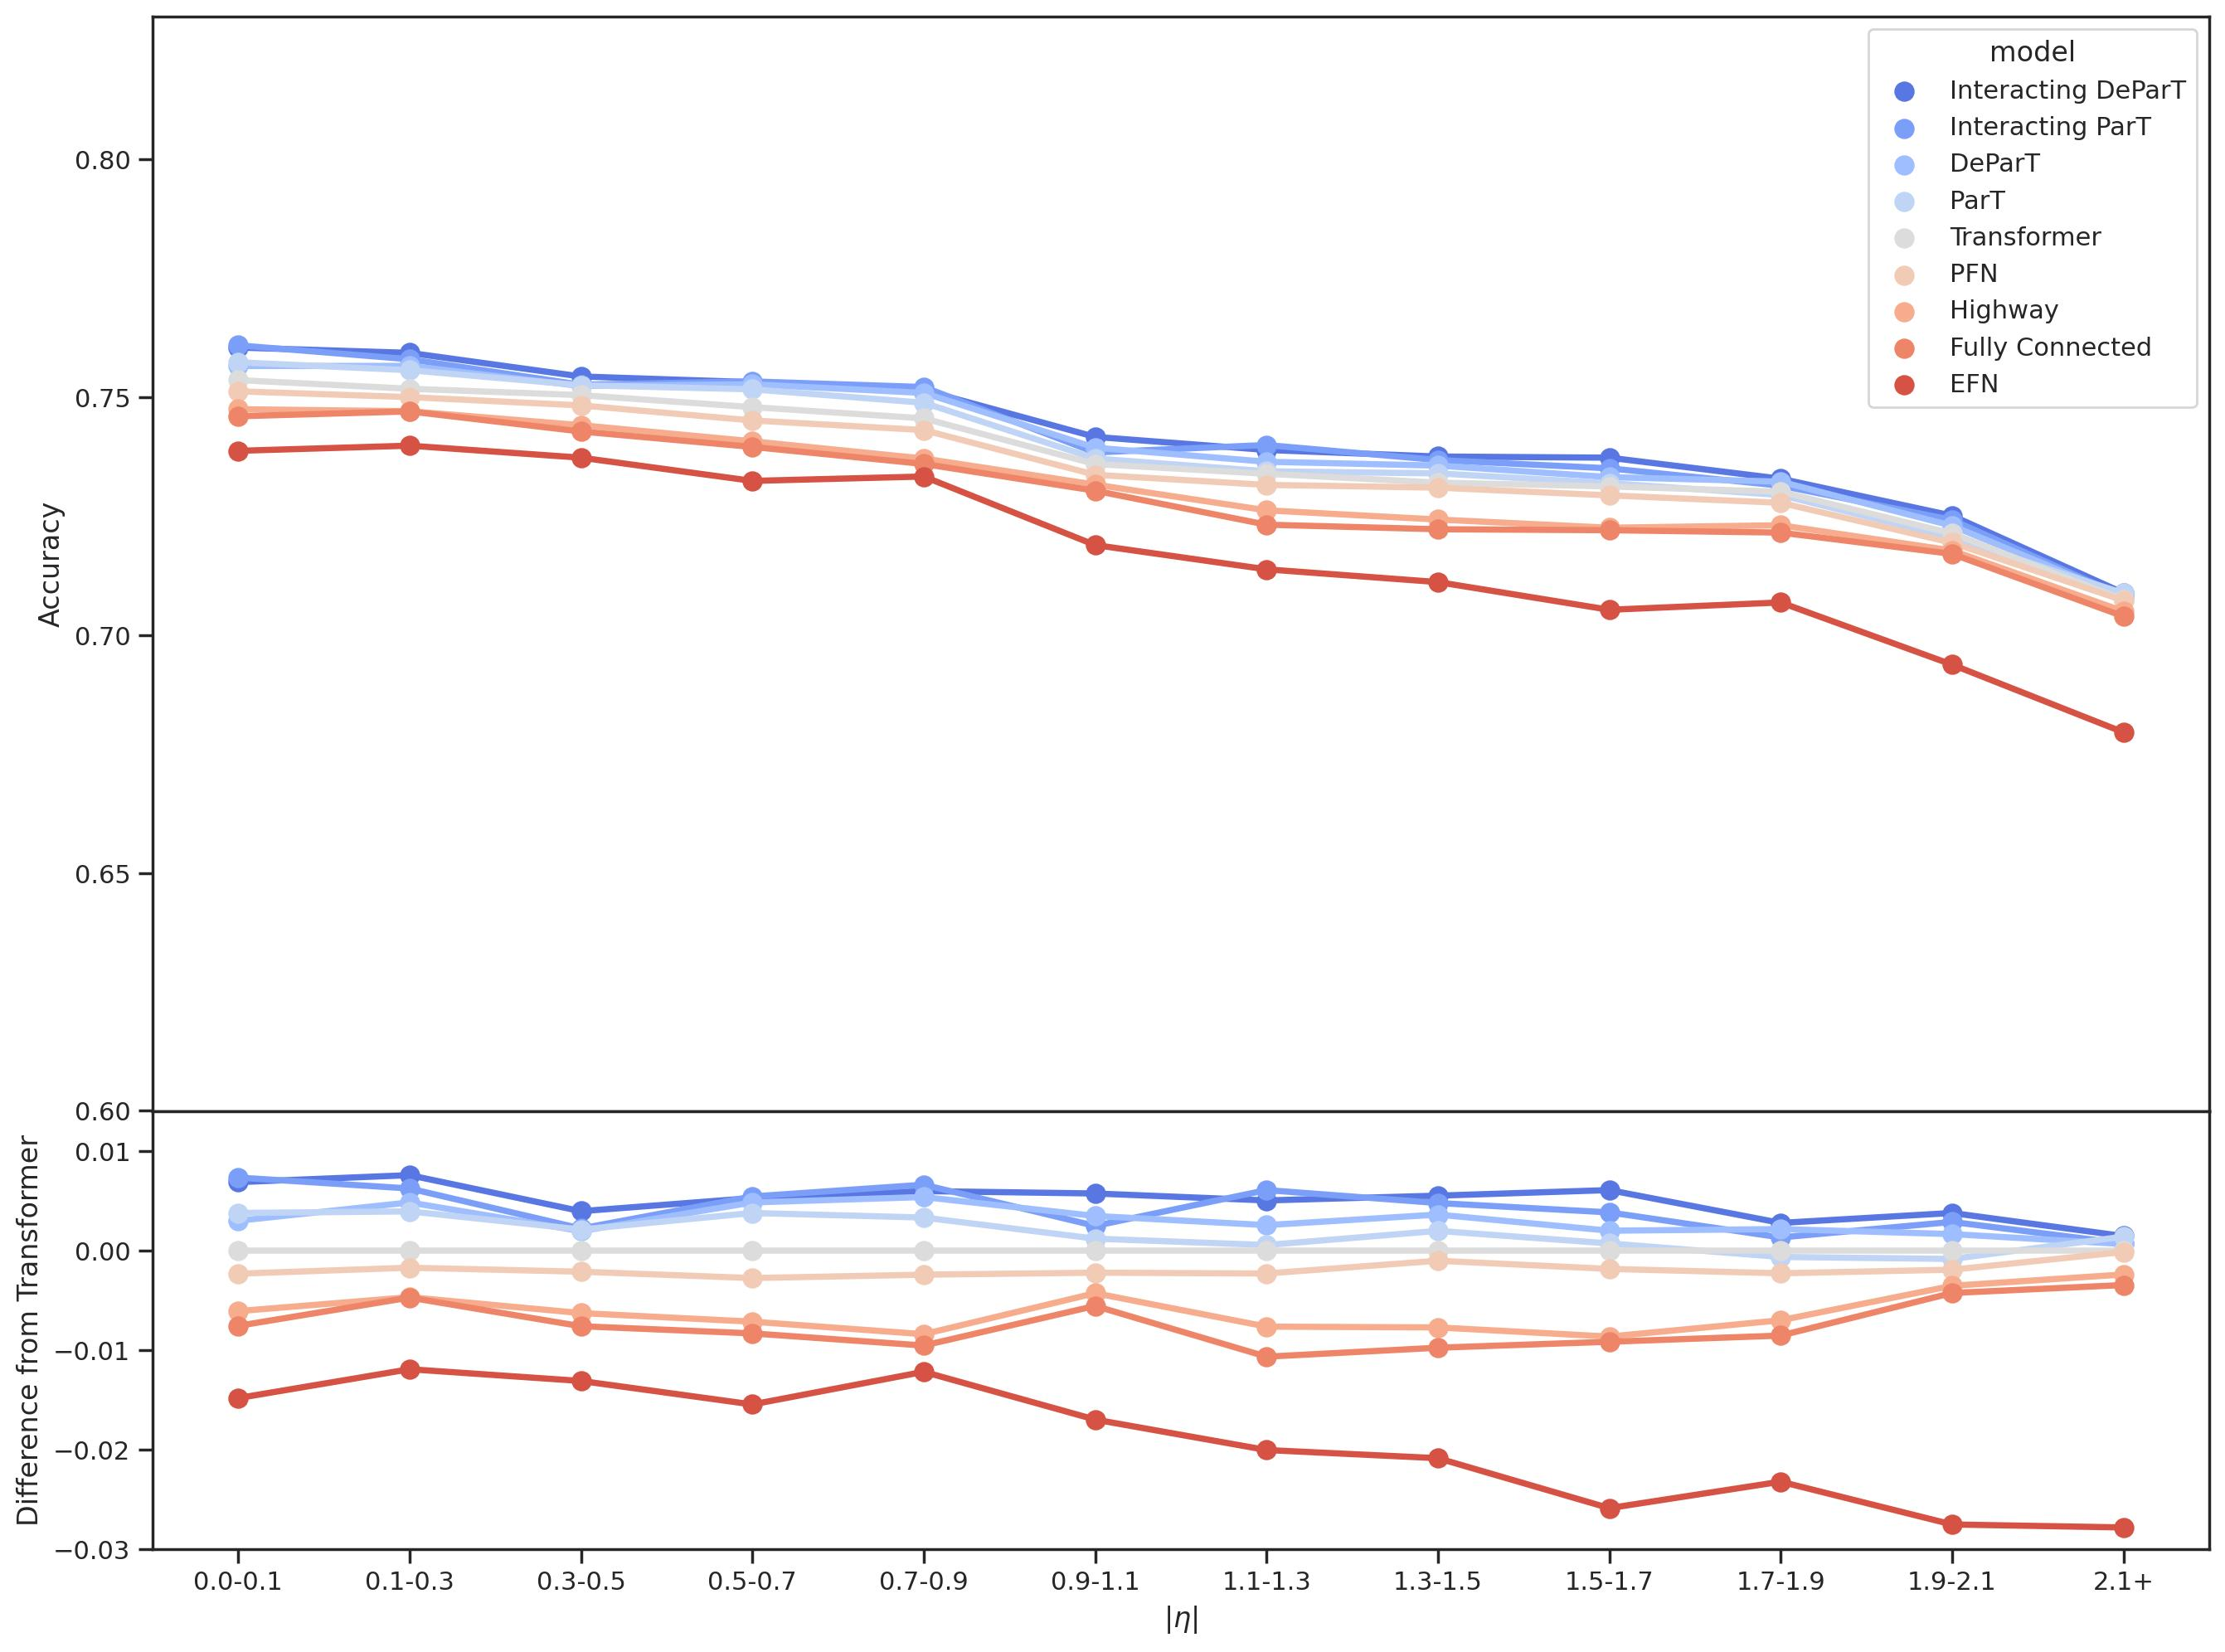
\includegraphics[width=1\linewidth]{src/plots/results/eta_dep/relative_accuracy.jpg}
    \caption{Accuracy of the models as a function of $|\eta|$ and relative to the Transformer model.}
    \label{fig:eta_dep_acc}
\end{figure}
\begin{figure}[htb]
    \centering
    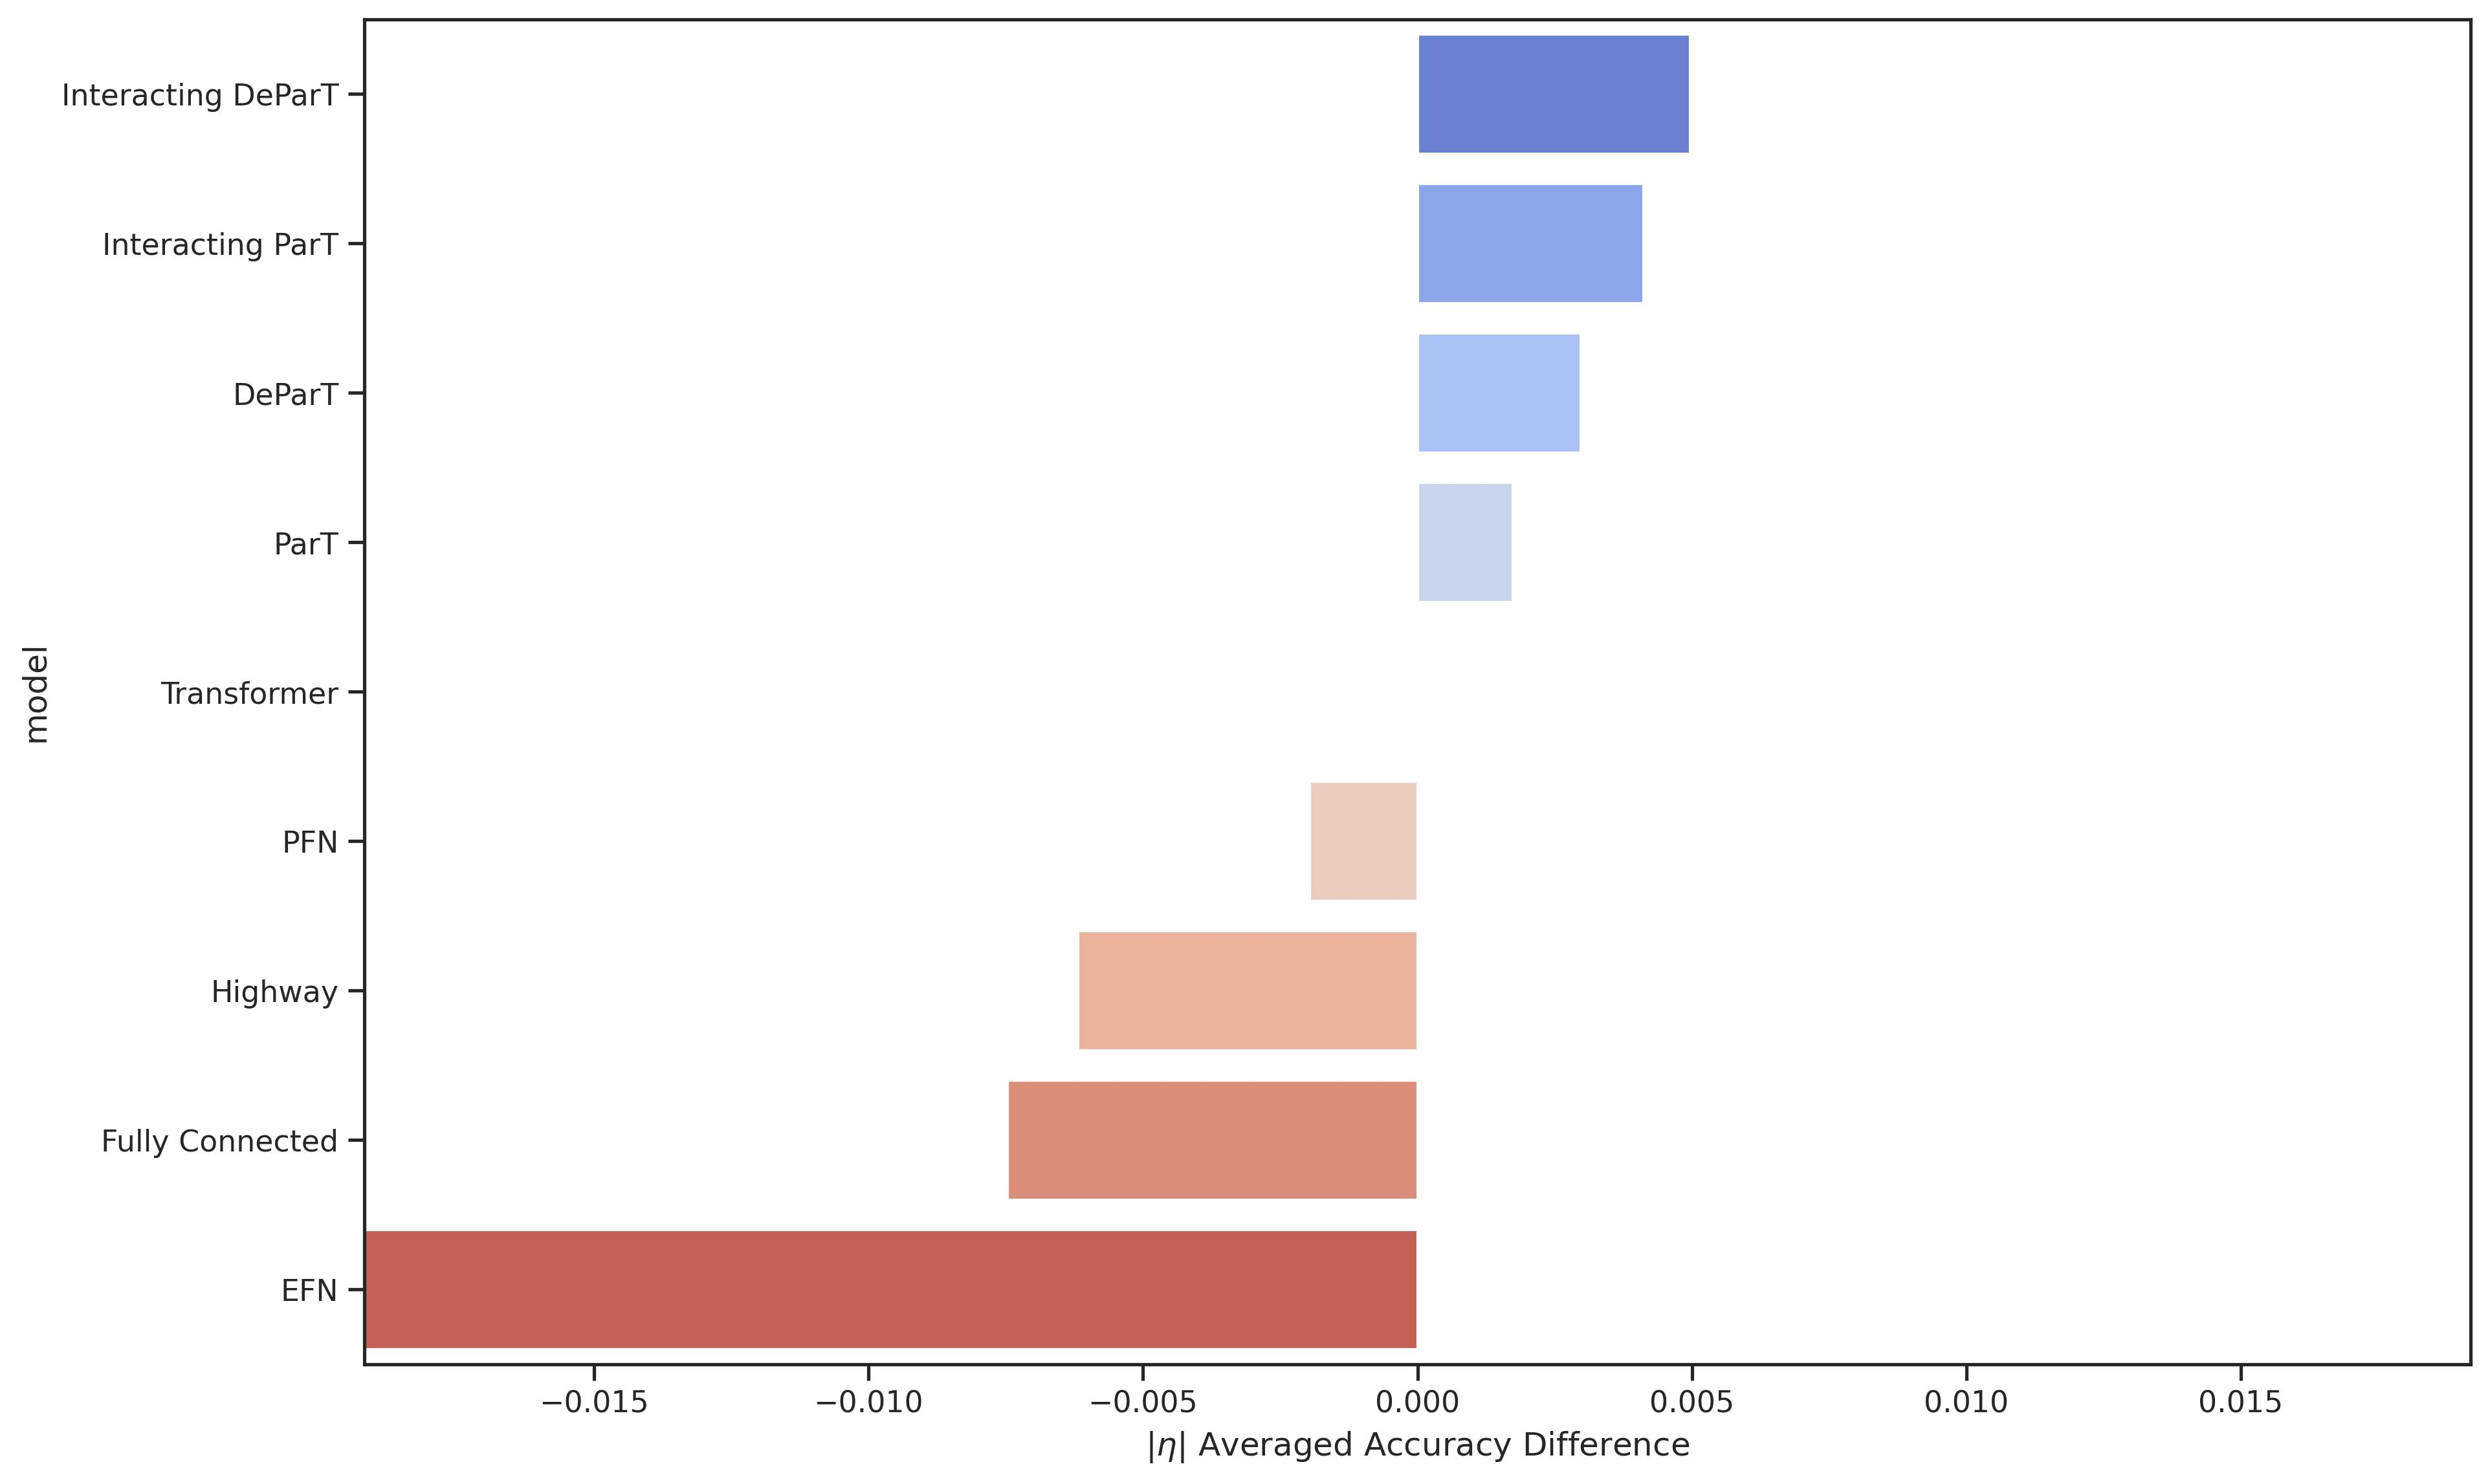
\includegraphics[width=1\linewidth]{src/plots/results/eta_dep/relative_error.jpg}
    \caption{$|\eta|$ averaged difference from the Transformer model.}
    \label{fig:eta_dep_diff}
\end{figure}
In \cref{fig:eta_dep_acc}, we can see that the accuracy of the models is way less dependent on the $|\eta|$ than on the $\pT$.
The only slightly different part is at $|\eta| \approx 2.1$, where the tracker cannot measure the full jets.
We also see that \EFN is more dependent on the $|\eta|$ than the other models.
This may be caused by the fact that \EFN uses per \PFO mapping only on the angular variables causing the model to be more sensitive to the $|\eta|$.

The relative performance of the models, shown in \cref{fig:eta_dep_diff}, is similar to the $\pT$ dependence.

Additional metrics are plotted in \cref{sec:app_eta_dep}.

\FloatBarrier

\subsection{Pileup Dependence}
\label{sec:mu_dependance}
\begin{figure}[htb]
    \centering
    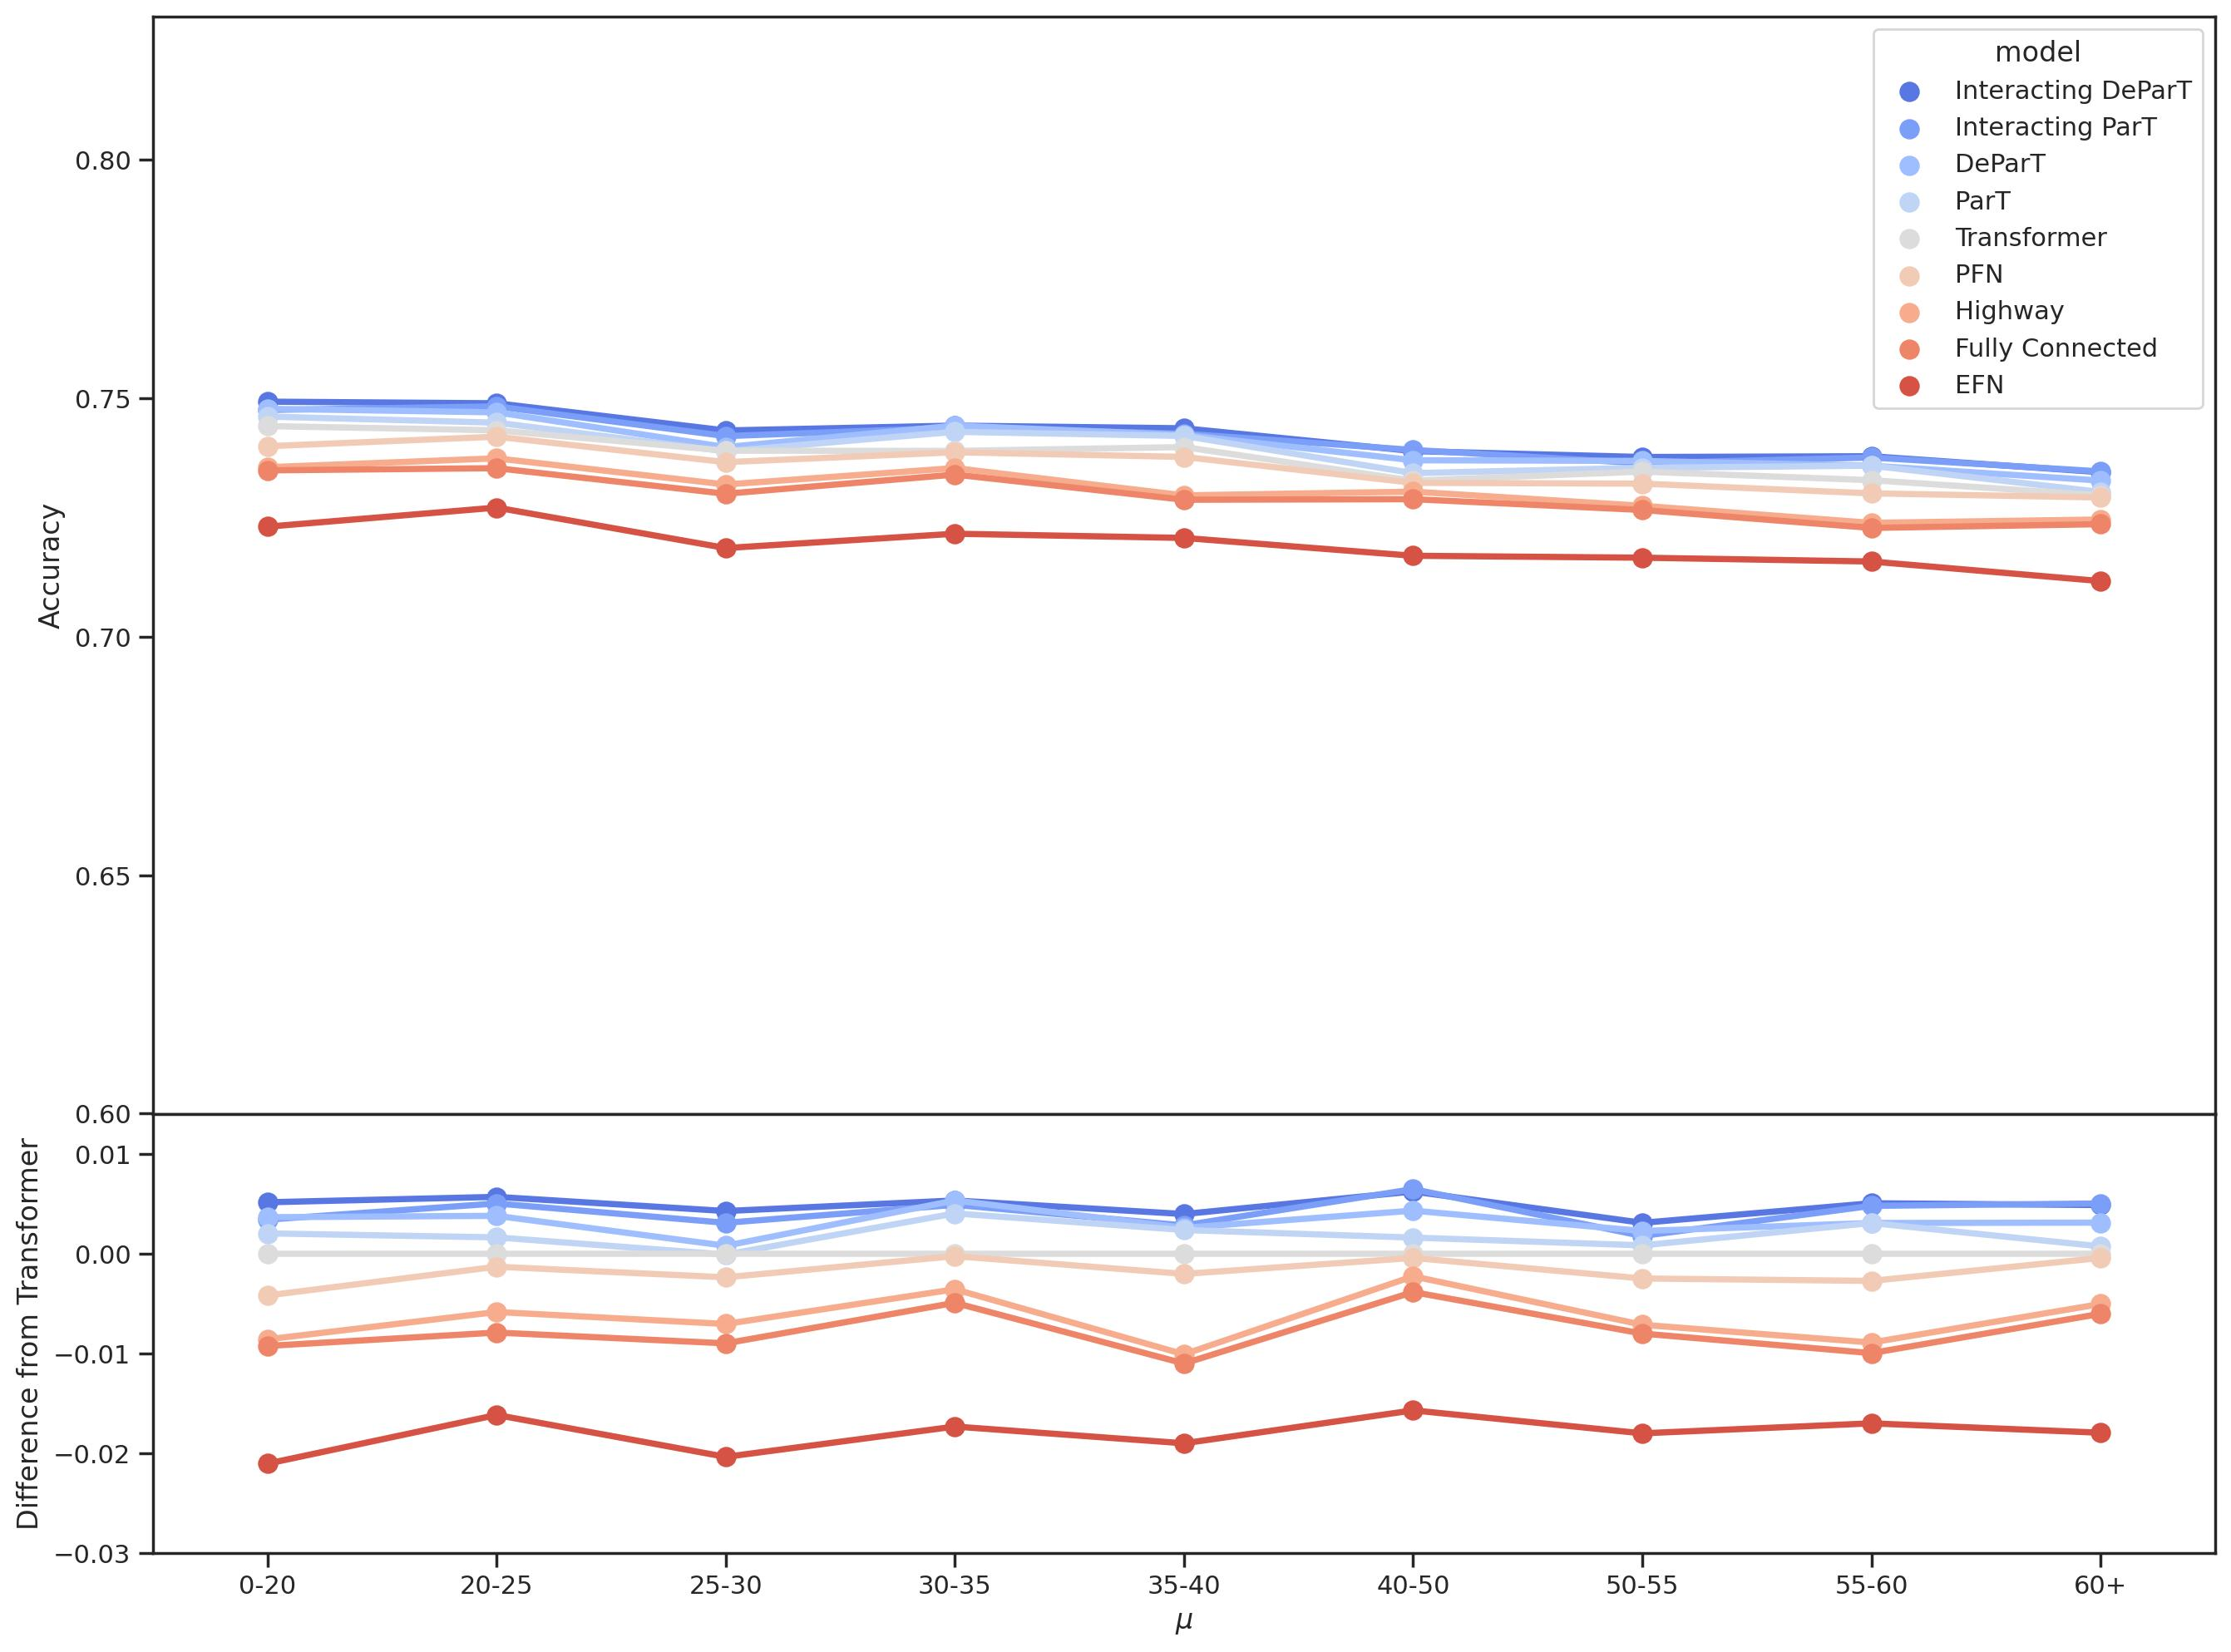
\includegraphics[width=1\linewidth]{src/plots/results/mu_dep/relative_accuracy.jpg}
    \caption{Accuracy of the models as a function of $\mu$ and relative to the Transformer model.}
    \label{fig:mu_dep_acc}
\end{figure}
\begin{figure}[htb]
    \centering
    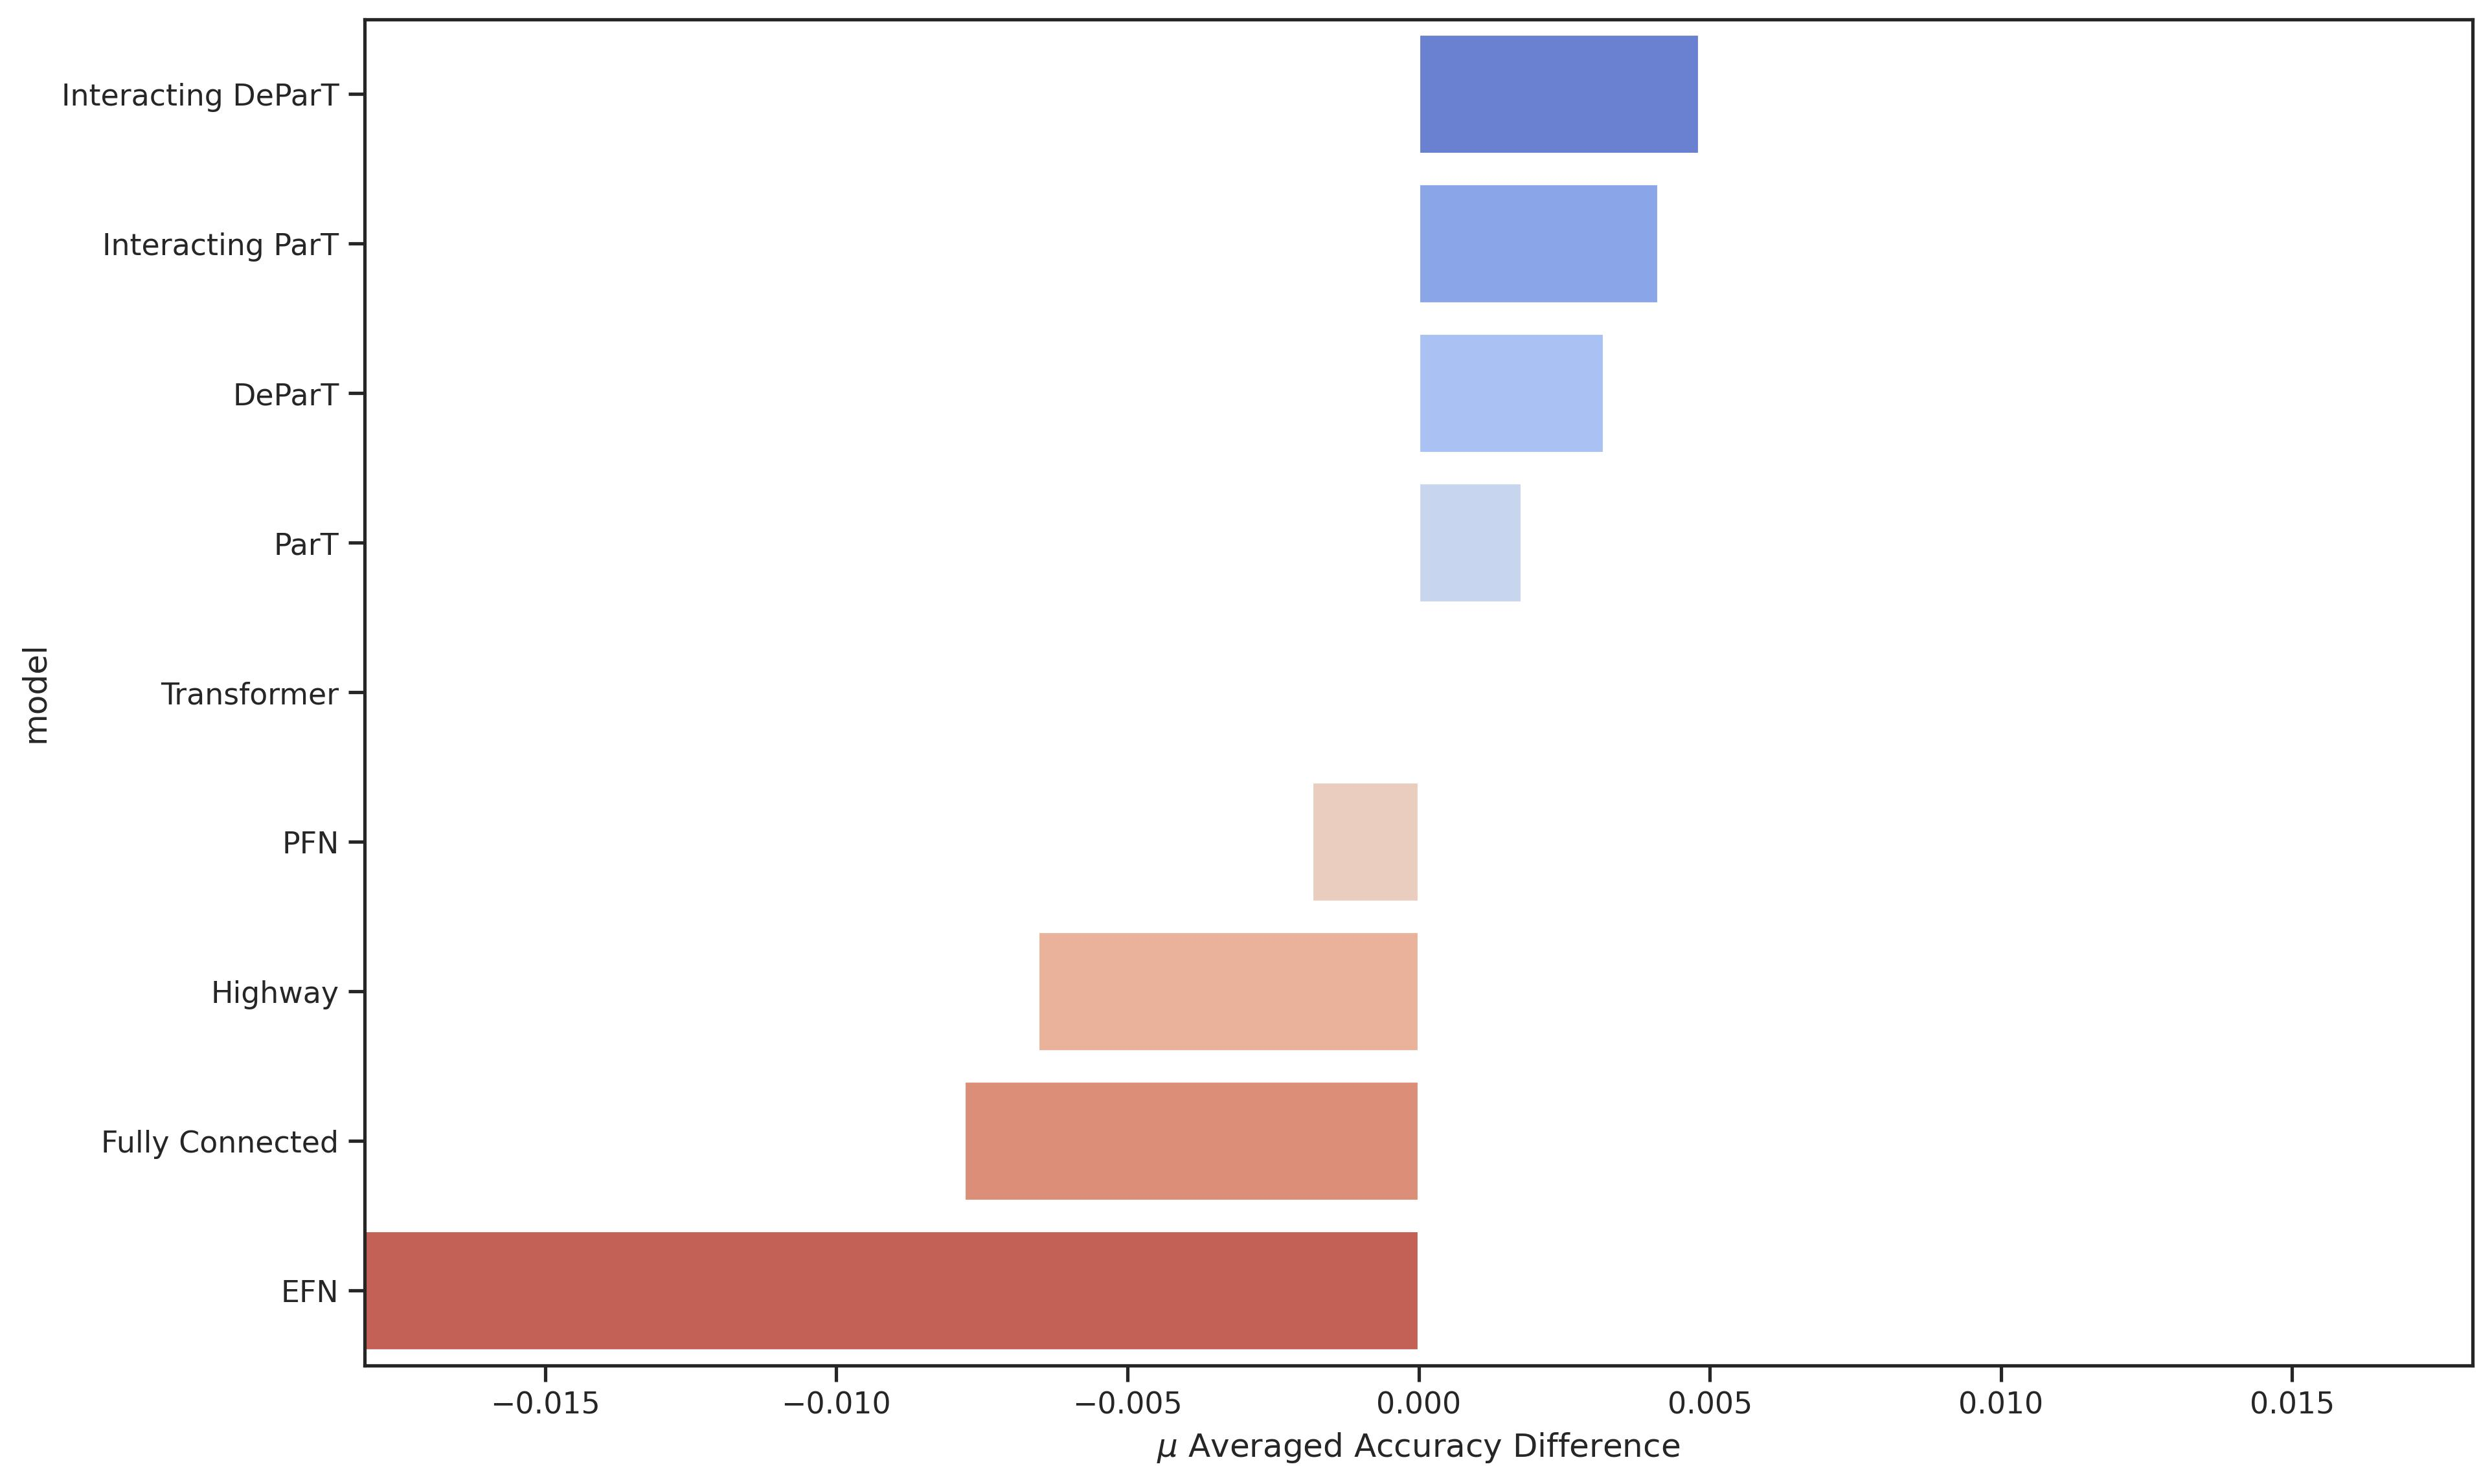
\includegraphics[width=1\linewidth]{src/plots/results/mu_dep/relative_error.jpg}
    \caption{$\mu$ averaged difference from the Transformer model.}
    \label{fig:mu_dep_diff}
\end{figure}
Dependence on the pileup $\mu$ is shown in \cref{fig:mu_dep_acc}.
It impacts the performance of the models the least out of the three variables.
The trend is slightly downward, but it is not significant.

The relative performance of the models, shown in \cref{fig:mu_dep_diff}, is similar to the $\pT$ and $|\eta|$ dependence.

Additional metrics are plotted in \cref{sec:app_pileup_dep}.